\documentclass[../thesis.tex]{subfiles}
\begin{document}

\chapter{Parametric Study}
\label{chp: para_stud}
The parametric study is done to distinguish between the influence of the thermophysical properties against the one coming from convection on the front's shape and metrics. To achieve that different inlet velocities are used to investigate the influence of convection. To get the influence of the thermophysical properties different diffusion coefficients and viscosities are set. This results in the combination of parameters studied as shown in \autoref{tab: cases}.

Within the parametric study three different reactor geometries are simulated. The different conditions set for each case lead to different front shapes. Two of these front shapes for two example cases can be seen in \autoref{fig: shape_examp}.
\begin{figure}[htb]
	\centering
	\subfloat[\centering front shape for  h = 0.6mm Pe = 2050 Sc = 12000]{{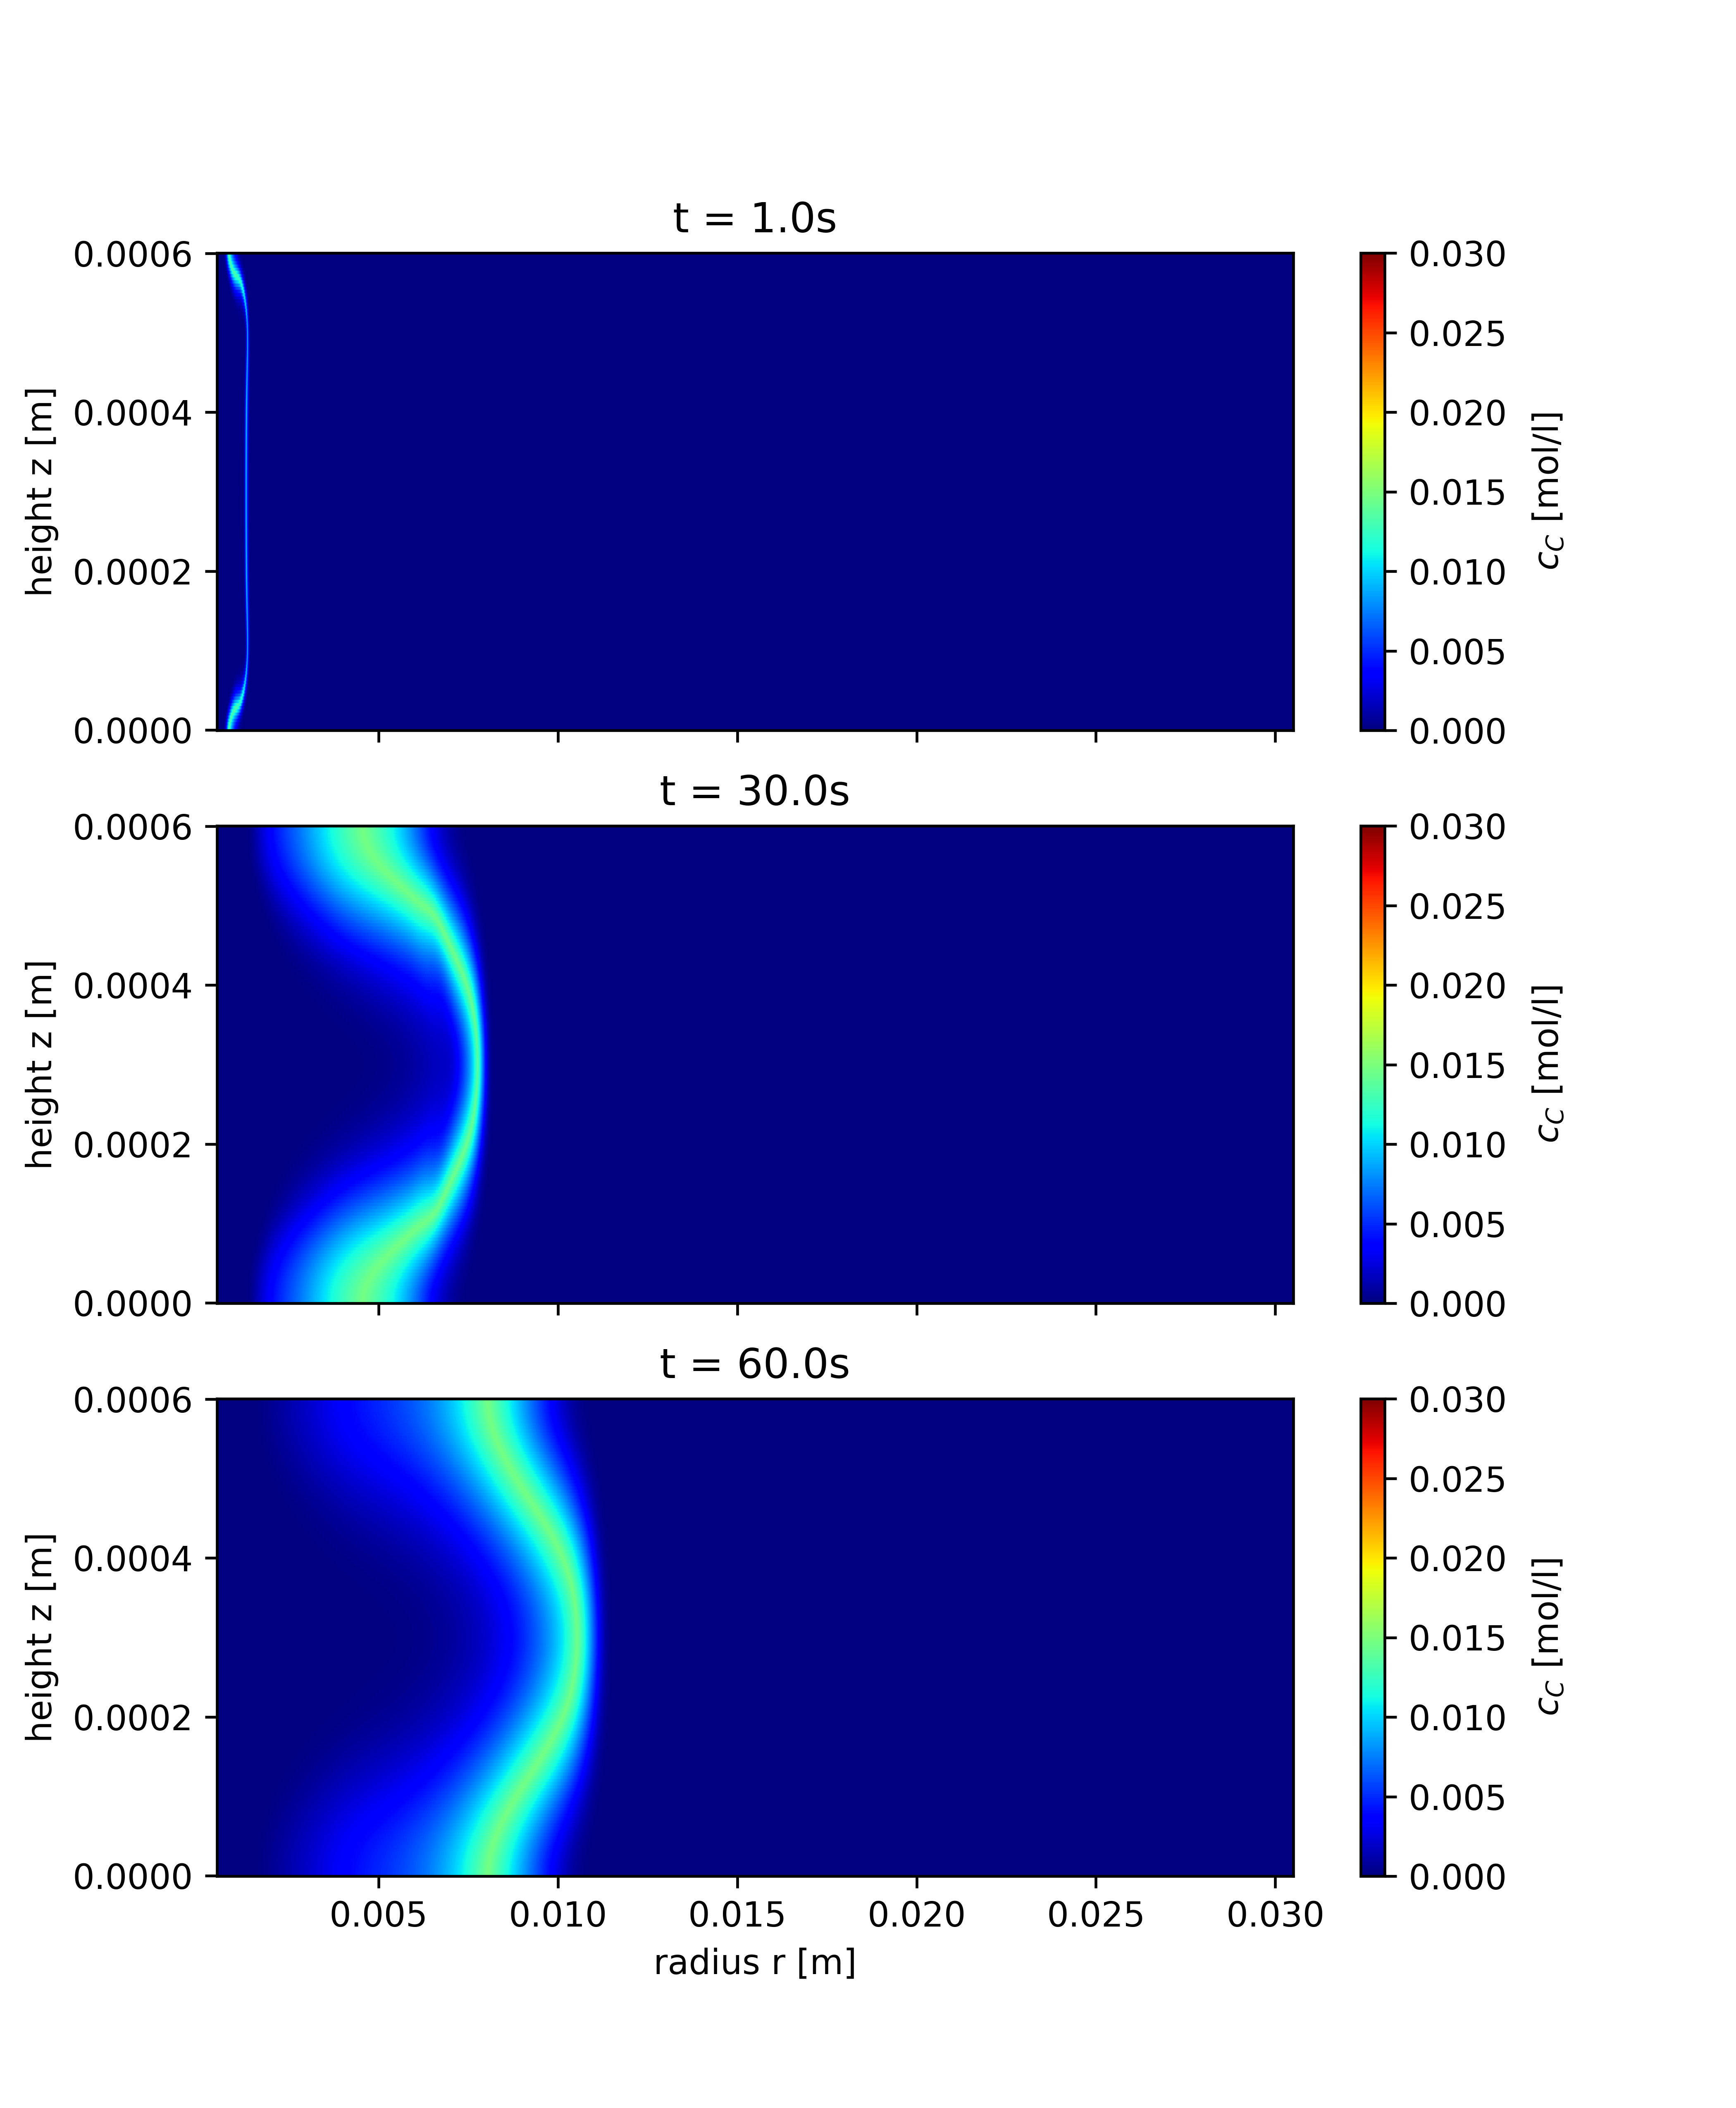
\includegraphics[angle=0, scale=0.41]{front_shape1} }}%
	\qquad
	\subfloat[\centering front shape for  h = 0.2mm Pe = 2050 Sc = 2430]{{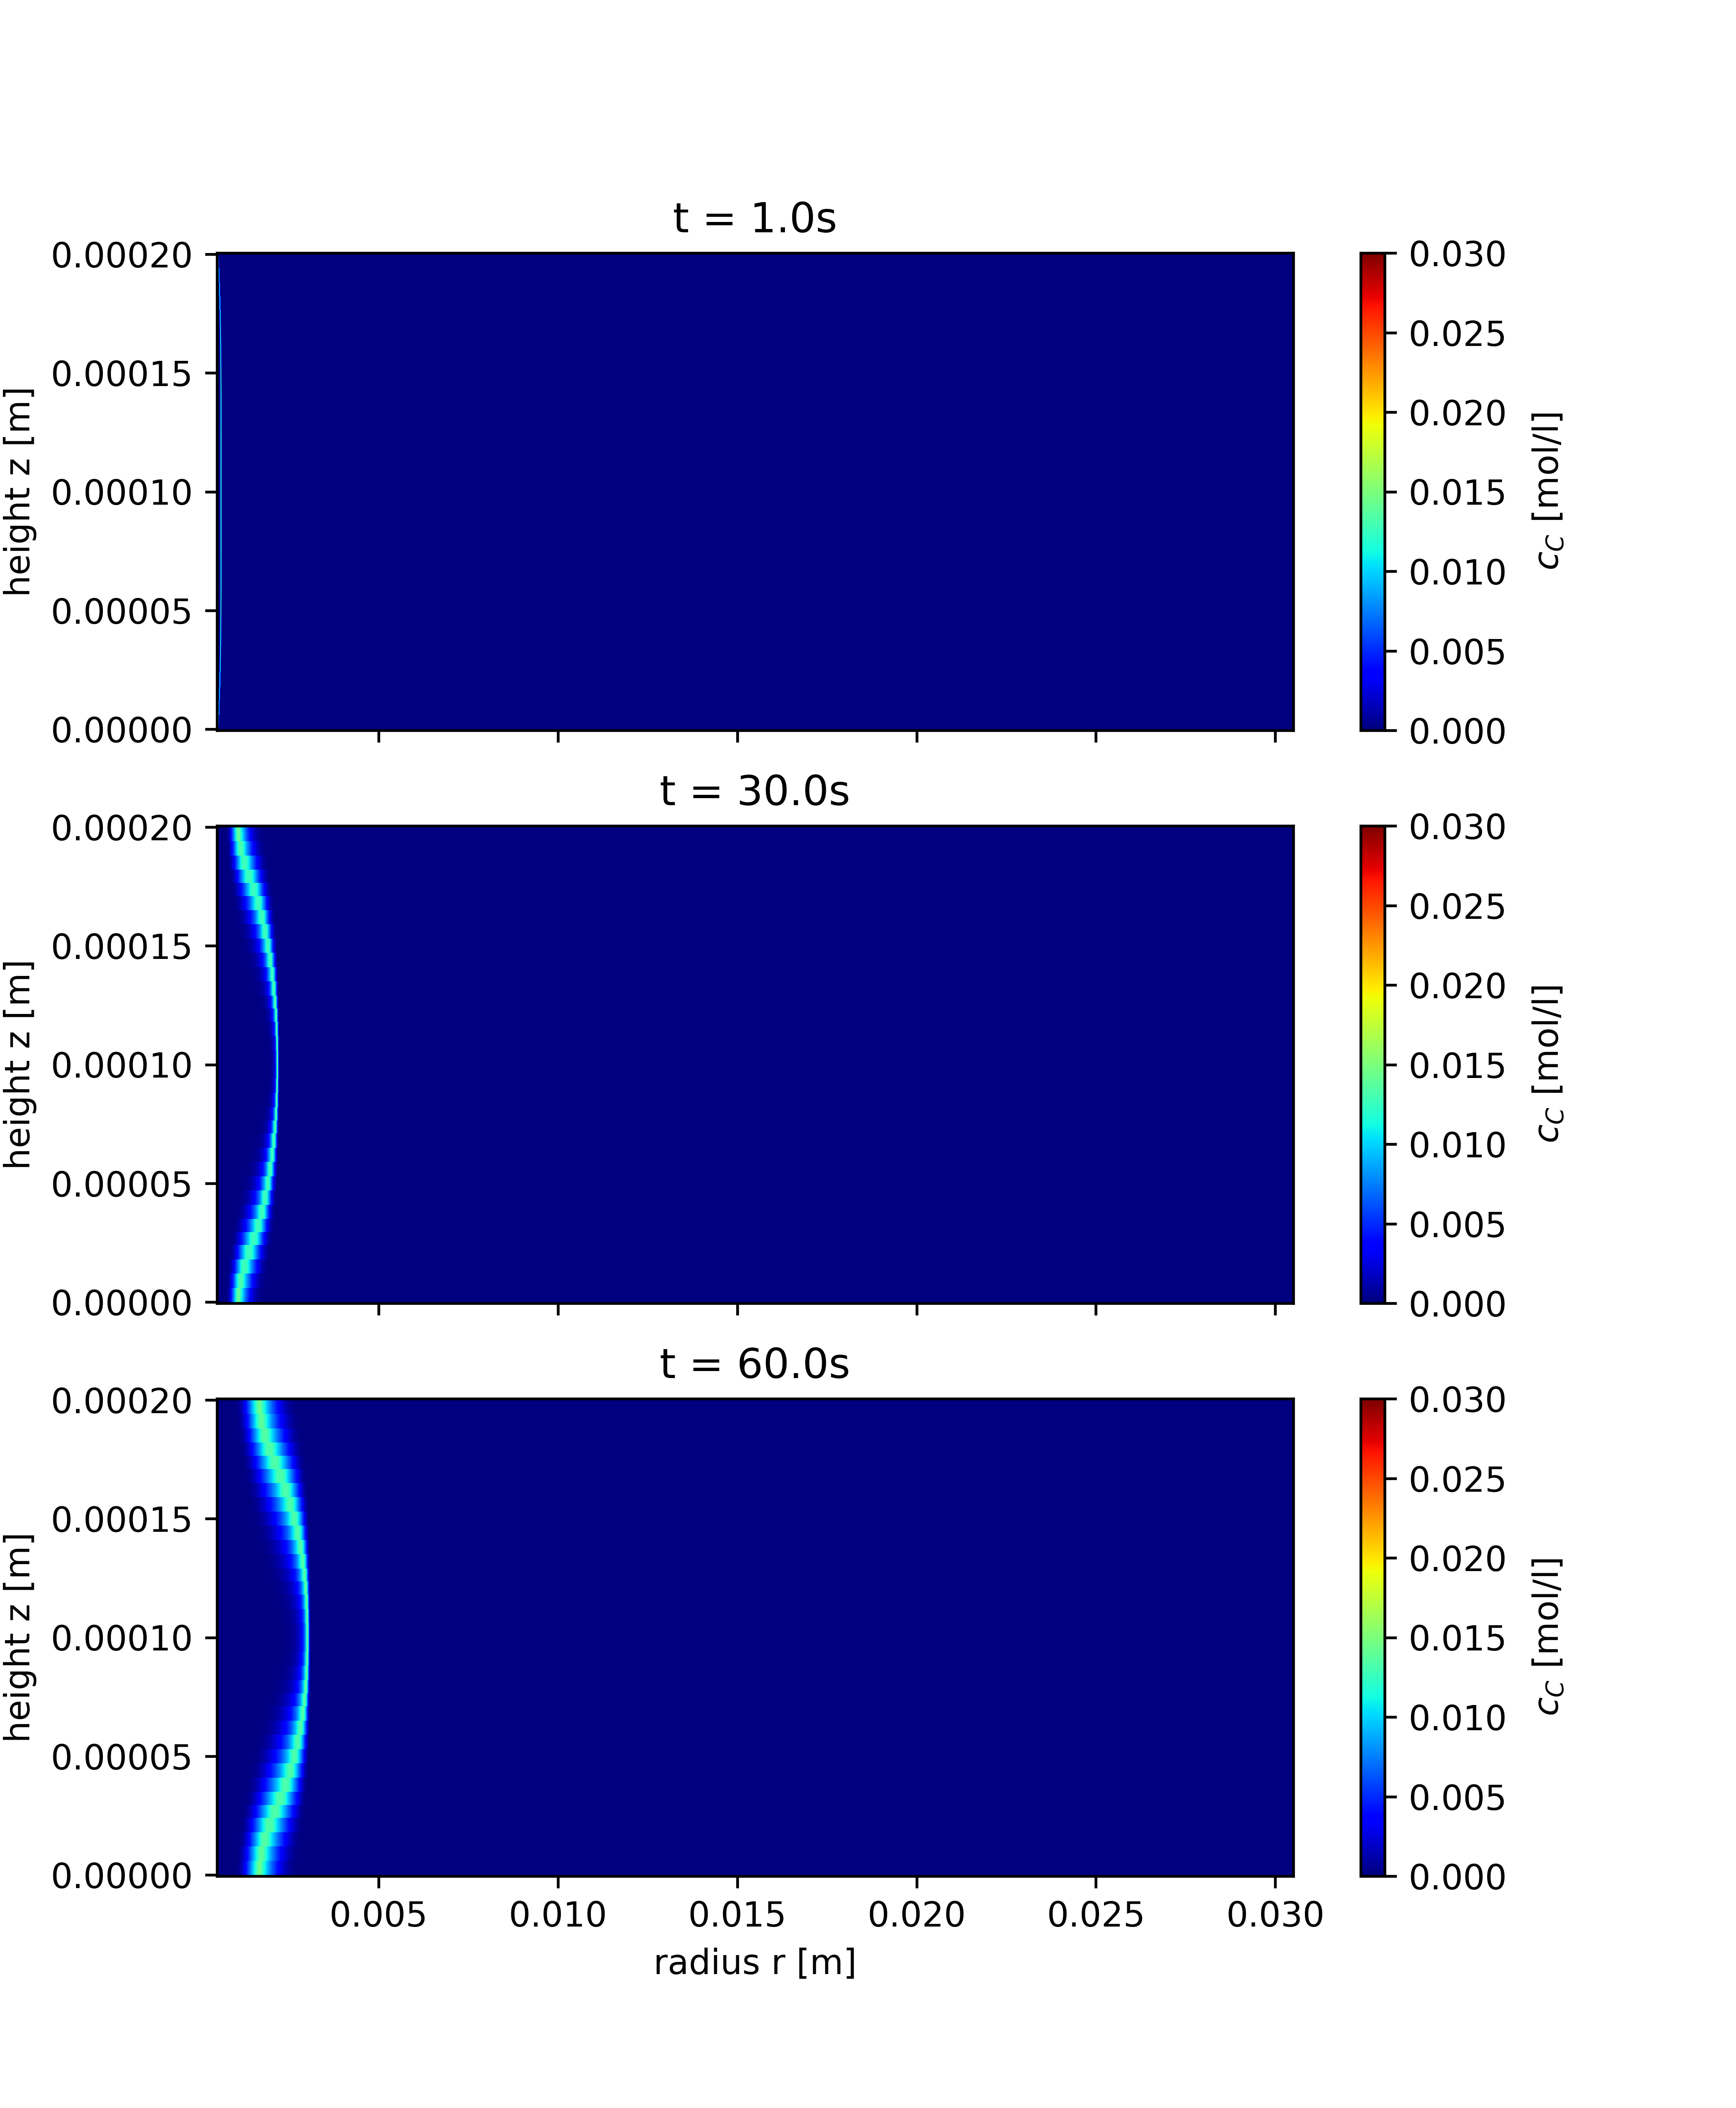
\includegraphics[angle=0, scale=0.41]{front_shape2} }}%
	\caption{Two example front shapes as a result of different flow conditions}%
	\label{fig: shape_examp}%
\end{figure}
Comparing the cases shown in \autoref{fig: shape_examp} it becomes clear, that the reactor gap height and thermophysical properties show a significant influence on the fronts progression and curvature. In addition to that the front's width is also influenced. A more detailed analysis of the front's position, width and the total amount of product formed is given in the following sections. 

\section{Front Positions}

The front positions behave in a similar way for all 3 reactor geometries. In \autoref{fig: front_pos_h2_Sc12000} and \autoref{fig: front_pos_h2_Sc2430} the positions for both Schmidt numbers are shown for the geometry containing a gap height of 0.2mm.
\begin{figure}[htbp]
	\centering
	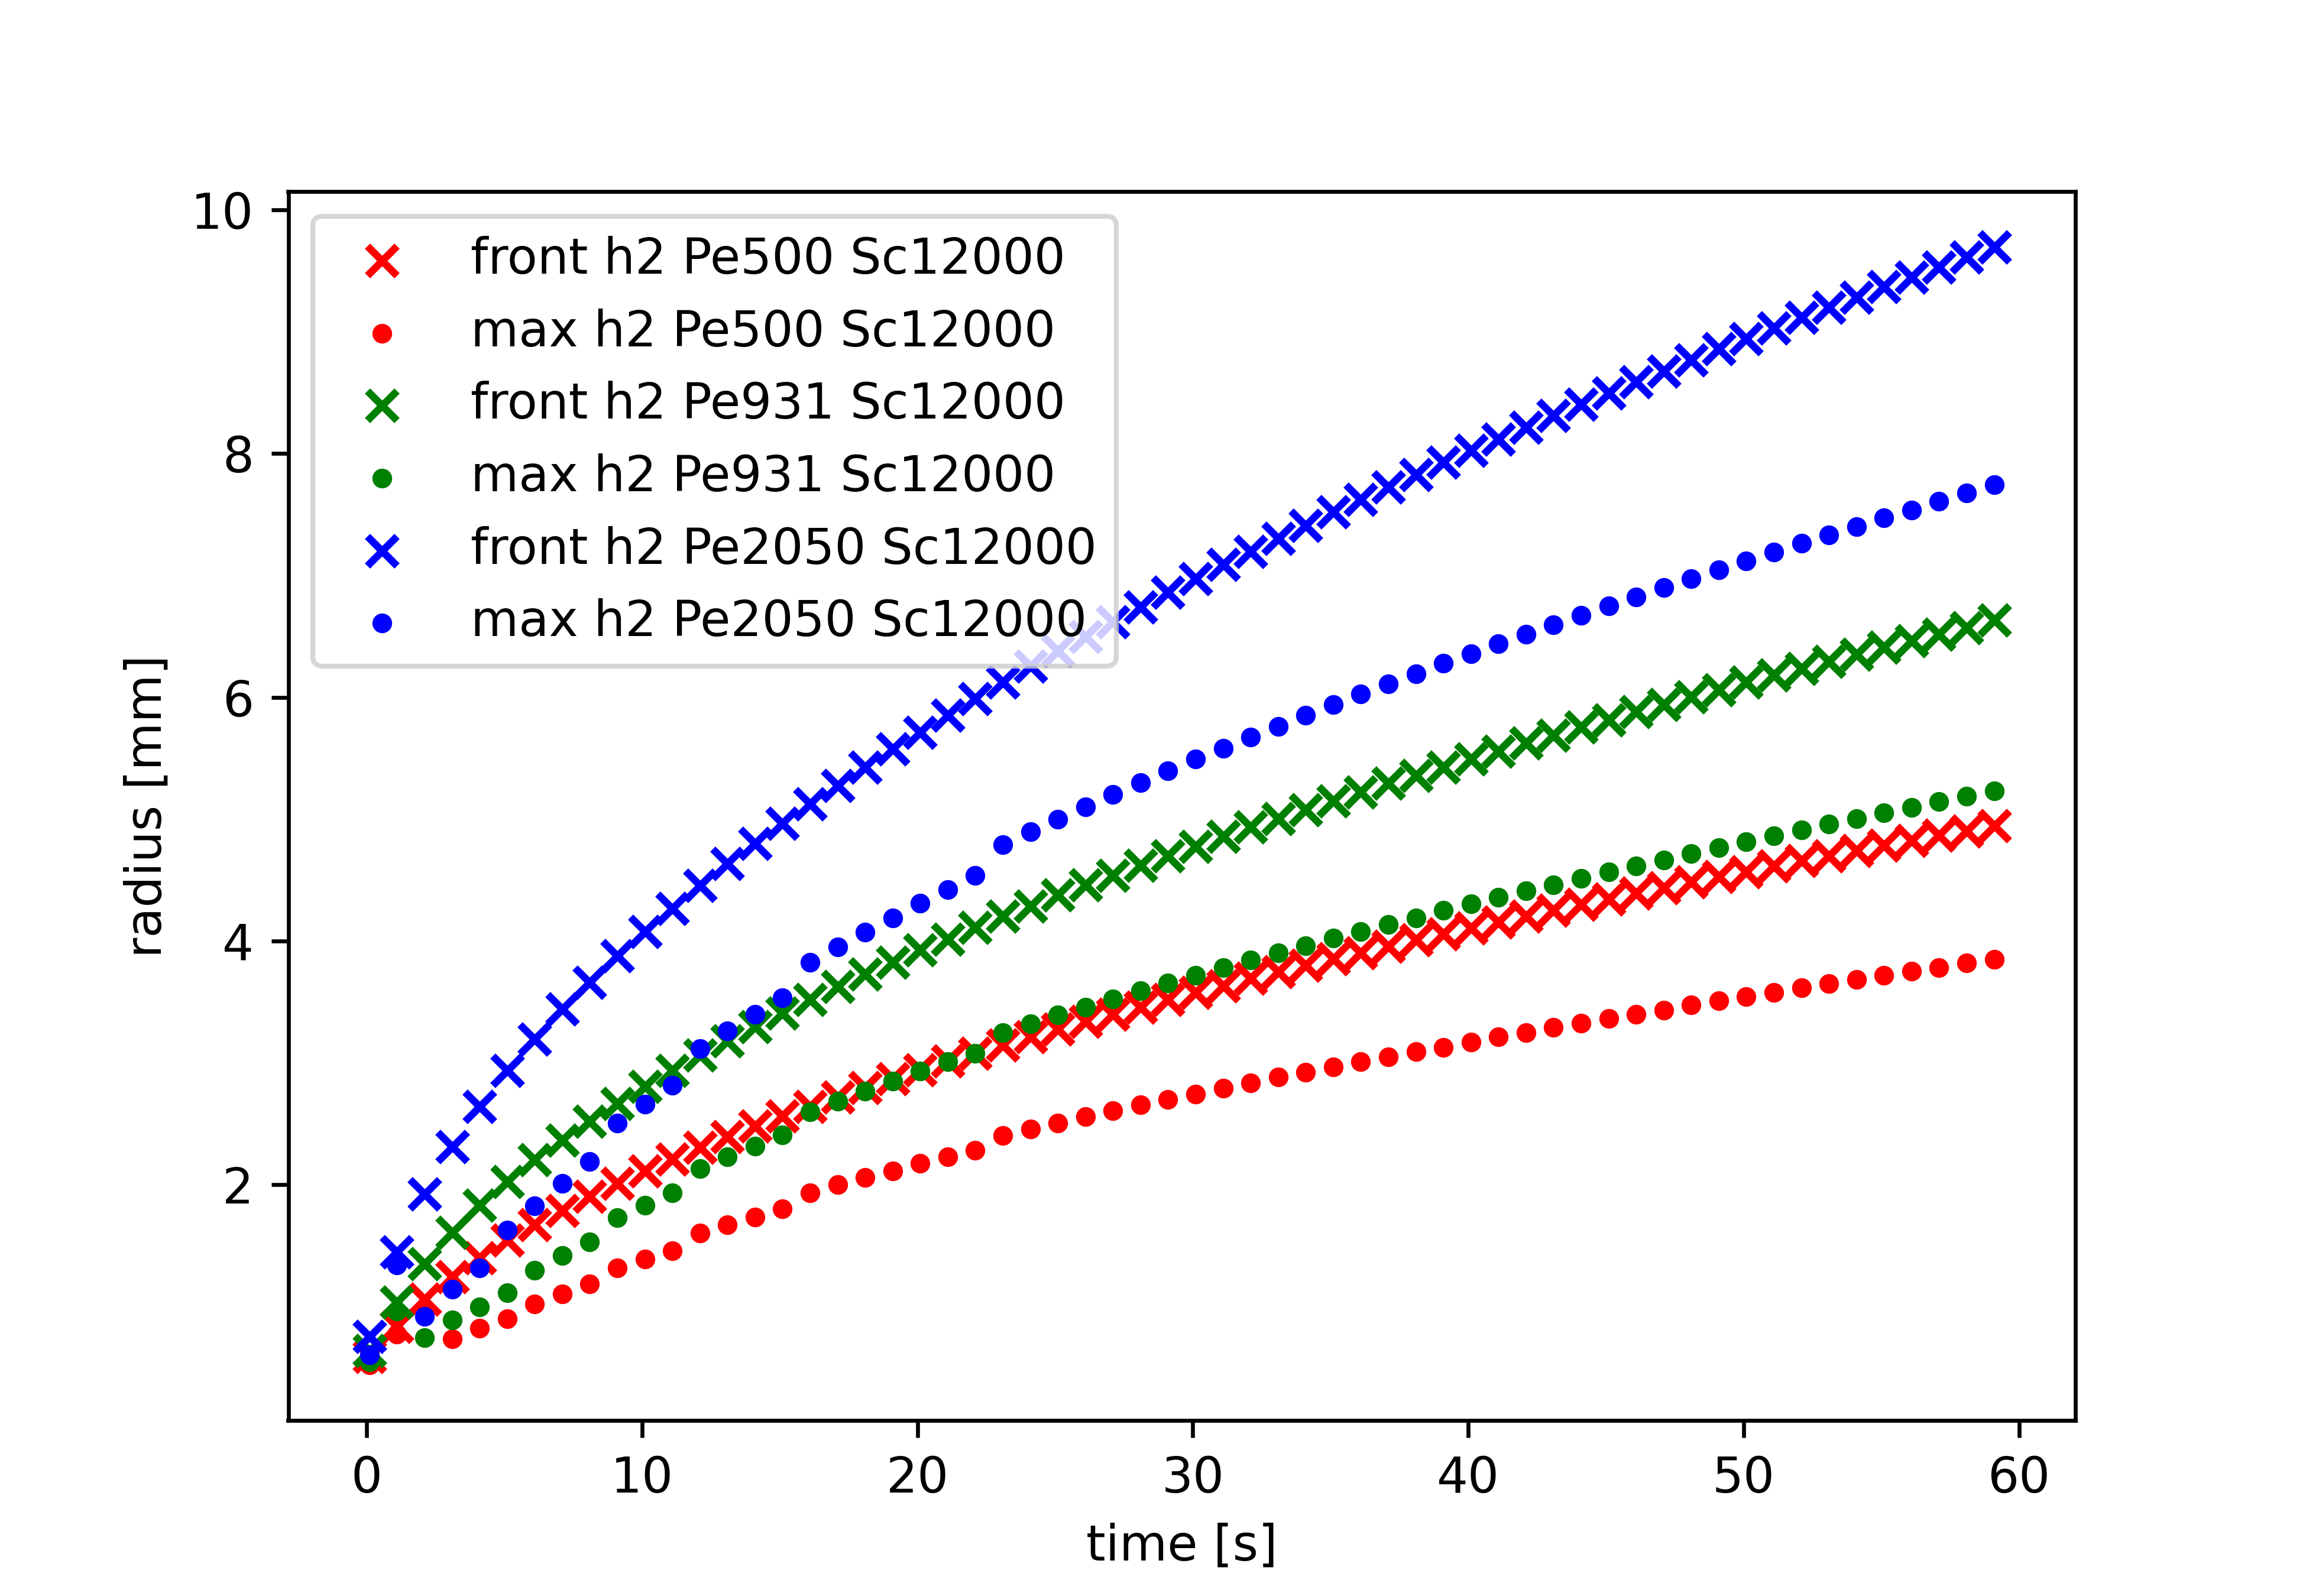
\includegraphics[width=.9\linewidth]{front_pos_h2_Sc12000}
	\caption{front positions for  h = 0.2mm Sc = 12000
	\label{fig: front_pos_h2_Sc12000}}
\end{figure}
For a Schmidt number of 12000 the values for $r_{\text{front}}$ and $r_{\text{max}}$ do show a similar behaviour on a principle level. The $r_{\text{front}}$ positions travel speed decays over time and seems to follow an approach close to a square root function. The values for $r_{\text{max}}$ do show the same behaviour but are always at lower radial values than the front values $r_{\text{front}}$.
\begin{figure}[htb]
	\centering
	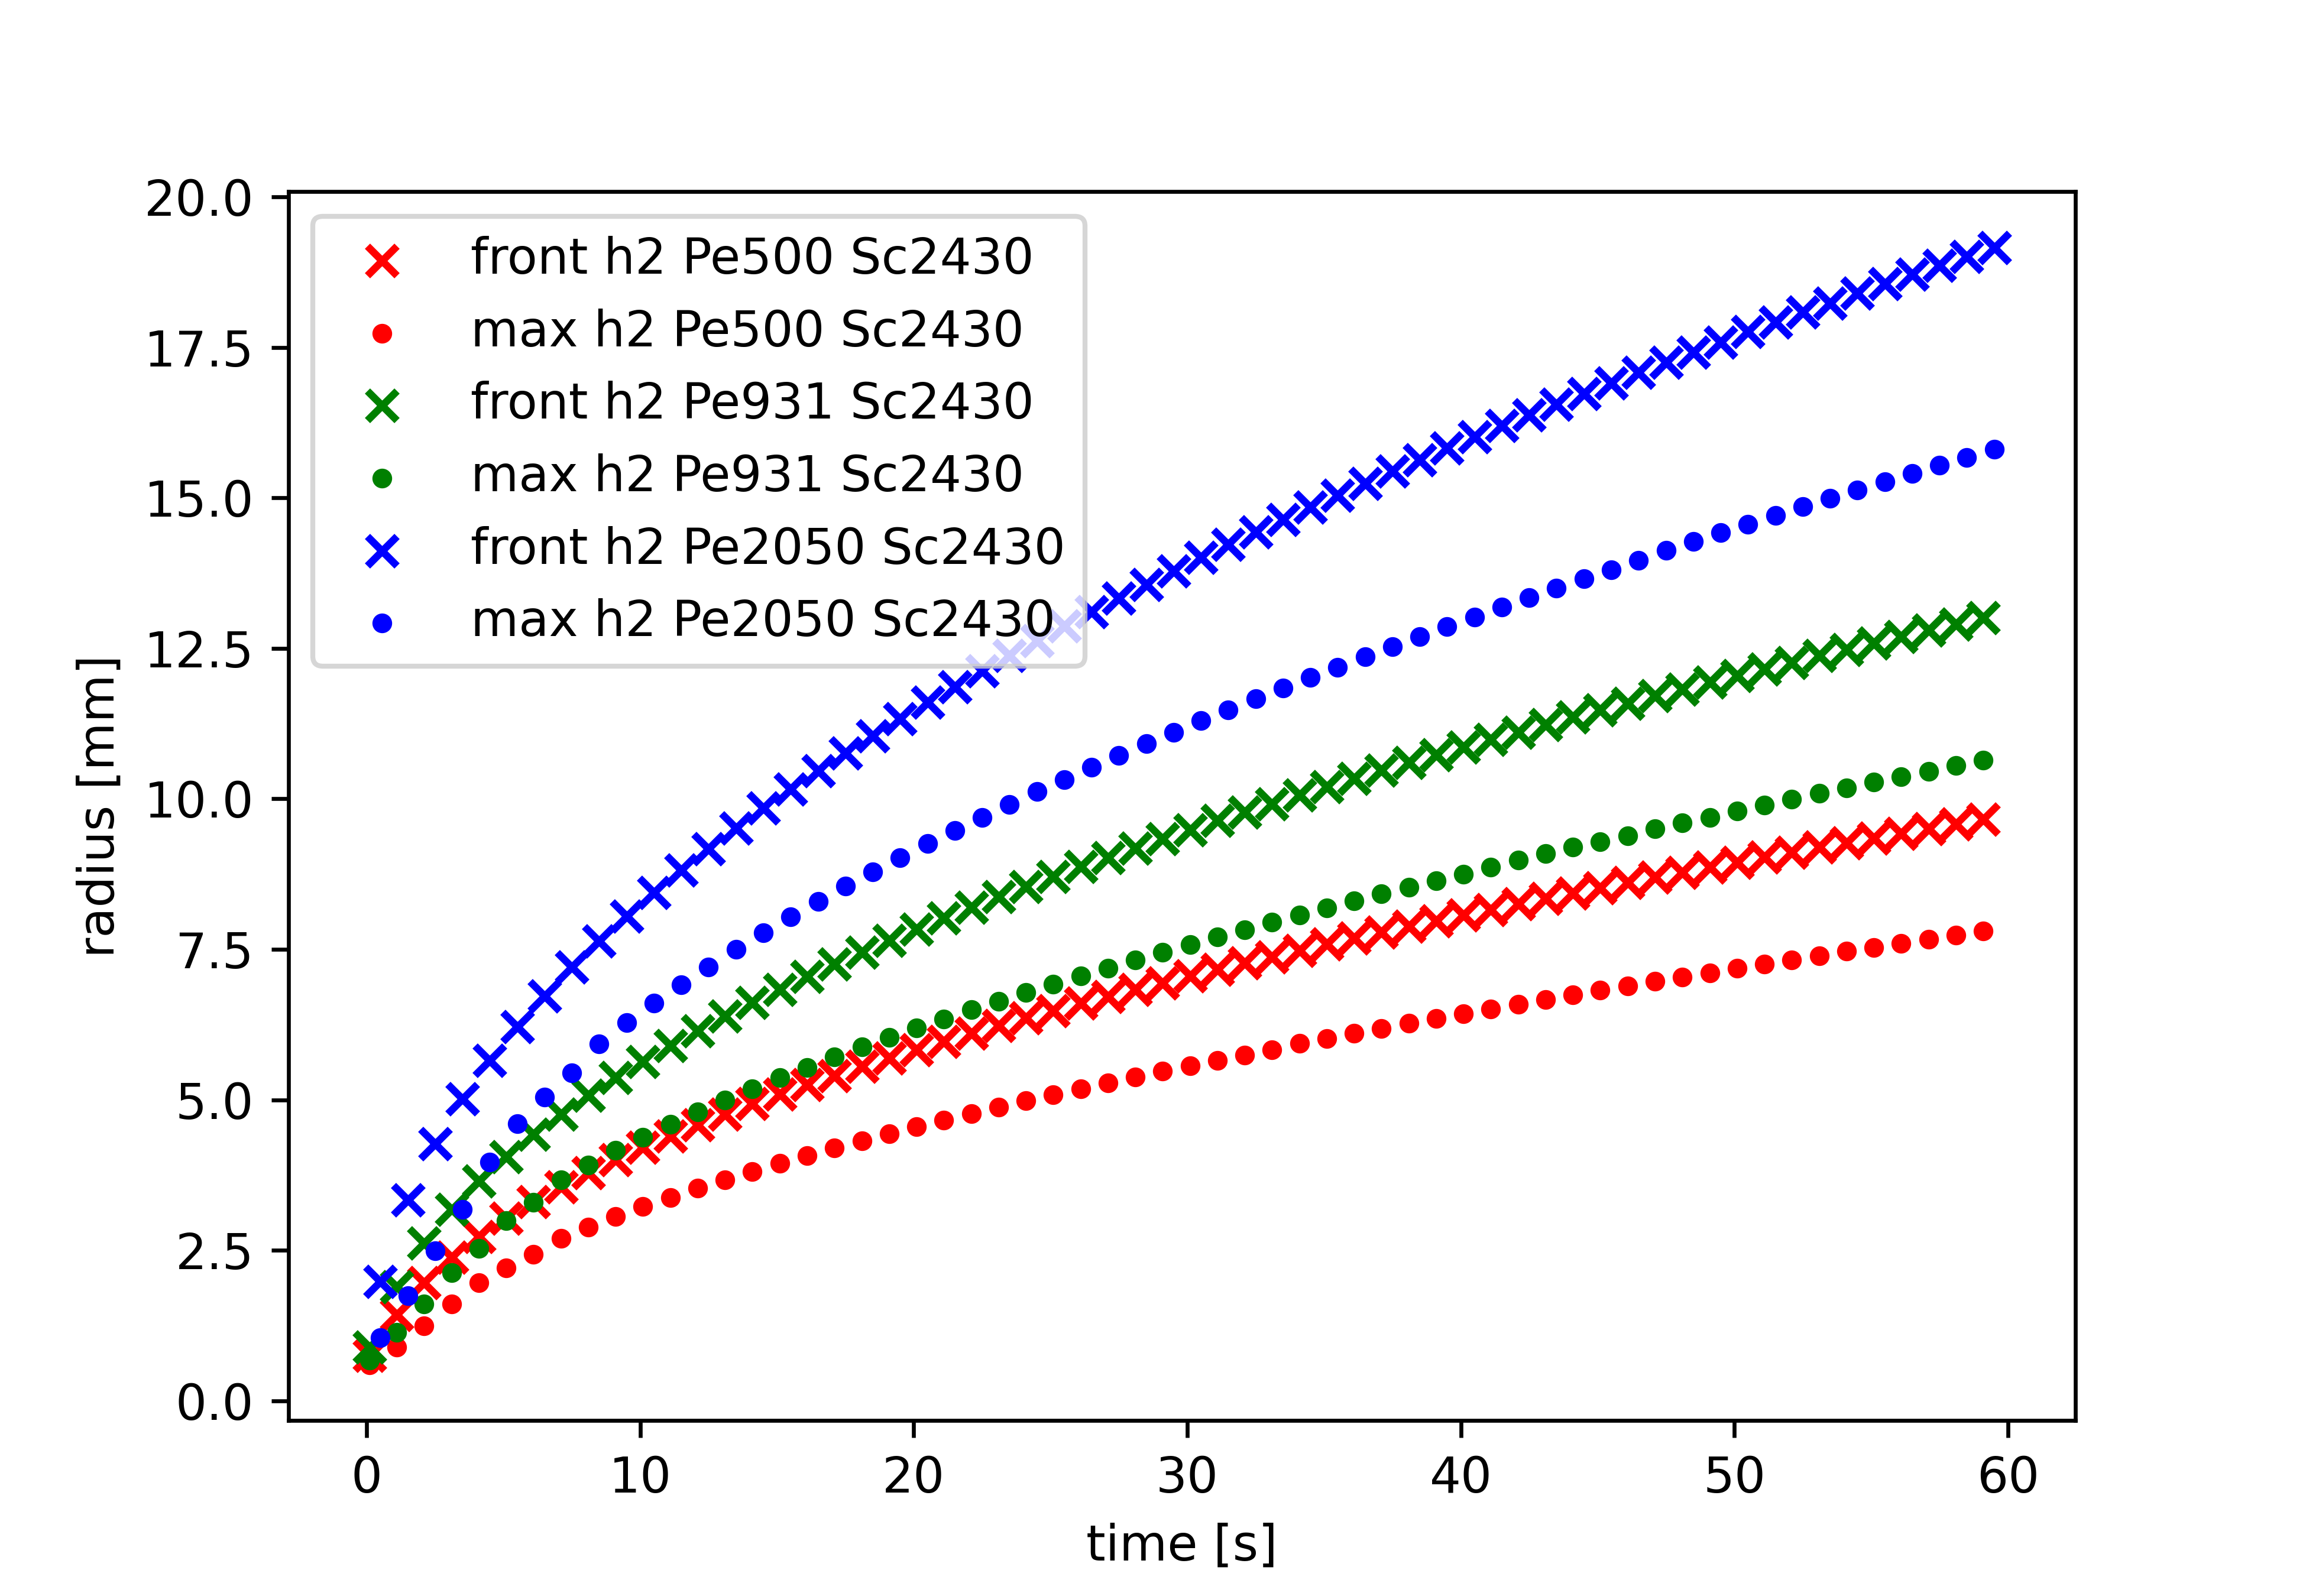
\includegraphics[width=.9\linewidth]{front_pos_h2_Sc2430}
	\caption{front positions for  h = 0.2mm Sc = 2430
	\label{fig: front_pos_h2_Sc2430}}
\end{figure}

The described behaviour is the same for the cases with Sc = 2430.

The $r_{\text{front}}$ and $r_{\text{max}}$ positions travel faster for higher Peclet numbers, which can be explained by the different input velocities. With decreasing inlet velocity the difference between the fronts front and maximum position at later time steps decreases. The decrease is more significant for cases with higher Peclet numbers. For cases with lower Peclet numbers the distance between  $r_{\text{front}}$ and $r_{\text{max}}$ at the end is approximately the same. This can be seen in \autoref{fig: front_pos_h2_Sc2430} when looking at the plots for Pe = 500 and comparing it with the ones for Pe = 931. For these cases, due to their lower absolute inlet velocity, the distance between the front's front and maximum is smaller and doesn't change that much if the velocity is risen or lowered.

When comparing the plots for Schmidt number 2430 with the one for a Schmidt number of 12000 it can be observed that all fronts travel nearly double the distance within the same time of 60 seconds. This can be explained mainly by the lower diffusion coefficient for the higher Schmidt number case. The diffusion coefficient for the lower Schmidt number case is $4 \text{.}11 \cdot 10^{-10} \left[ \frac{\mathrm{m^2}}{\mathrm{s}} \right]$ and the one for the higher Schmidt number case is $1\text{.}0 \cdot 10^{-10} \left[ \frac{\mathrm{m^2}}{\mathrm{s}} \right]$. In addition to the global Peclet number introduced in \autoref{eqn: Pe} a local one can be defined using \autoref{eqn: Pe local}.
\begin{equation}
	Pe_{\text{local}} = \dfrac{h \cdot u(x,r)}{D}
	\label{eqn: Pe local}
\end{equation}
In this equation the local velocity $u(x,r)$ at the coordinates $x$ and $r$ is used instead of the inlet velocity $u$ used within the global Peclet-Number.
Since the velocity magnitude decreases very quickly for a axisymmetric reactor (see \autoref{fig: field_example}) $Pe_{\text{local}}$ does show the same behaviour as they are directly linked to each other. As the Peclet number is defined as the advective transport rate divided by the diffusive transport rate a low local Peclet number means that diffusion plays a more and more significant role while the front travels through the reactor. 

The diffusion coefficient has not only an influence on the front's position. The front's width is affected by diffusion as well. The fronts width will be analysed within the following section.

\section{Front Widths}

The fronts width behaviour is quite different for each reactor geometry so each one will be looked at starting with the smallest gap height of 0.2mm. The front widths for that geometry are shown in \autoref{fig: front_width_h2_Sc12000} and \autoref{fig: front_width_pos_h2_Sc2430} for each investigated Schmidt number.
\begin{figure}[htbp]
	\centering
	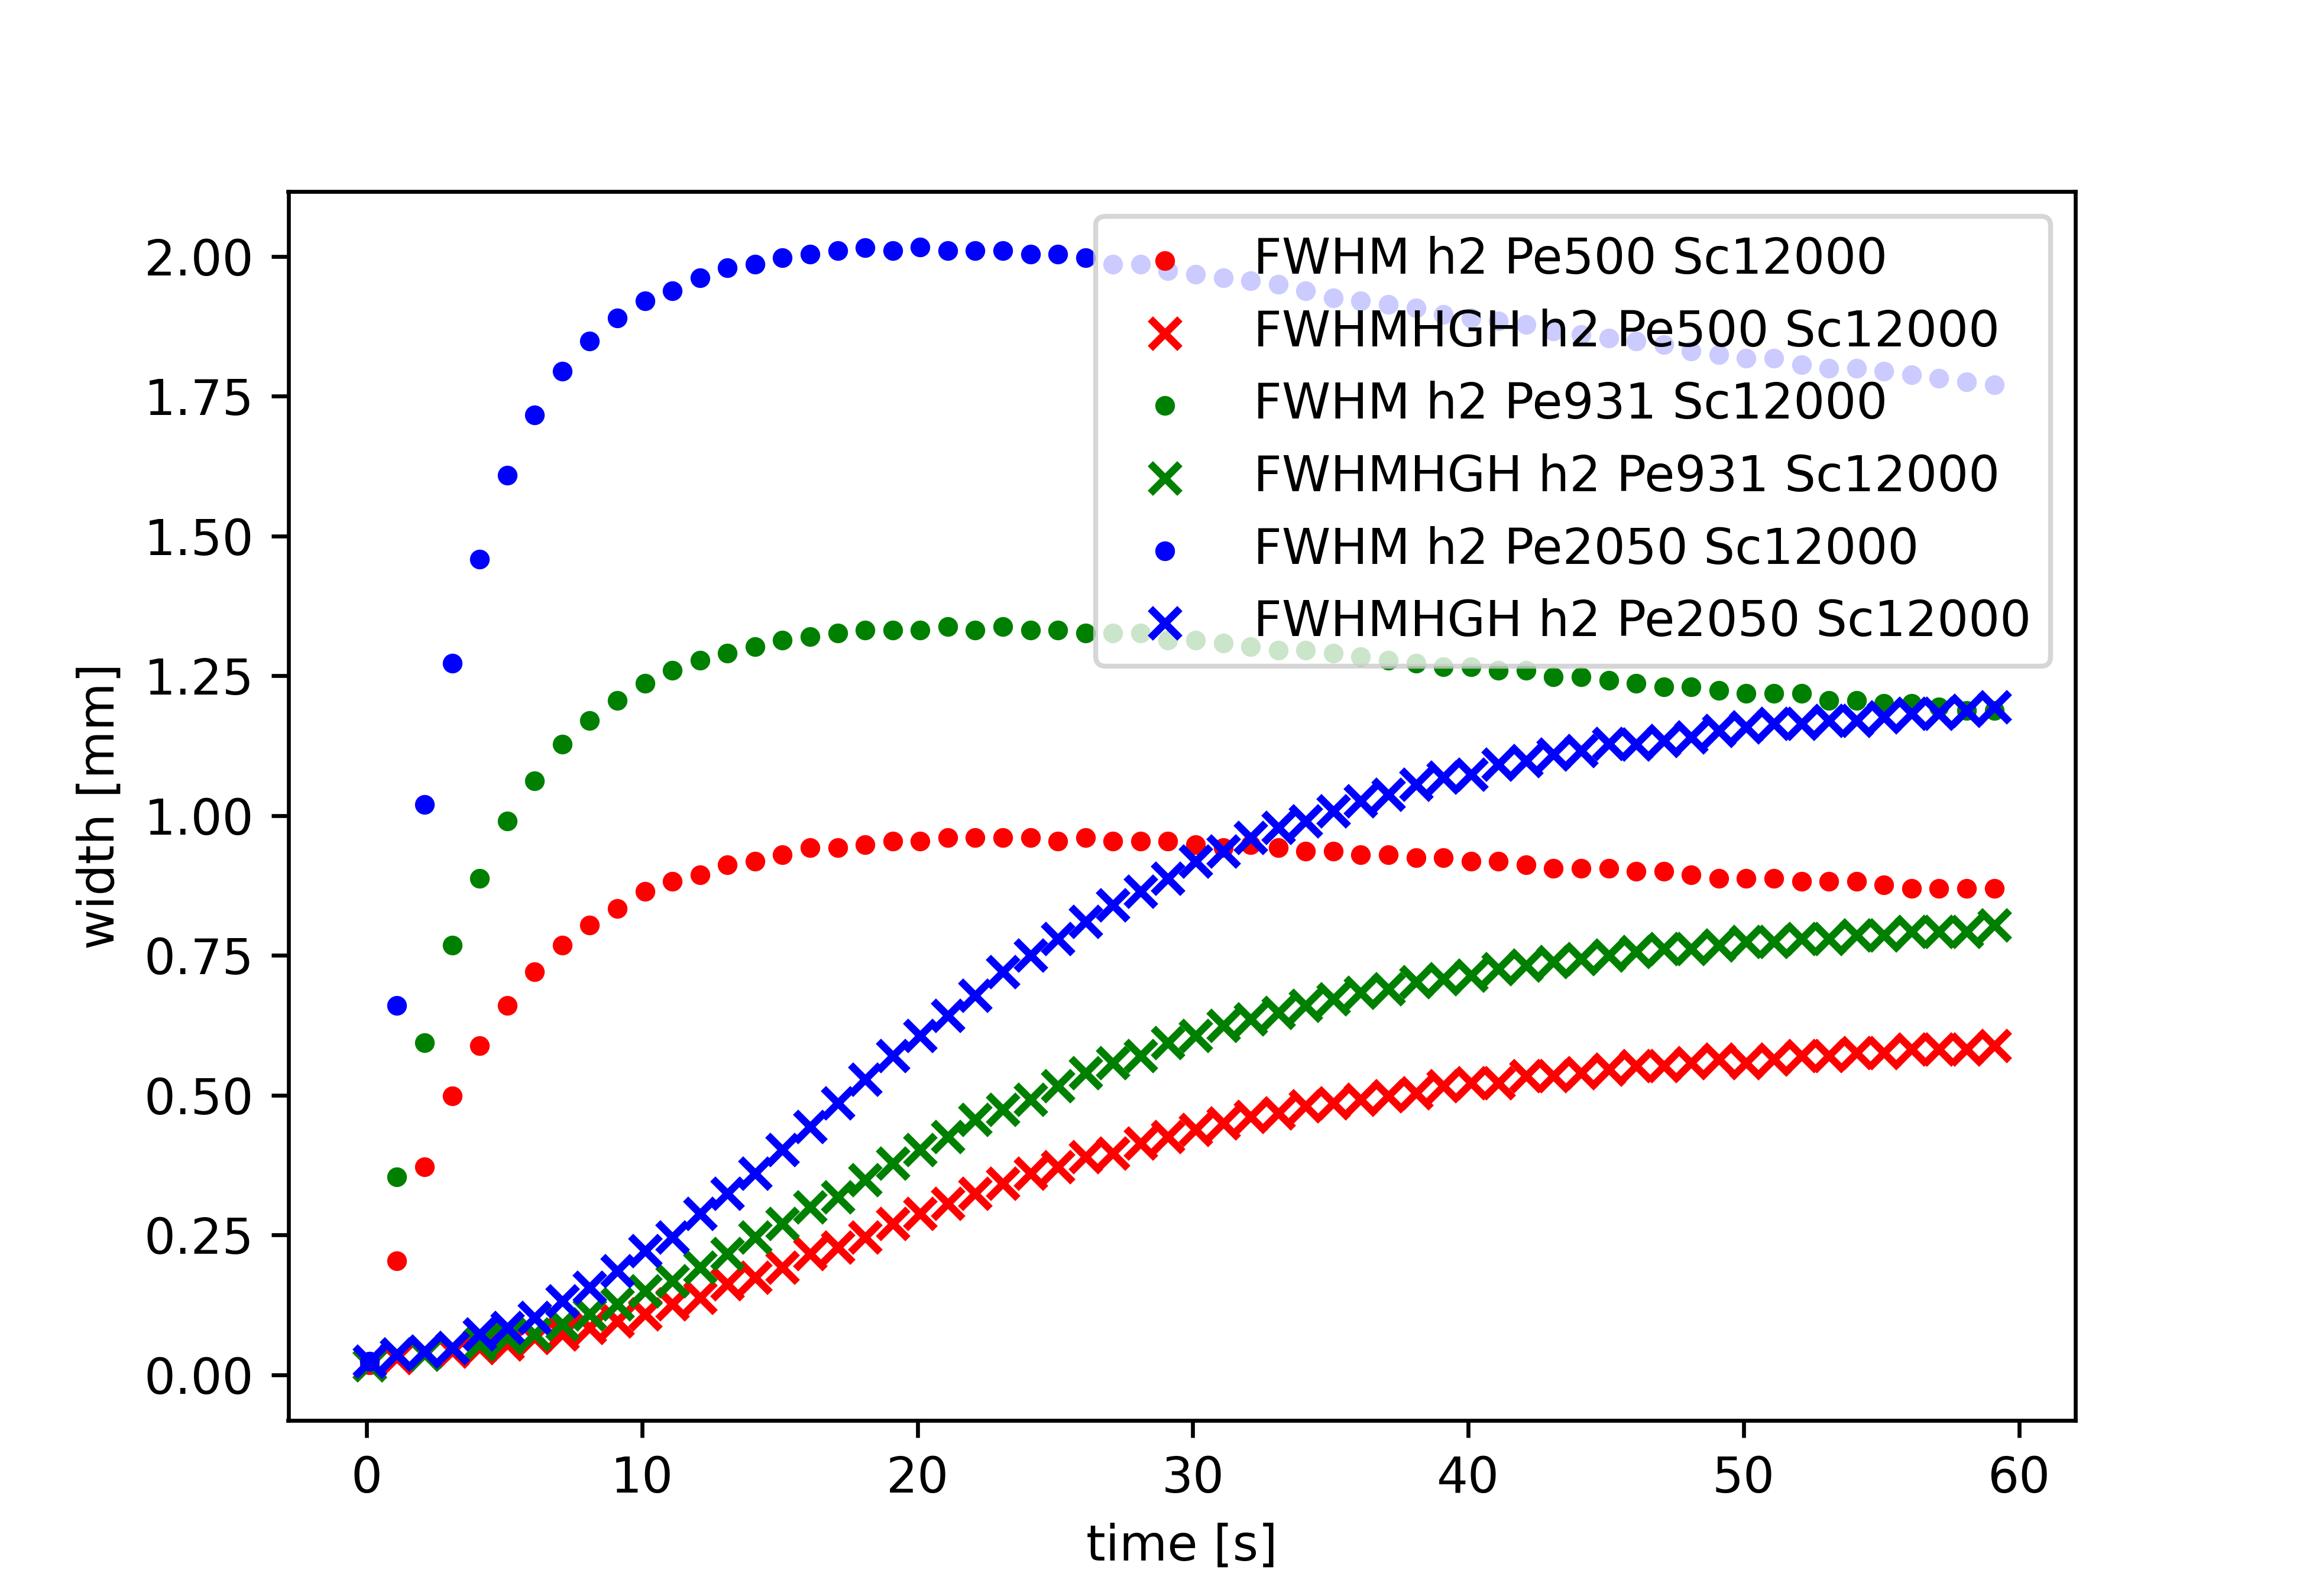
\includegraphics[width=0.8\linewidth]{front_width_h2_Sc12000}
	\caption{front widths for  h = 0.2mm Sc = 12000
	\label{fig: front_width_h2_Sc12000}}
\end{figure}
Within the plot for the Schmidt number of 12000 it can be seen that the width using the gap averaged product concentration data (FWHM) starts growing fast within the first seconds. After that the widths growth slows down and the width reaches its maximum value. When the maximum has been reached the width starts shrinking slowly towards a final constant value. The FWHMGH does show a different behaviour. Its growth starts slow within the first few seconds and then starts to follow a square root like approach towards a final constant value. The widths do reach higher values for higher Peclet numbers.
\begin{figure}[htbp]
	\centering
	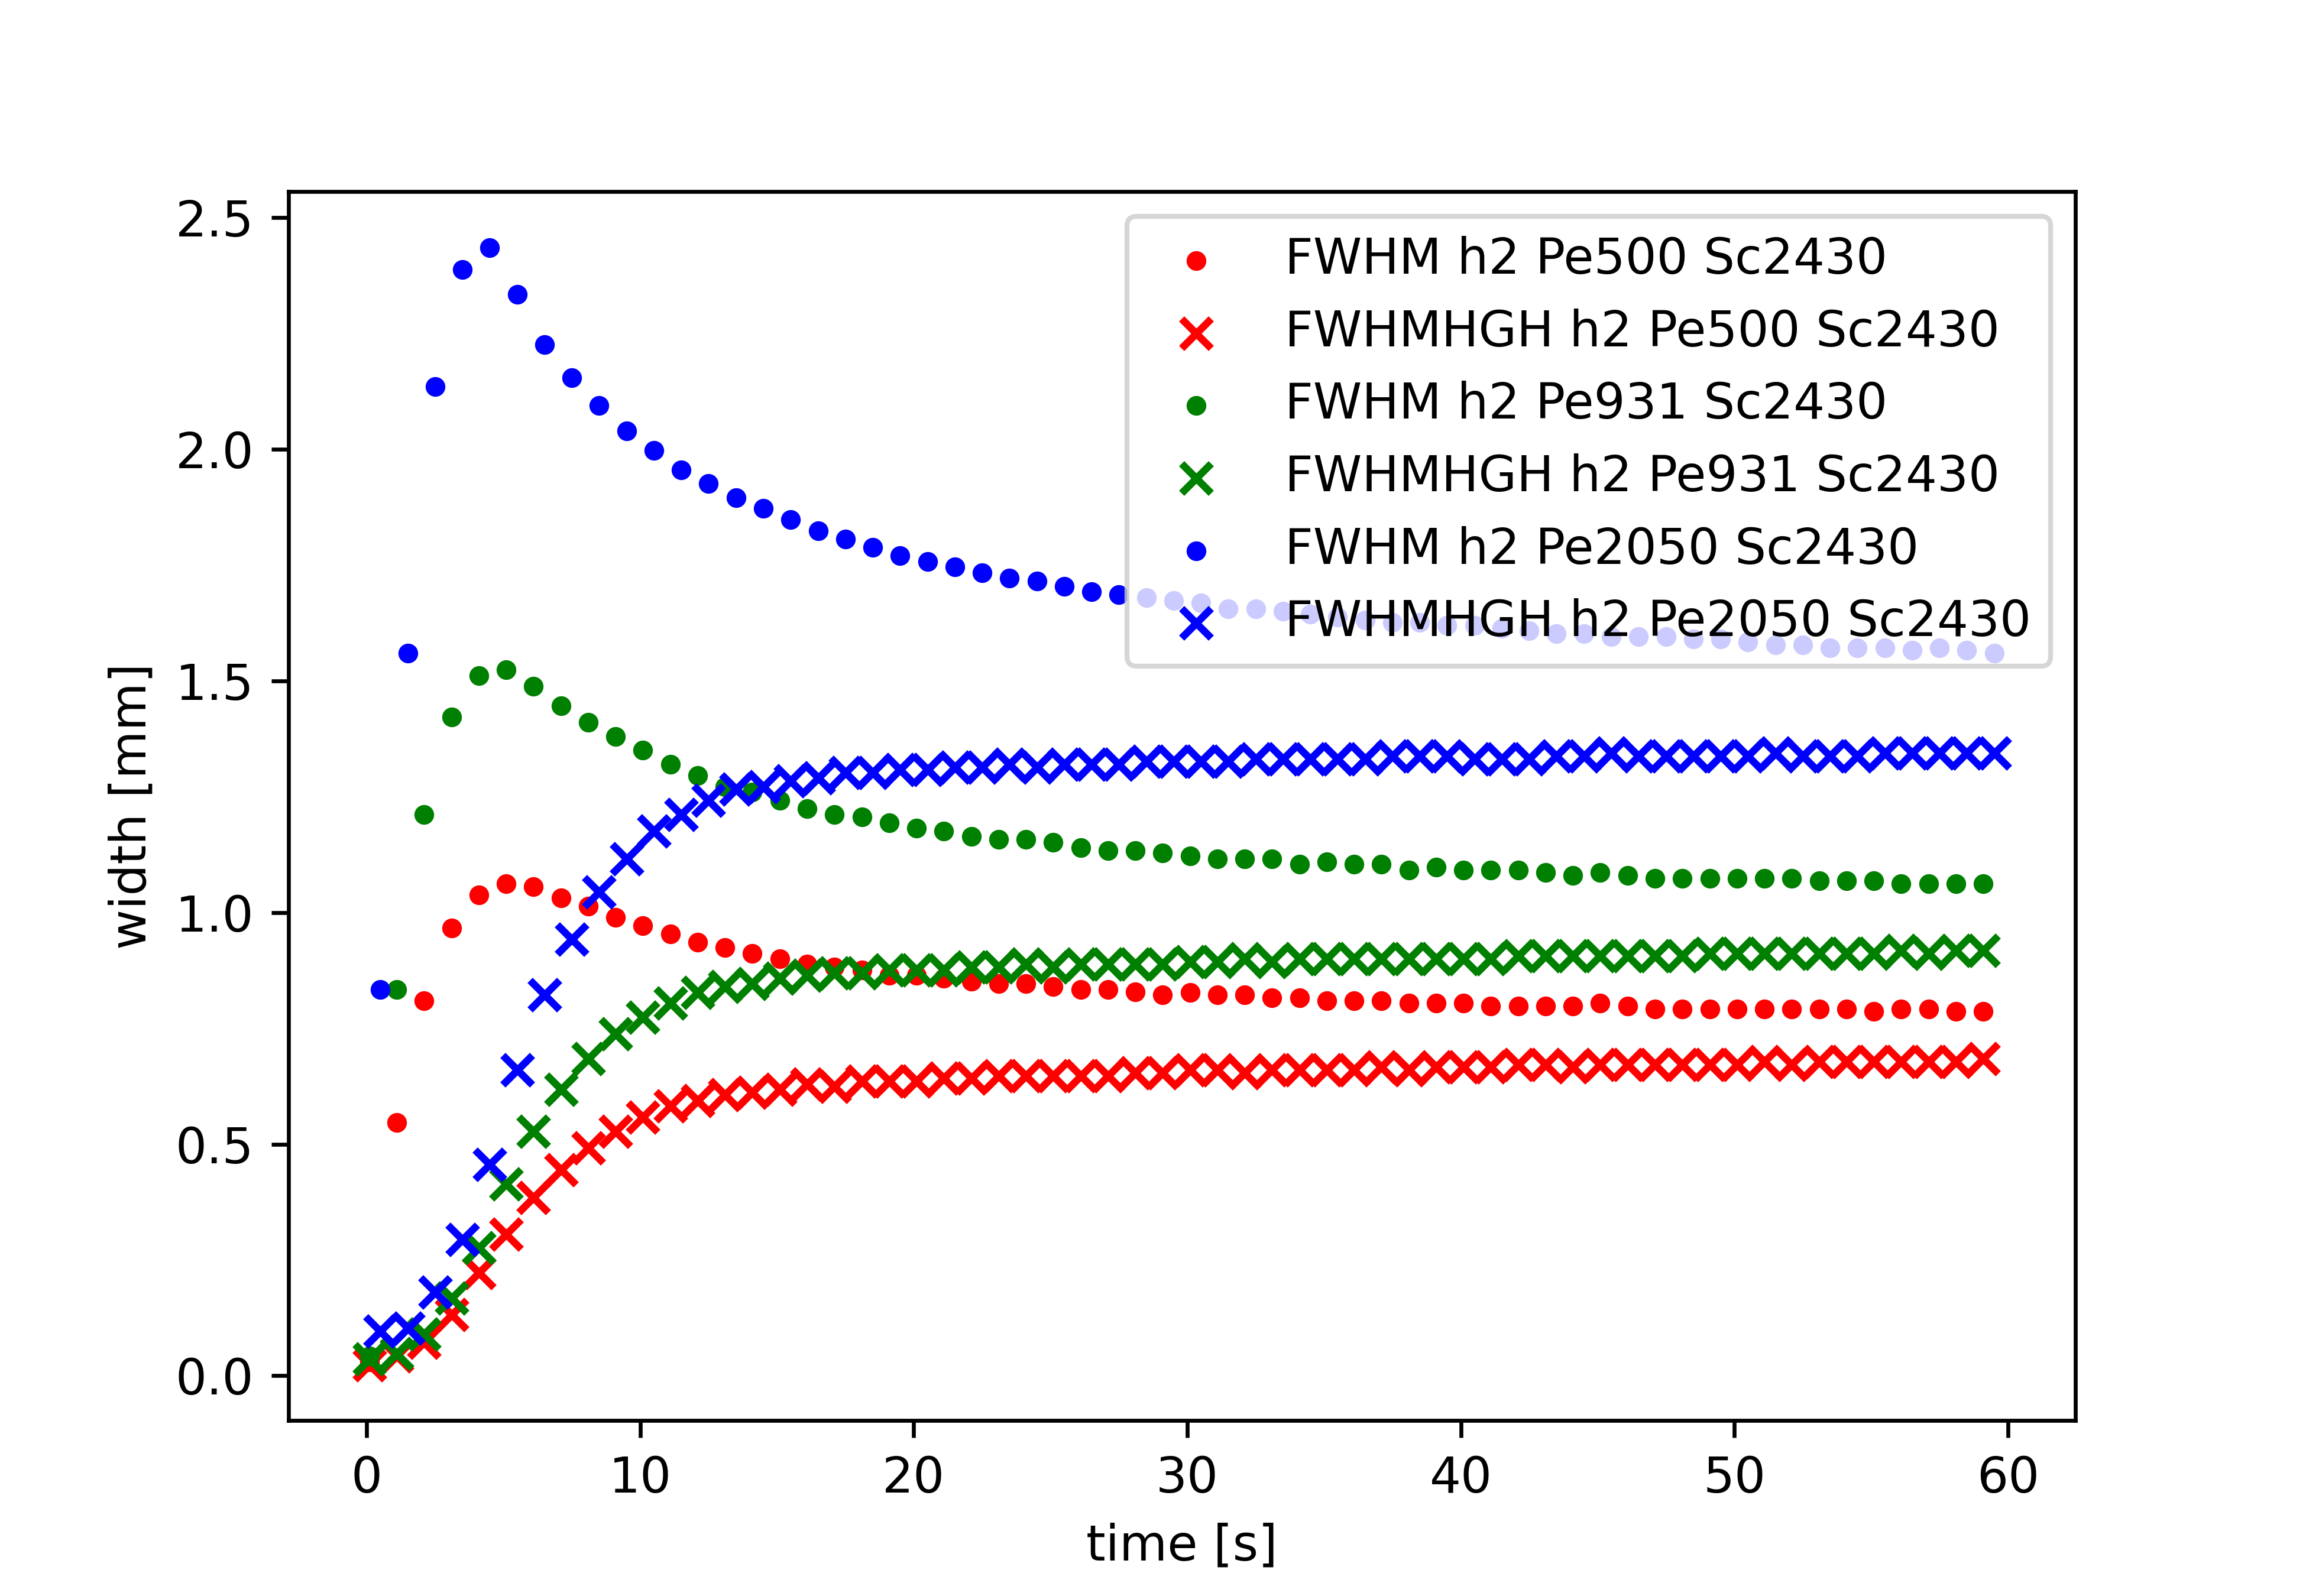
\includegraphics[width=0.8\linewidth]{front_width_h2_Sc2430}
	\caption{Front widths for  h = 0.2mm Sc = 2430}
	\label{fig: front_width_pos_h2_Sc2430}
\end{figure}
For the case with a Schmidt number of 2430 the width's growth in the beginning is even fast compared to case with the higher Schmidt number. This faster growth can be seen for both the FWHM as well as the FWHMHGH. The decrease after the front has reached it's maximum value is more visible for the lower Schmidt number cases. From these cases it can be seen that both calculated widths seem to be driven towards the same value for later times. The same behaviour is expected to happen at later times for the simulation in the cases with Sc = 12000 which no results are calculated for.

The reason for initial high growth is that the front is near the inlet an new reactants are constantly available due to the high flow rate in that region. In addition to that the front's width has low values so the distance both reactants $A$ and $B$ need to travel to reach each other to form the product $C$ is low. In the beginning the front's shape can be represented by a straight line which gets distorted over time as visible in \autoref{fig: shape_examp}a. This distortion creates new surface area for the reaction to take place in addition the area generated by the front's spreading in a radial reactor.

The strive towards the same value for both the FWHM and the FWHMHGH at later times can be explained by the fronts shape. In \autoref{fig: pos_h2_late} the product concentration field is shown at the time of 60 seconds for the case with a Peclet number of 500 and a Schmidt number of 2430.
\begin{figure}[htb]
	\centering
	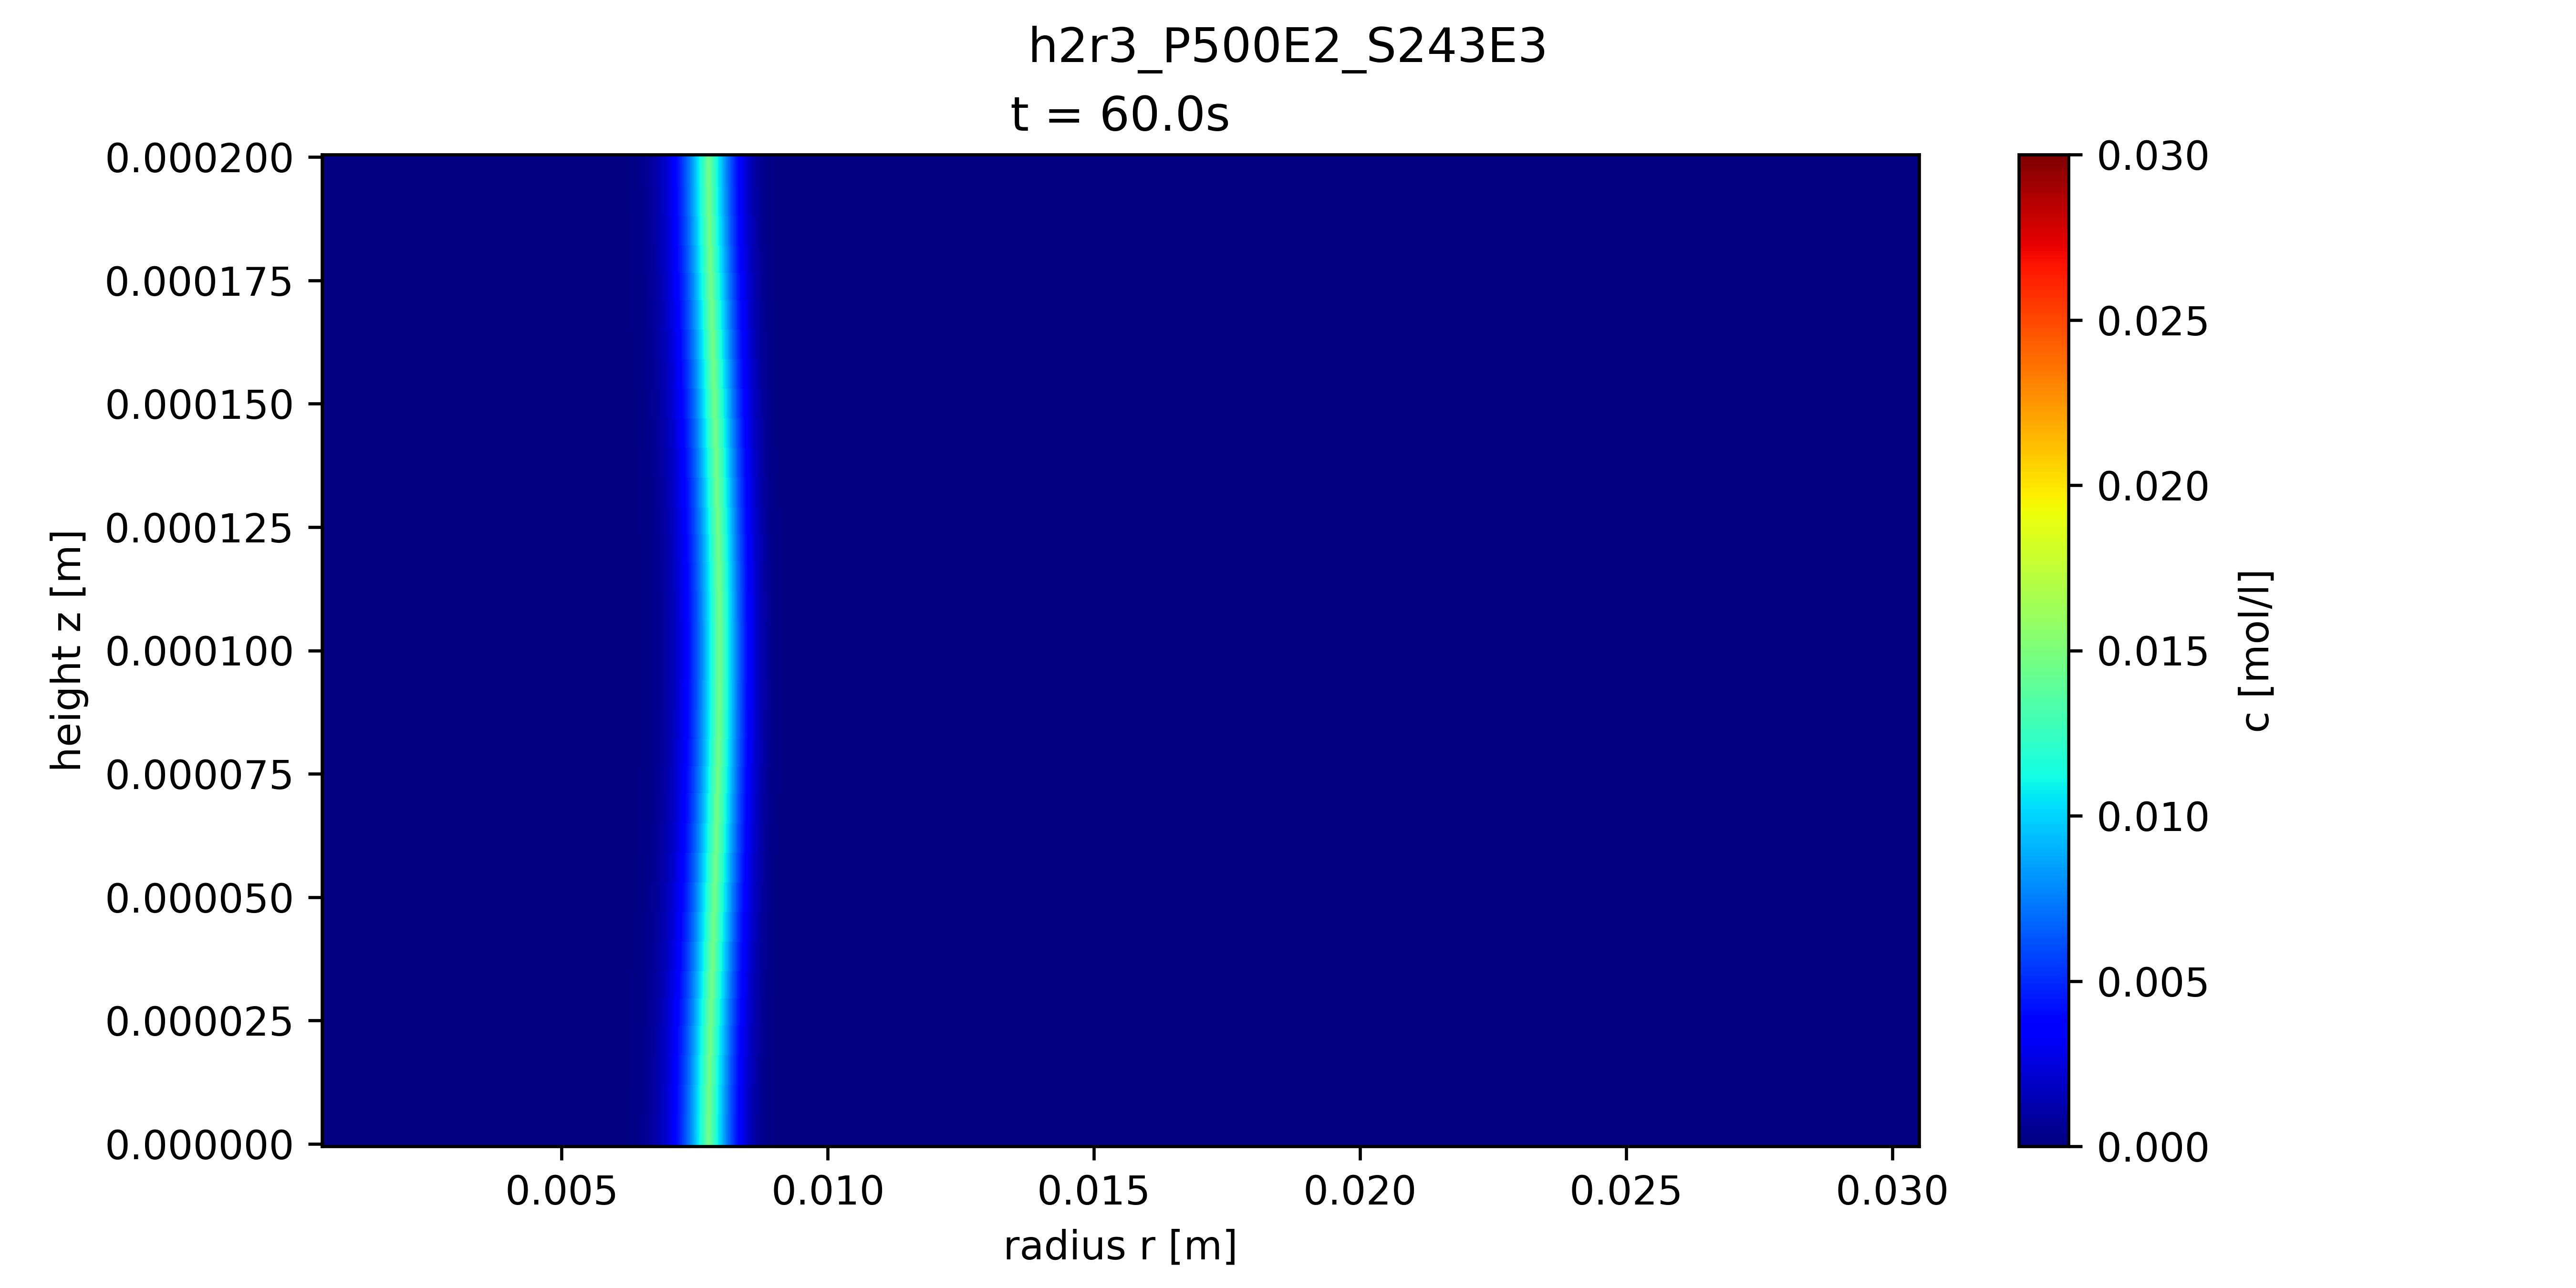
\includegraphics[width=\textwidth]{img_gif_h2r3_P500E2_S243E3_60,0 }
	\caption{Front shape for h=0.2mm Pe = 500 Sc = 2430 at 60 seconds}
	\label{fig: pos_h2_late}
\end{figure}
When the front reaches the shown shape the difference between the width using the FWHM method and the middle with decreases. As shown in \cite{comolli2021dynamics} the reaction decays until the spreading of front by diffusion forms an equilibrium with the reactants consumed by the reaction.

Another reason for the decay could be, that maximum value changes so the positions the widths are taken from do change as well. In \autoref{fig: plot_h2_widths} the gap averaged concentration plots are shown for a time of 2 seconds which is in the phase of width growth, a time of 5 seconds which is close to the maximum and a time of 18 seconds which is near the end of the decaying phase. From this plot it can be seen that the curvature does change over time. It widens at first when comparing the curves for $t = 2s$ with $t = 5s$ and then narrows down. In addition to that the maximum value raises, since more product is generated over time. With the maximum value raising, the position of $0\text{.}5 \cdot c_{C,max}$ changes as well towards the more narrow section of the curve. 
\begin{figure}
	\centering
	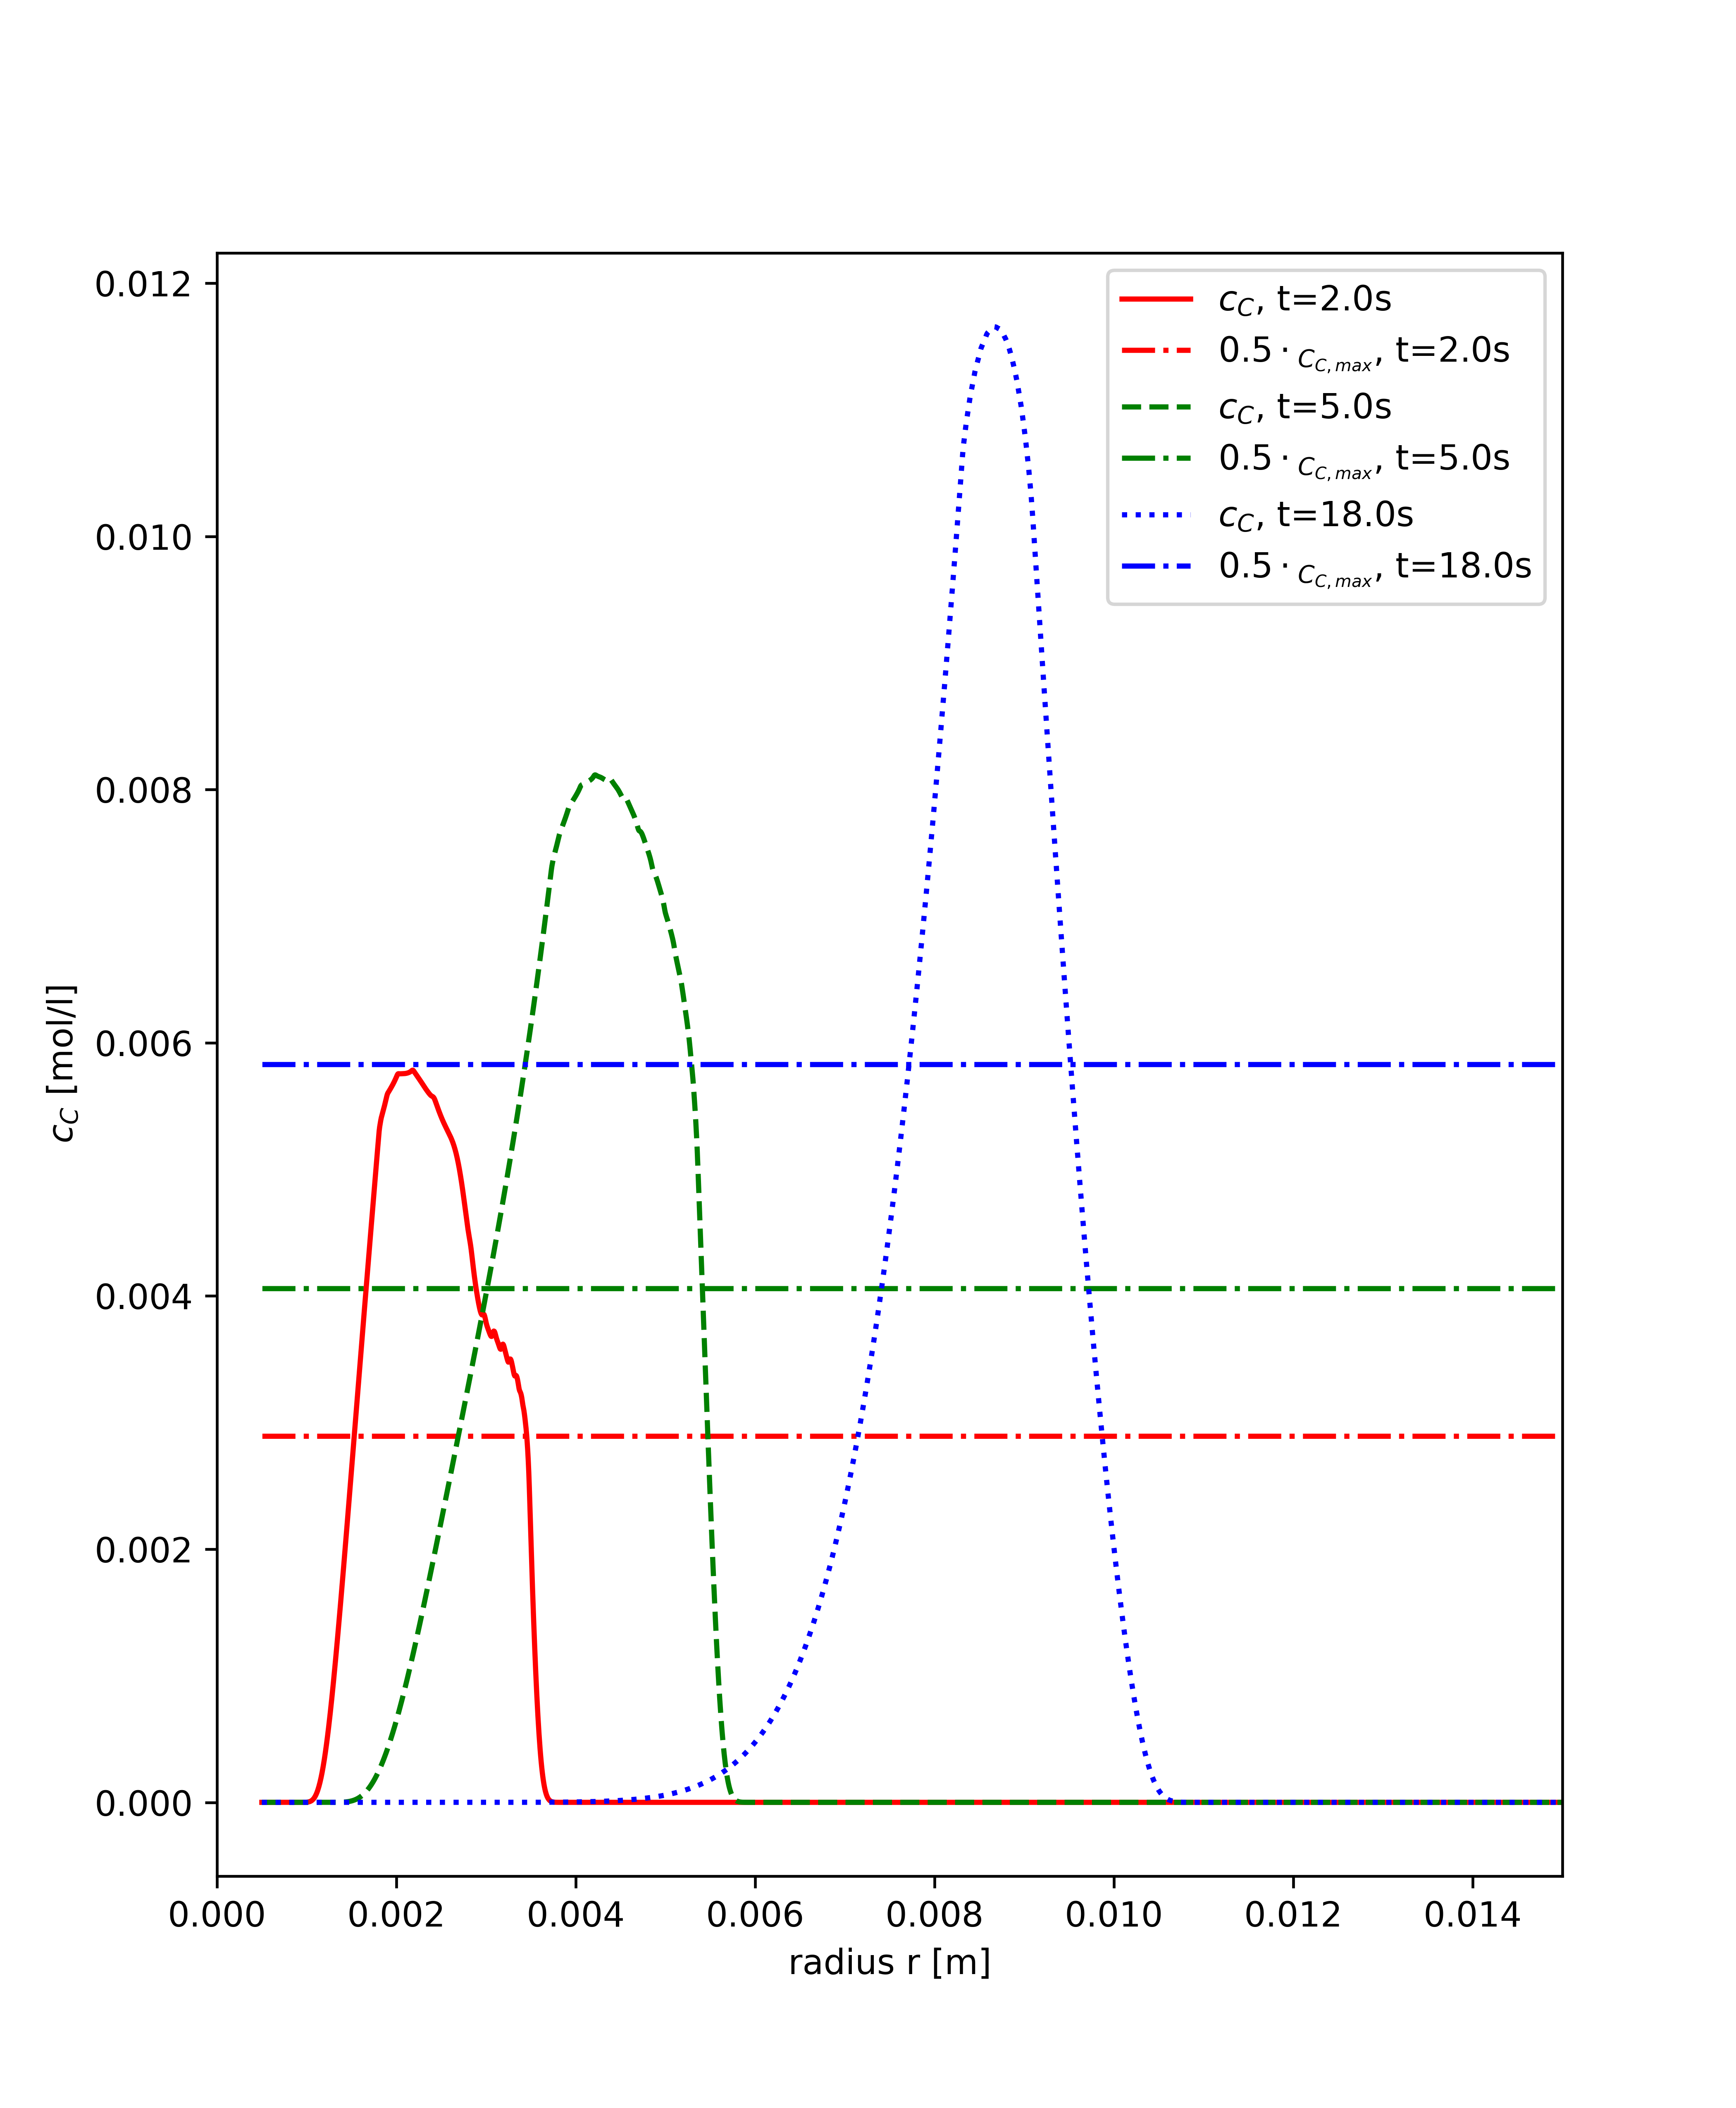
\includegraphics[width=\textwidth]{plot_h2r3_P205E3_S243E3_concentration-fluid_c}
	\caption{Product concentration plots for h = 0.2mm  Pe = 2050 Sc = 2430 for different times}
	\label{fig: plot_h2_widths}
\end{figure}

When comparing both Schmidt number plots with each other it can be observed that the final widths value seems to be independent of the Schmidt number for a gap height of 0.2mm. For this gap height that is true for both the FWHM and the  FWHMHGH. The results from the 0.4mm case also support this assumption for the FWHM. To get clearer evidence if the assumption is correct more Schmidt numbers need to be investigated and the simulations should be run for longer durations. These longer durations are also needed to get a clearer picture on how the FWHMHGH behaves at later stages of the simulation run.

Another observation that can be made is that the time the width reaches its maximum value and the maximum value itself is strongly influenced by the Schmidt number. For the lower Schmidt number of 2430 a clear peak is visible for all Peclet numbers. This forming peak seems to be expected because the diffusion coefficient for the case with the higher Schmidt number of 12000 is lower than the one for the lower Schmidt number of 2430. A lower diffusion coefficient prevents the front from spreading so the width reaches higher values.
\newline

The results for the cases with a gap height of 0.4mm show in most parts a similar behaviour compared to the case with a gap height of 0.2mm.
\begin{figure}[htb]
	\centering
	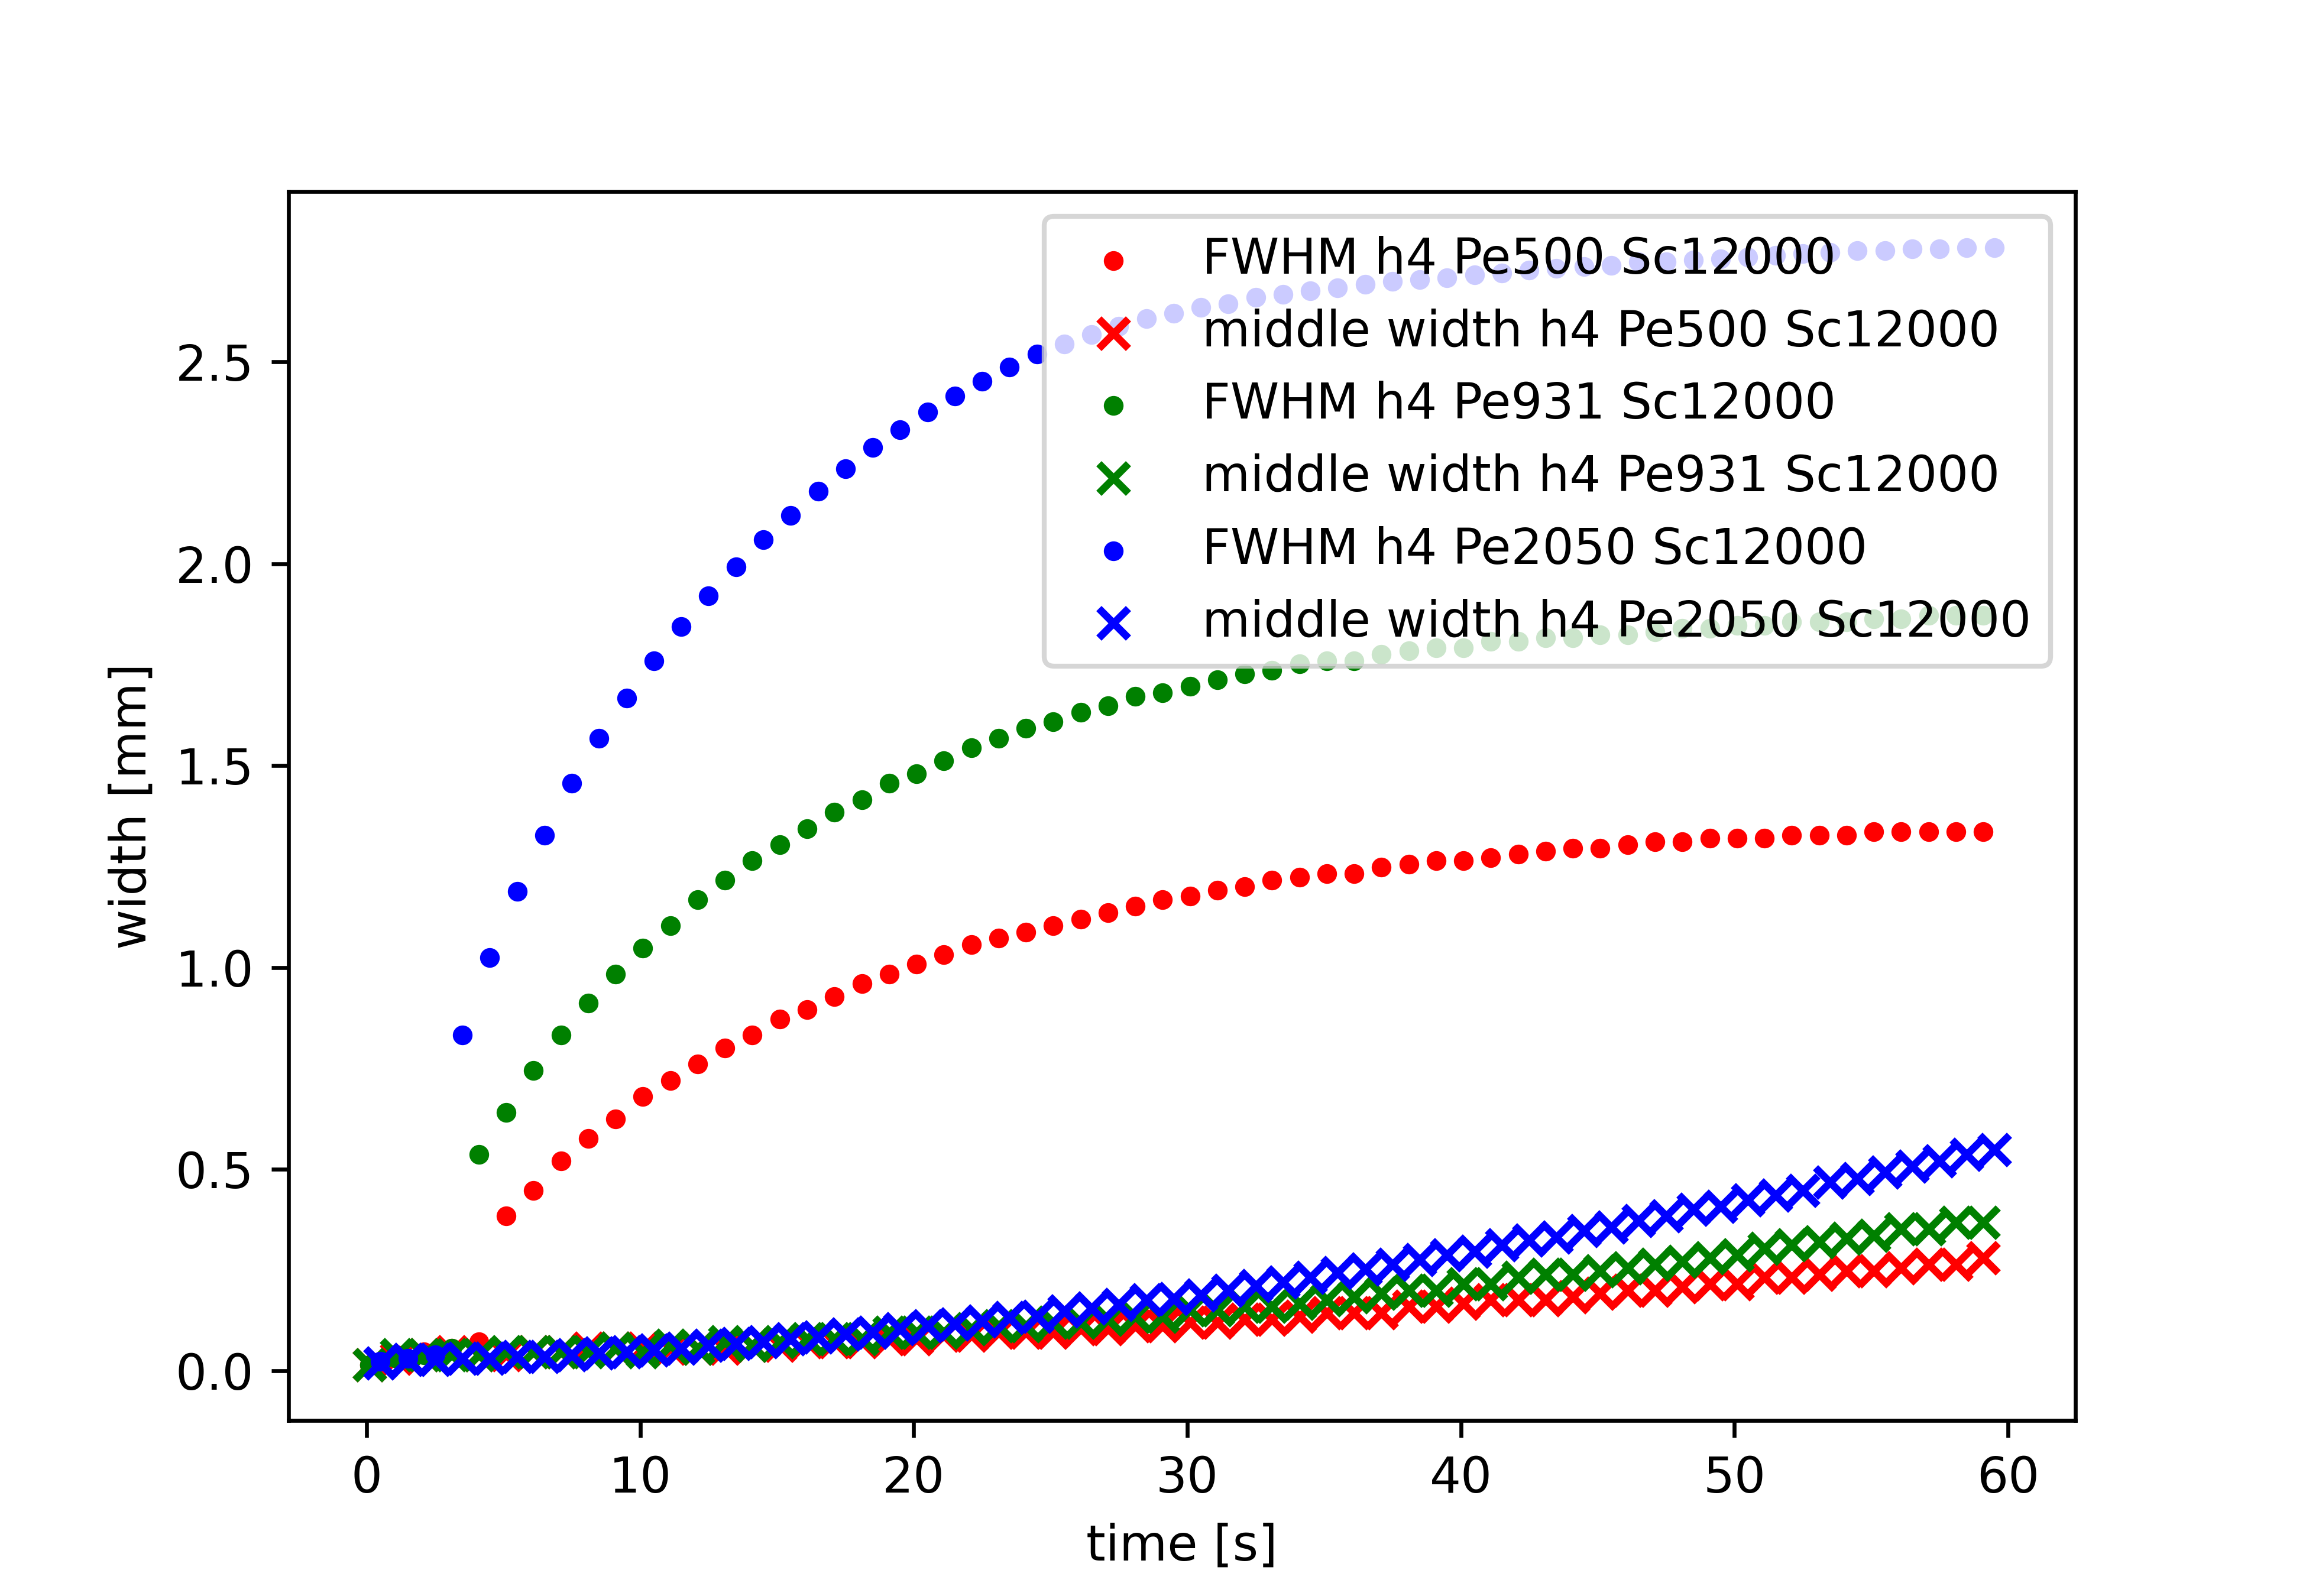
\includegraphics[width=0.85\textwidth]{front_width_h4_Sc12000}
	\caption{front widths for  h = 0.4mm Sc = 12000
	\label{fig: front_width_h4_Sc12000}}
\end{figure}
For the case with the higher Schmidt number of 12000 the FWHM follows a square root like approach for all Peclet numbers. For the first 3 to 5 seconds the FWHM has very low values then starts to grow suddenly. The time the growth starts to happen is higher for lower Peclet numbers. The FWHMHGH has very low values over the hole simulation time for all Peclet numbers investigated. This width's growth seems to slightly increase at later times of around 40 seconds.
\begin{figure}[htb]
	\centering
	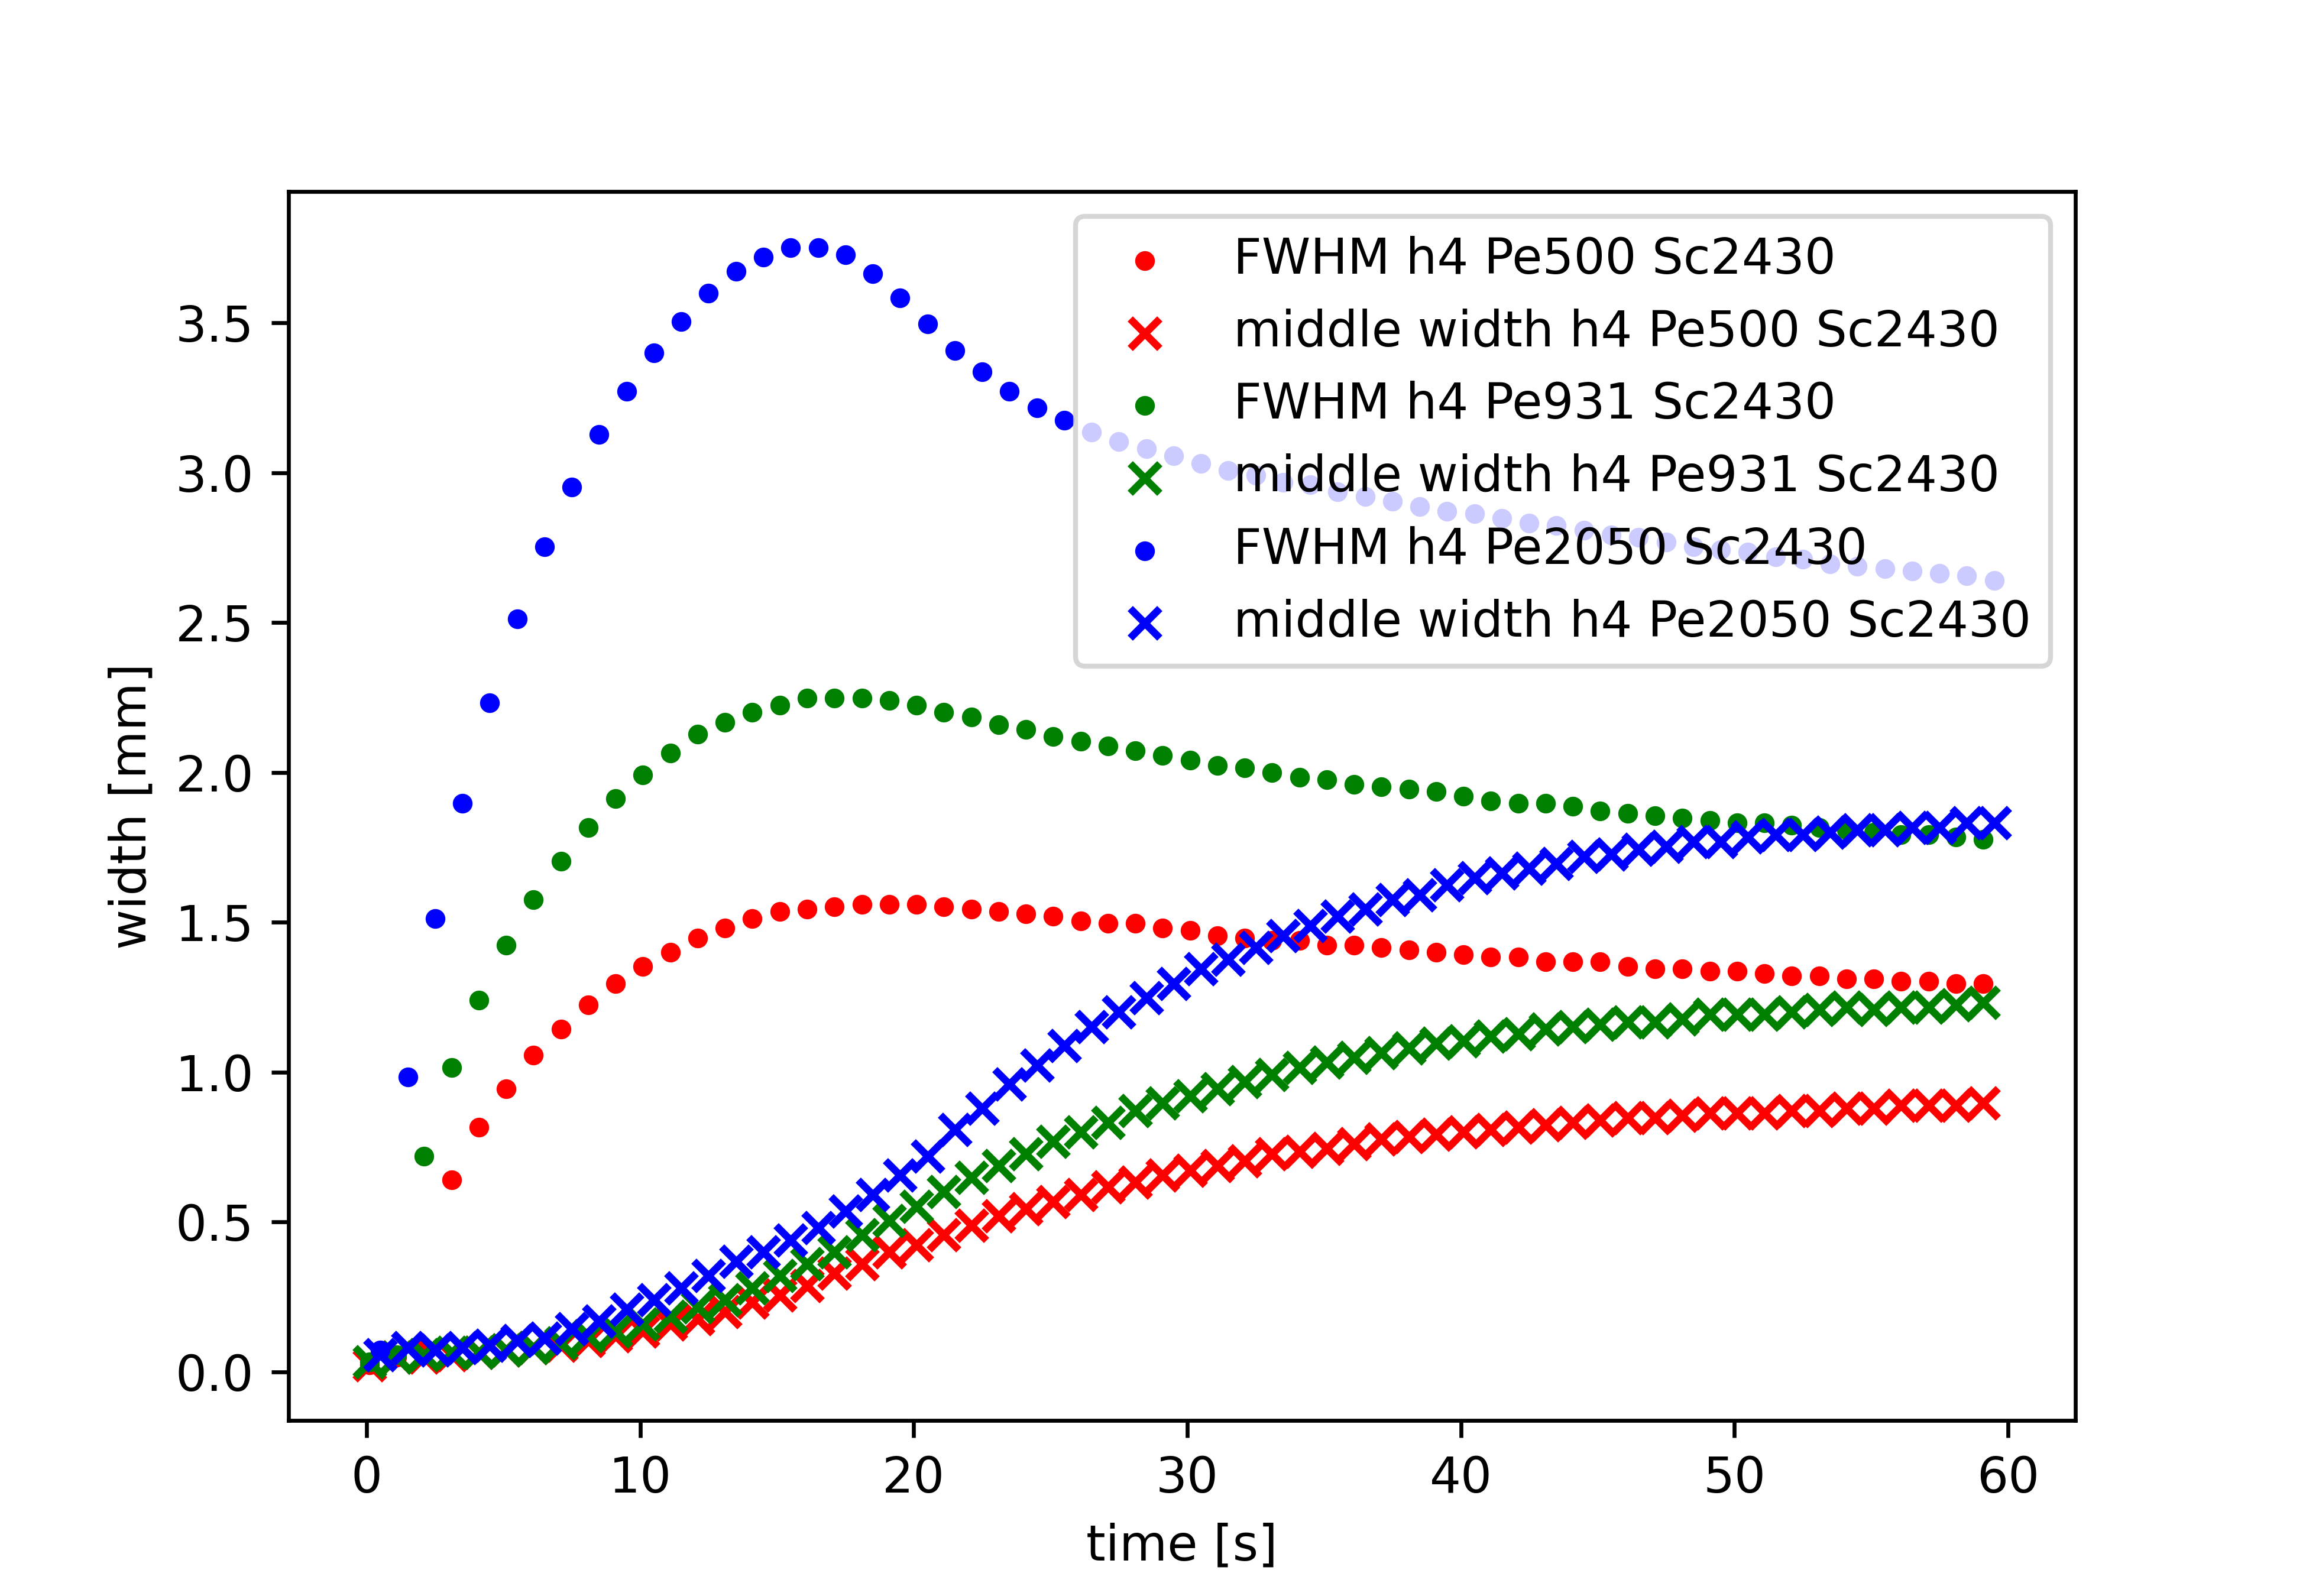
\includegraphics[width=.85\textwidth]{front_width_h4_Sc2430}
	\caption{front widths for  h = 0.4mm Sc = 2430
		\label{fig: front_width_pos_h4_Sc2430}}
\end{figure}

The cases with the lower Schmidt number does show comparable behaviour to the one for the height of 0.2mm, that do have the same Schmidt number. The FWHM curves show peaks as well but they are not that sharp and narrow compared against the ones in \autoref{fig: front_width_pos_h2_Sc2430}. The FWHMHGH behaves similar to the one with the same conditions at 0.2mm gap height, but the phase of growth is way longer and the constant value is reached near the end ot the 60 second simulation run time.

For square root like behaviour of the higher Schmidt number case can be explained by the fact that front is still in the phase of growing. This is comparable to the 0.2mm gap height cases for a time range of up to 20 seconds. For later times the FWHM is expected to decay as well as can be seen in the 0.2mm cases. The sudden growth is even more clearly visible for the gap height of 0.6mm and therefore explained there. The low growth rate of the FWHMHGH is the result of the high local Peclet number during most of the part of the simulation. The diffusive part only starts affecting this width at later times where the advective part loses it's influence on the front.

For the cases with the Schmidt number of 2430 the FWHM seems to reach its highest value in this case when the initial two different peaks visible within the concentration plots merge into one, which can be seen in \autoref{fig: pos_h4_peak_plots}. Up to a time of around 18 seconds two peaks can be distinguished within the product concentration plots. These two peaks are visible within the concentration plots, because the local Peclet number has lower values in the areas close to the walls. As a result of that, diffusion becomes more dominant in these regions even at early times. This is clearly visible when looking at the product's concentration field at a times of 2 and 10 seconds in \autoref{fig: pos_h4_peak_fields}.

\begin{figure}[htbp]
	\centering
	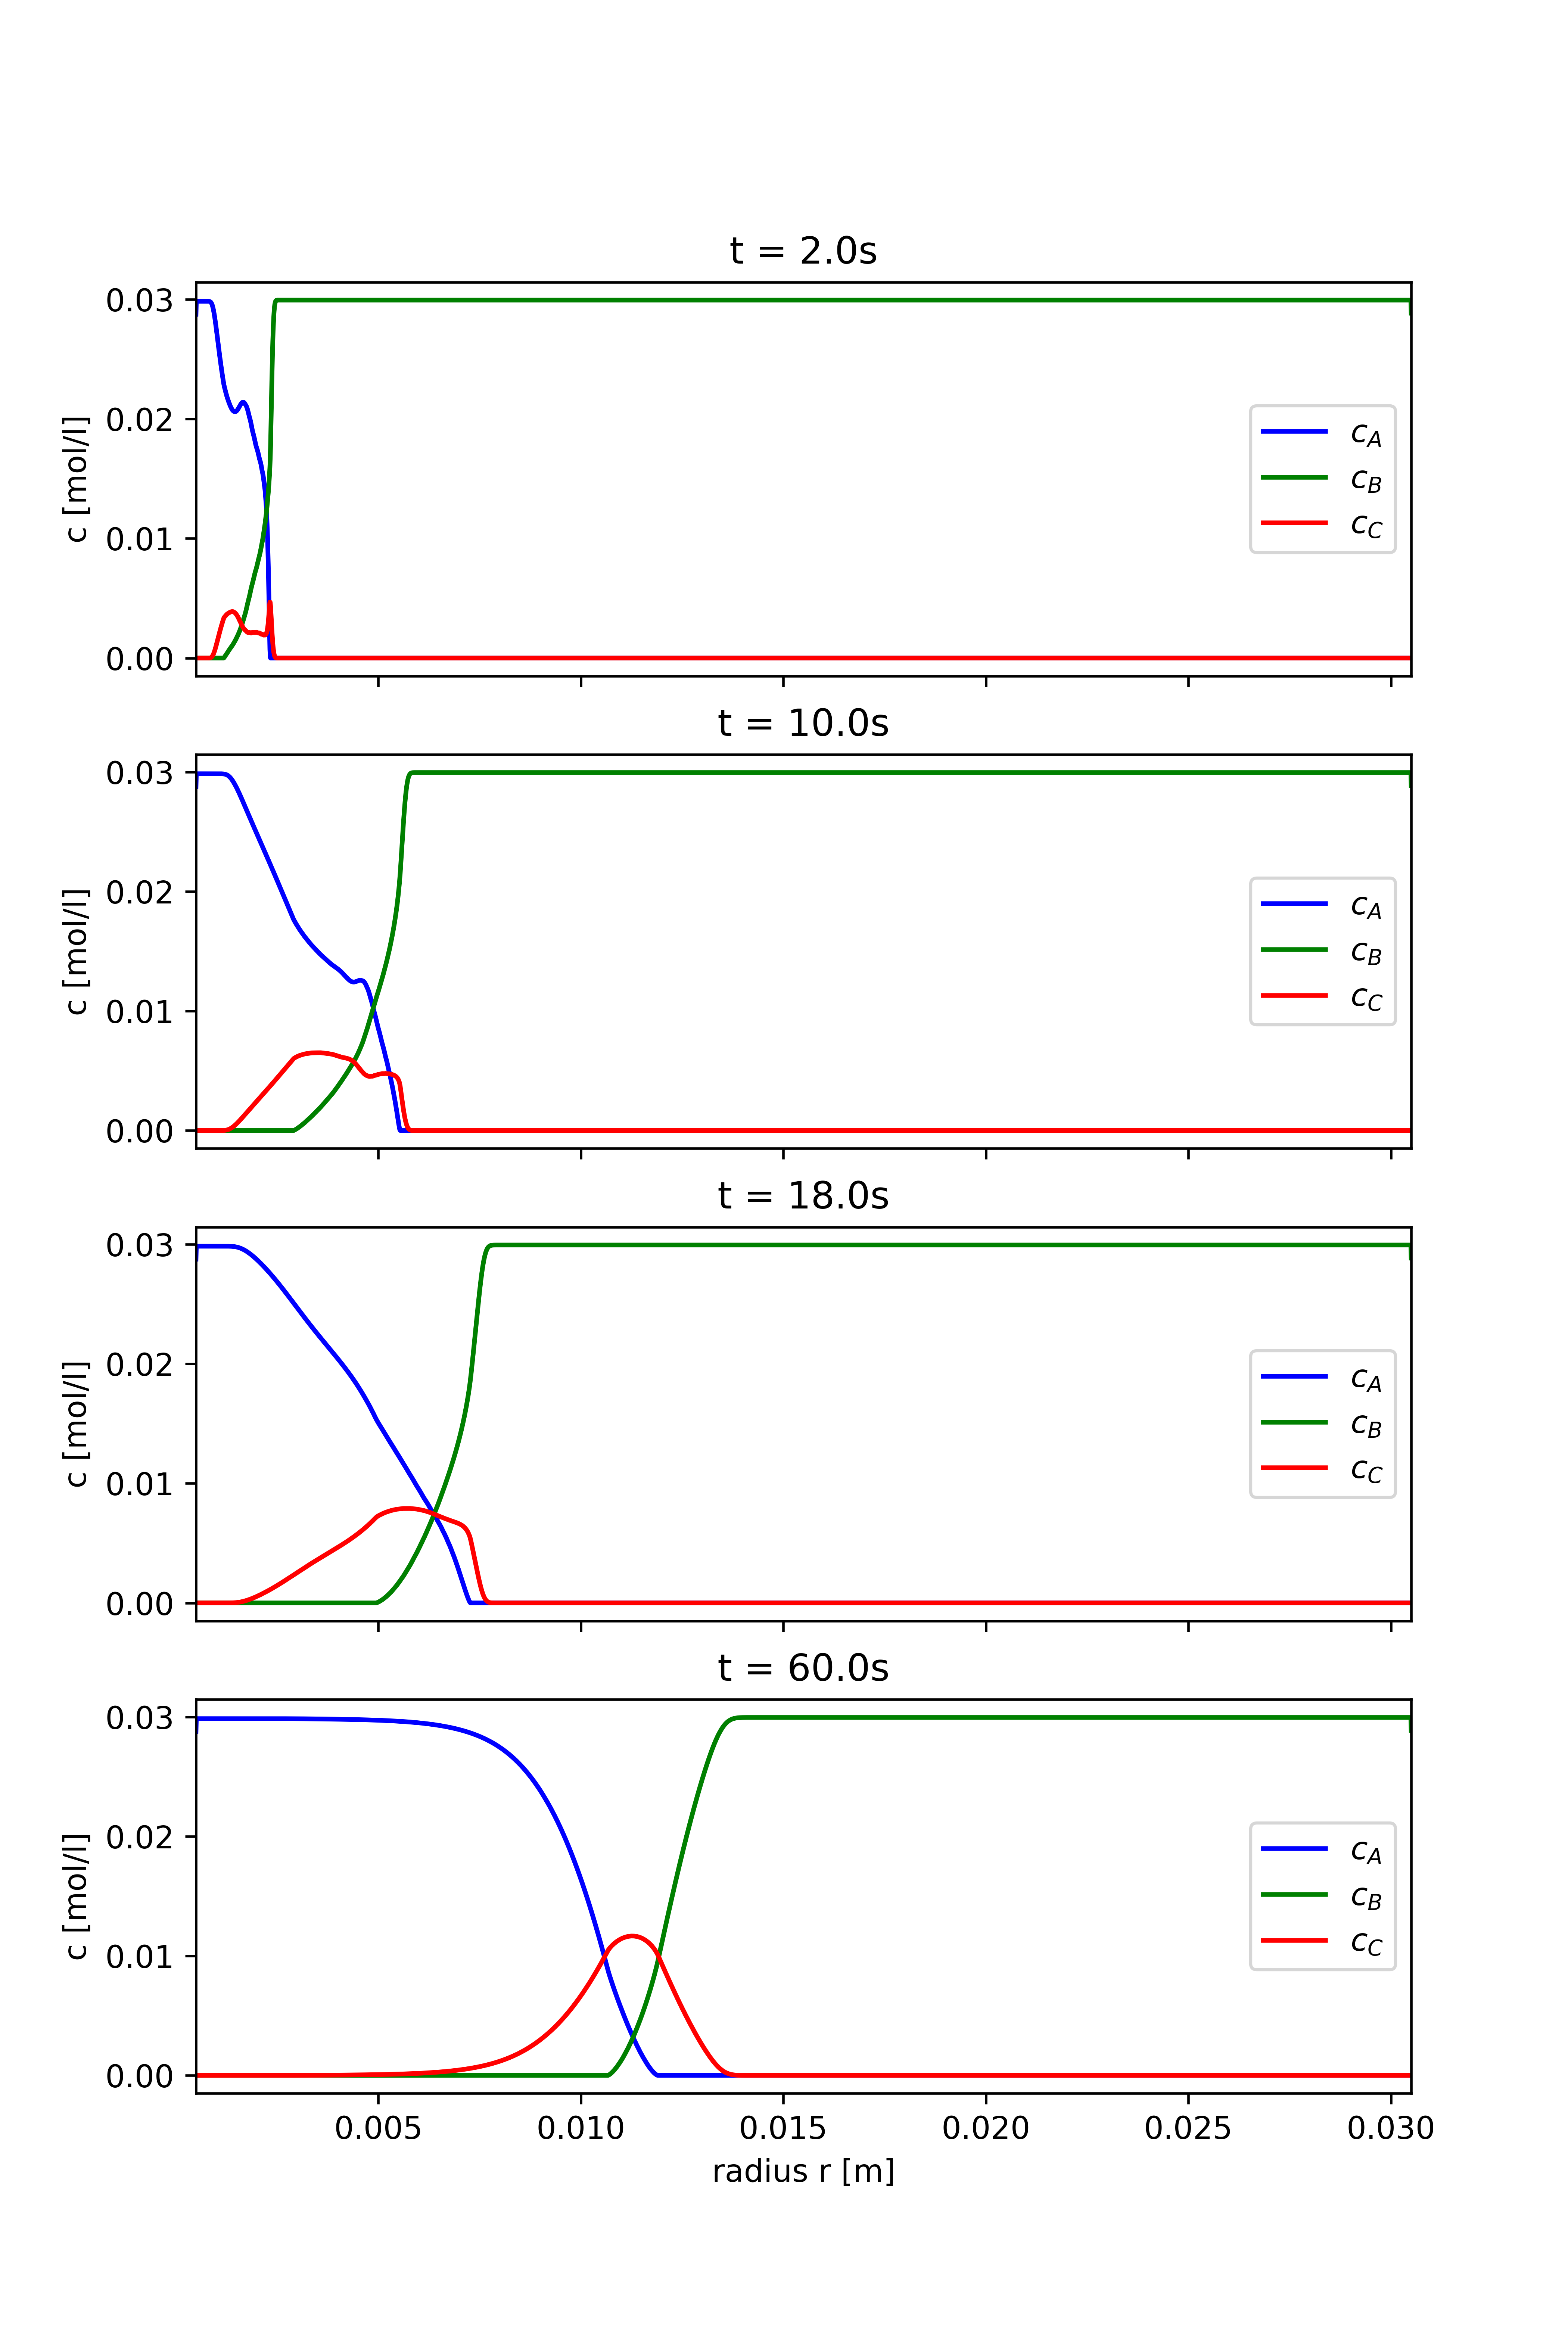
\includegraphics[width=.9\textwidth]{plot_h4r3_P205E3_S243E3_concentration-fluid_a_concentration-fluid_b_concentration-fluid_c}
	\caption{Plots for gap averaged concentrations for h = 0.4mm Pe = 2050 Sc = 2430}
	\label{fig: pos_h4_peak_plots}
\end{figure}
\begin{figure}[htbp]
	\centering
	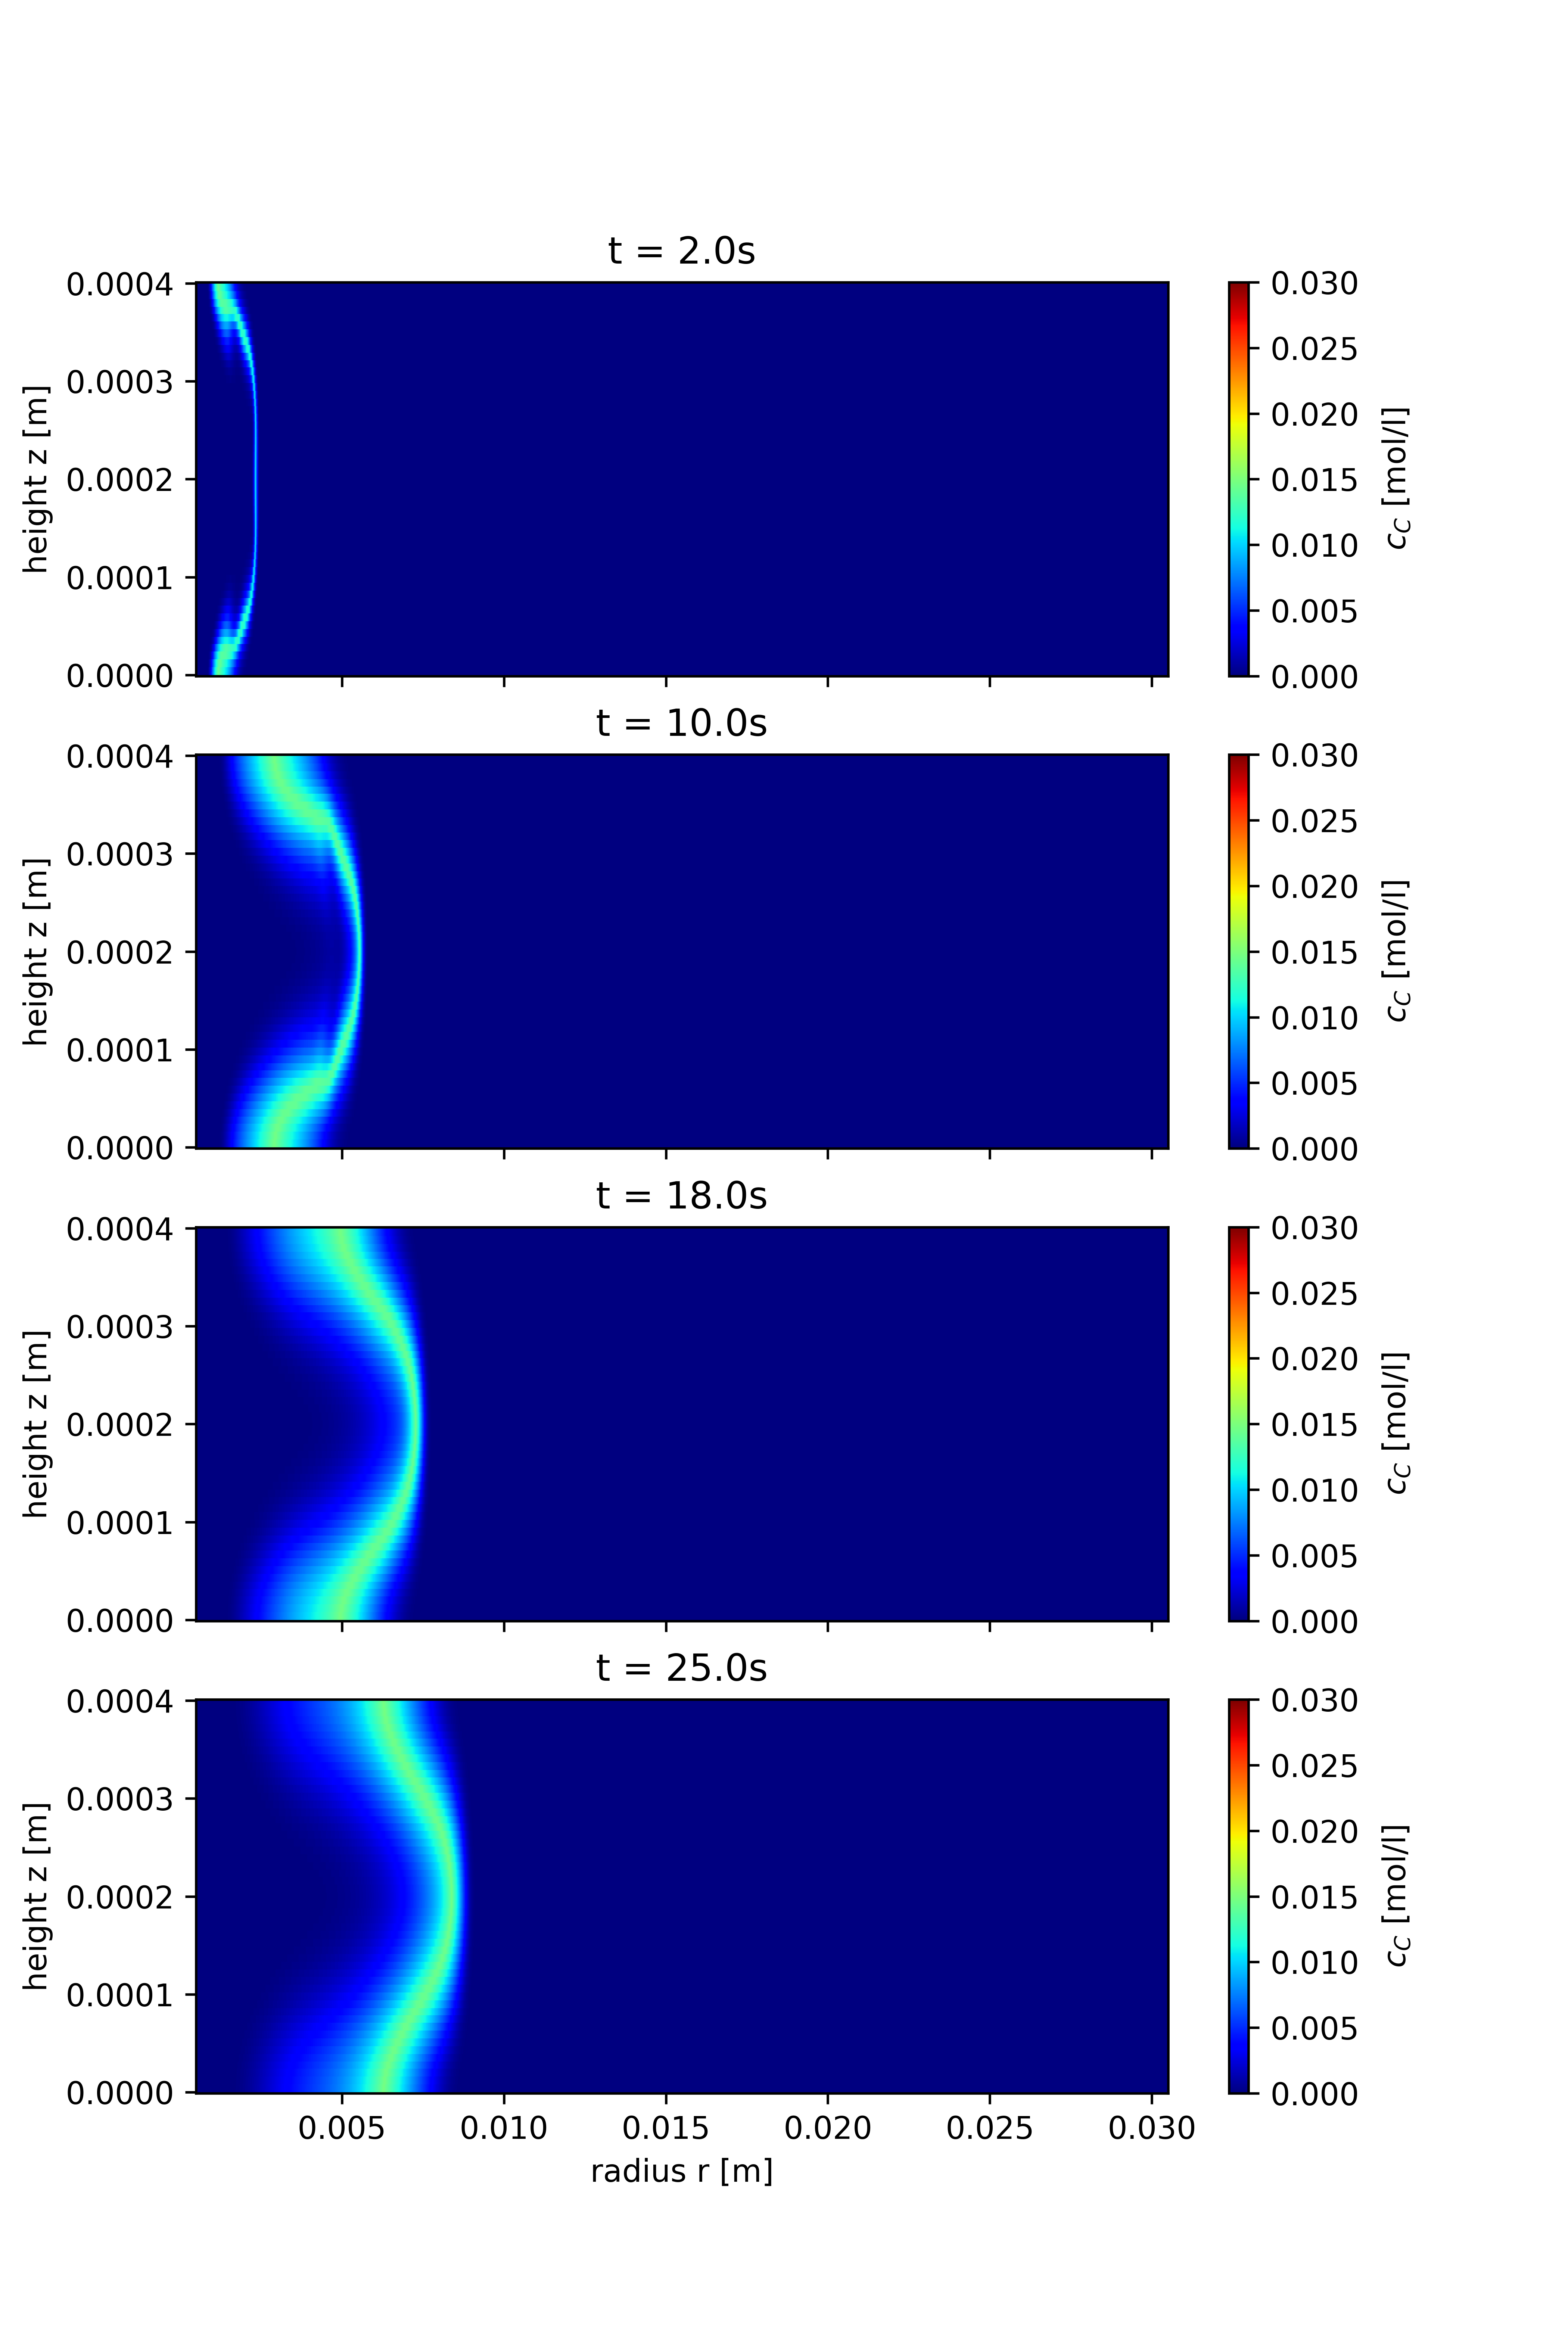
\includegraphics[width=.9\textwidth]{field_h4r3_P205E3_S243E3_concentration-fluid_c}
	\caption{Field for product concentration for h = 0.4mm Pe = 2050 Sc = 2430}
	\label{fig: pos_h4_peak_fields}
\end{figure}

At that time the front shape has reached it's maximum distortion. Within the gap averaged plot it can be seen that there is a sharp increase at the fronts front and a slow decline at its back. This decline lowers when comparing the plots for a time of 18 seconds with the one at 60 seconds in \autoref{fig: pos_h4_peak_fields}.

The FWHMHGH behaviour can be explained using the local Peclet number. At early times the front is near the inlet where the values are high so the influence of diffusion, which is the main mechanism driving the front's growth is low. Diffusion along the radial direction is the main factor, because at half the gap height the flow does not experience any shear. Advection is mainly moving the front through the reactor. While leaving the advection influence zone the FWHMHGH starts growing more rapidly, since diffusion start more and more dominating the width's growth process. The width's growths then slows down an reaches a constant value due the fact that an equilibrium between diffusion and the reaction is reached. The differences in the FWHMHGH curves, when comparing different Schmidt numbers can be explained by different diffusion coefficients. The higher the diffusion coefficient the sooner the growth starts and the final constant value is reached.
\newline

For the case with a gap height of 0.6mm the width's behaviour seems to change quite significantly compared to the 0.4mm case. 
\begin{figure}[htb]
	\centering
	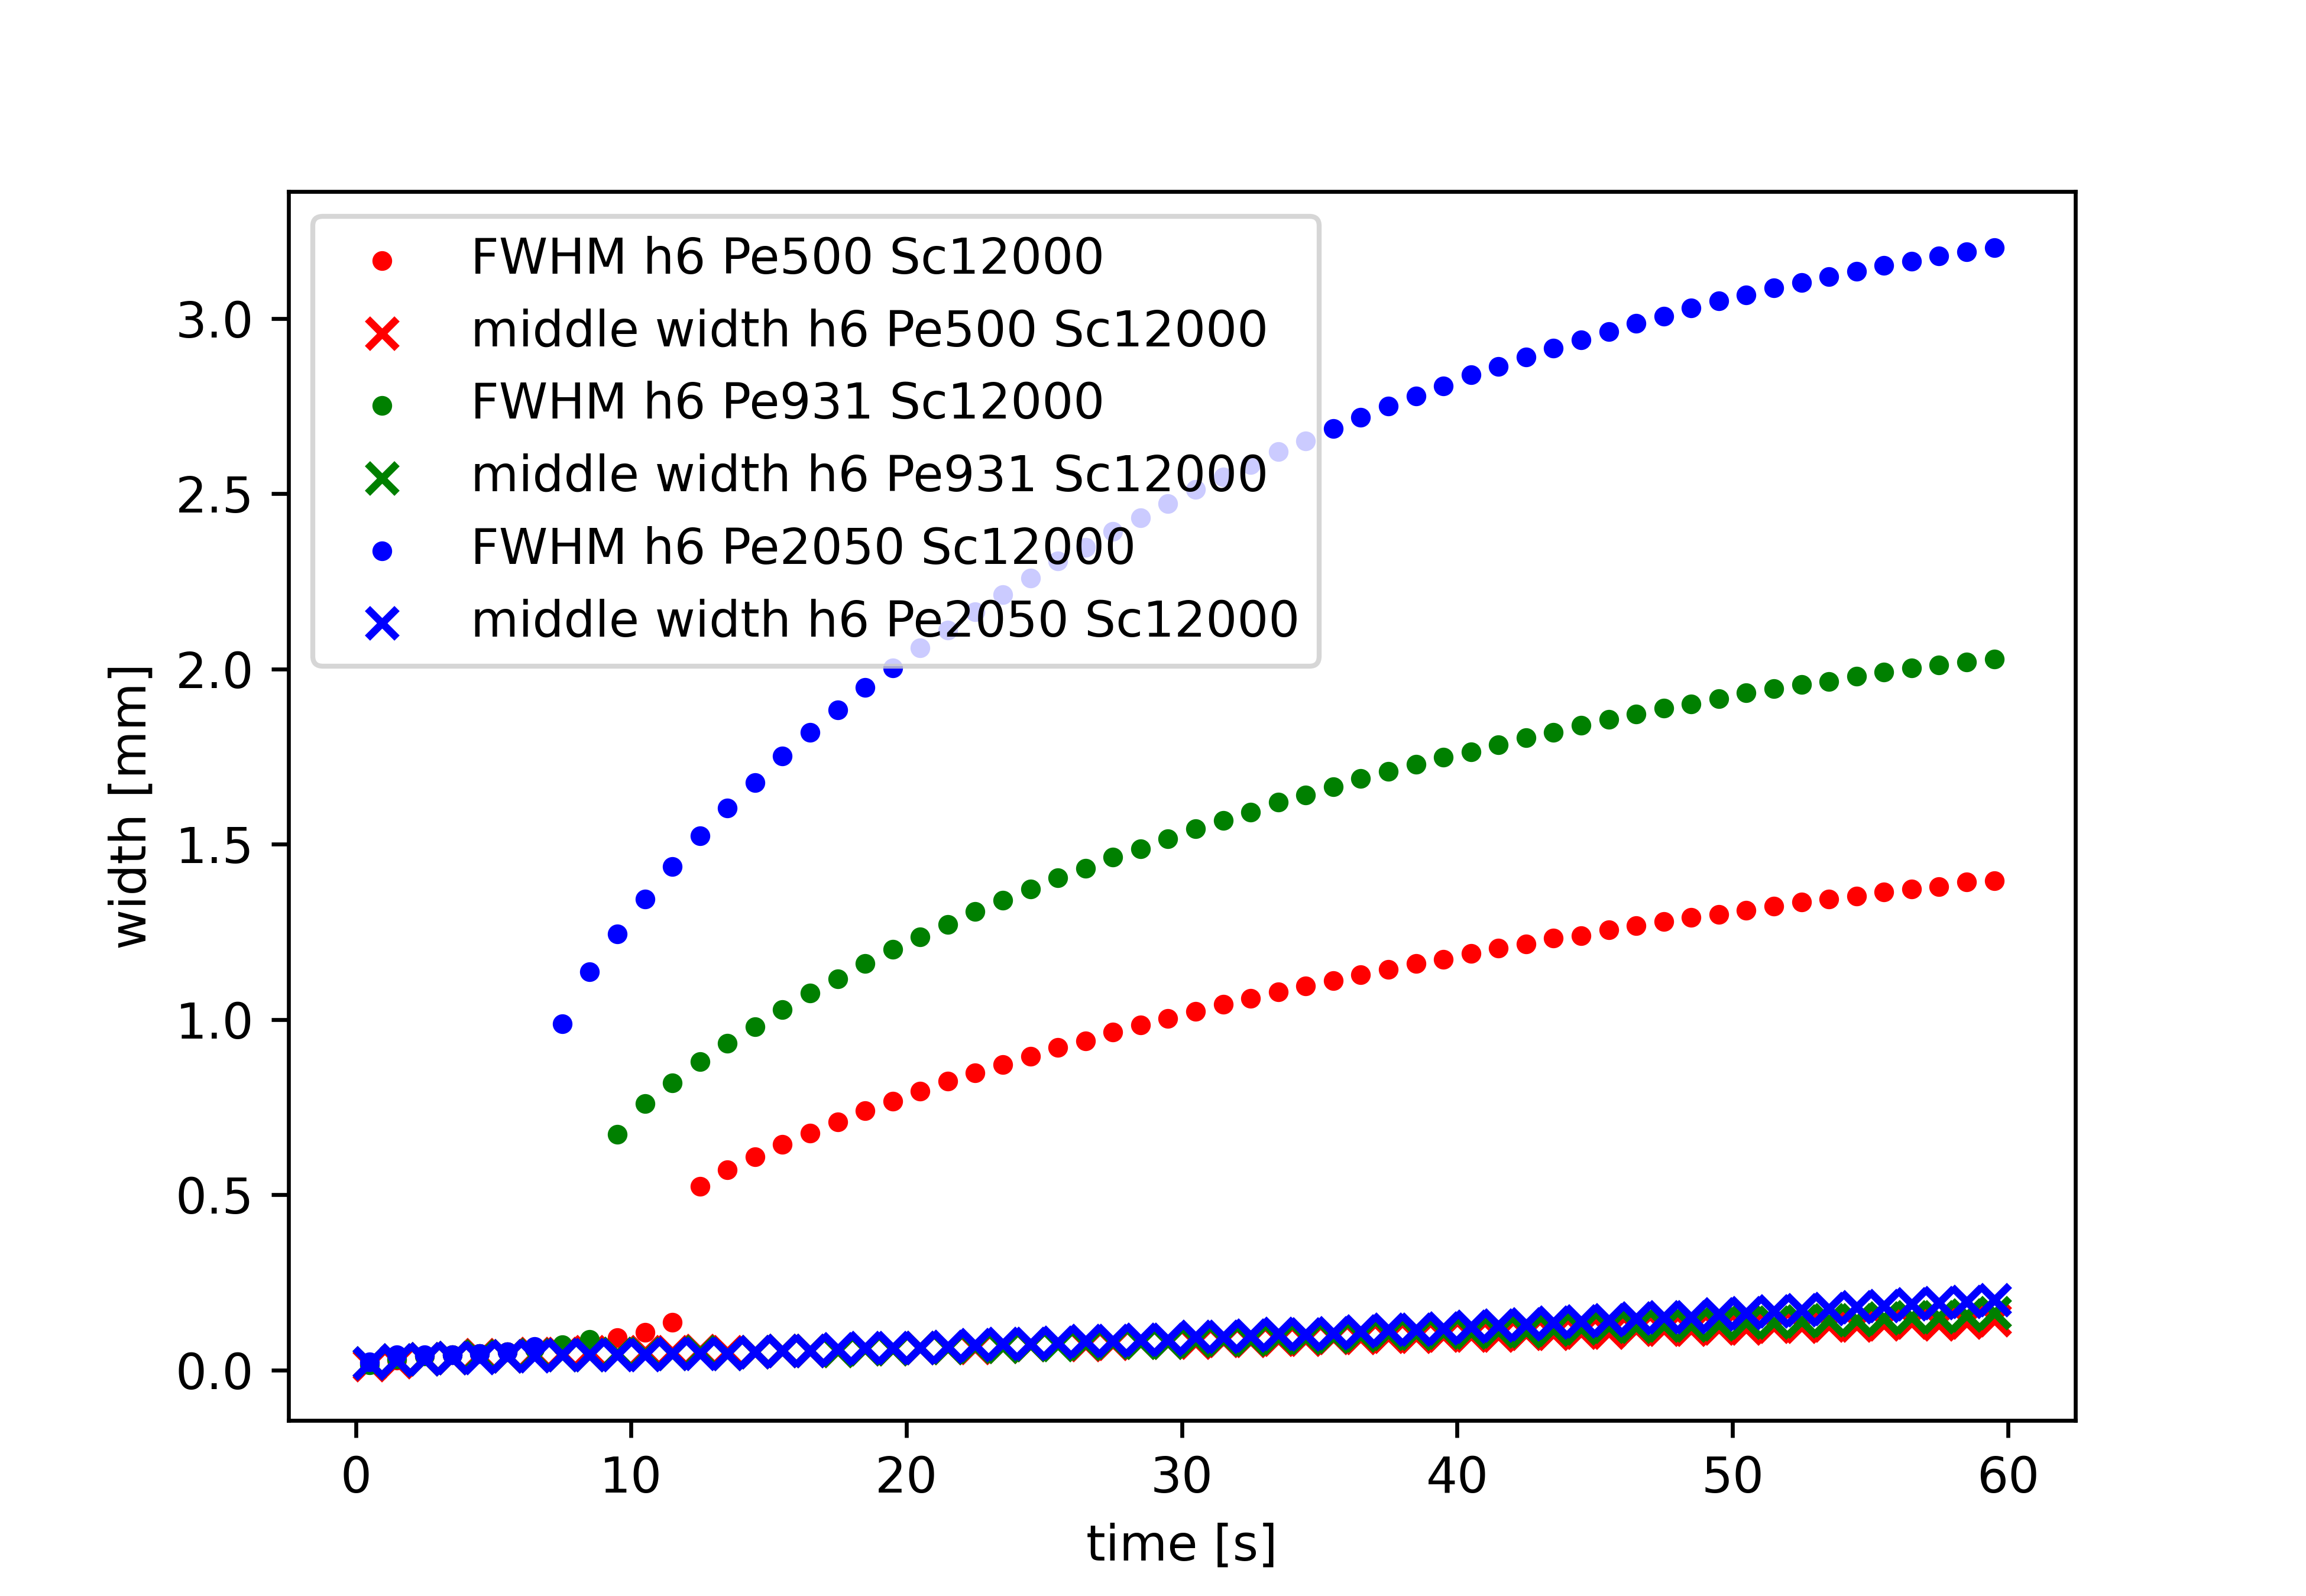
\includegraphics[width=.9\linewidth]{front_width_h6_Sc12000}
	\caption{front widths for  h = 0.6mm Sc = 12000}
	\label{fig: front_width_h6_Sc12000}
\end{figure}
For the Schmidt number of 12000 the width's results are shown in \autoref{fig: front_width_h6_Sc12000}. The general form of the FWHM curves seems to match the ones from the previous discussed cases. A difference, compared to the 0.4mm cases, is that the width's growth seems to start delayed even more at around 8 to 12 seconds. The FWHMHGH does not grow at all for this Schmidt number.
\begin{figure}[htb]
	\centering
	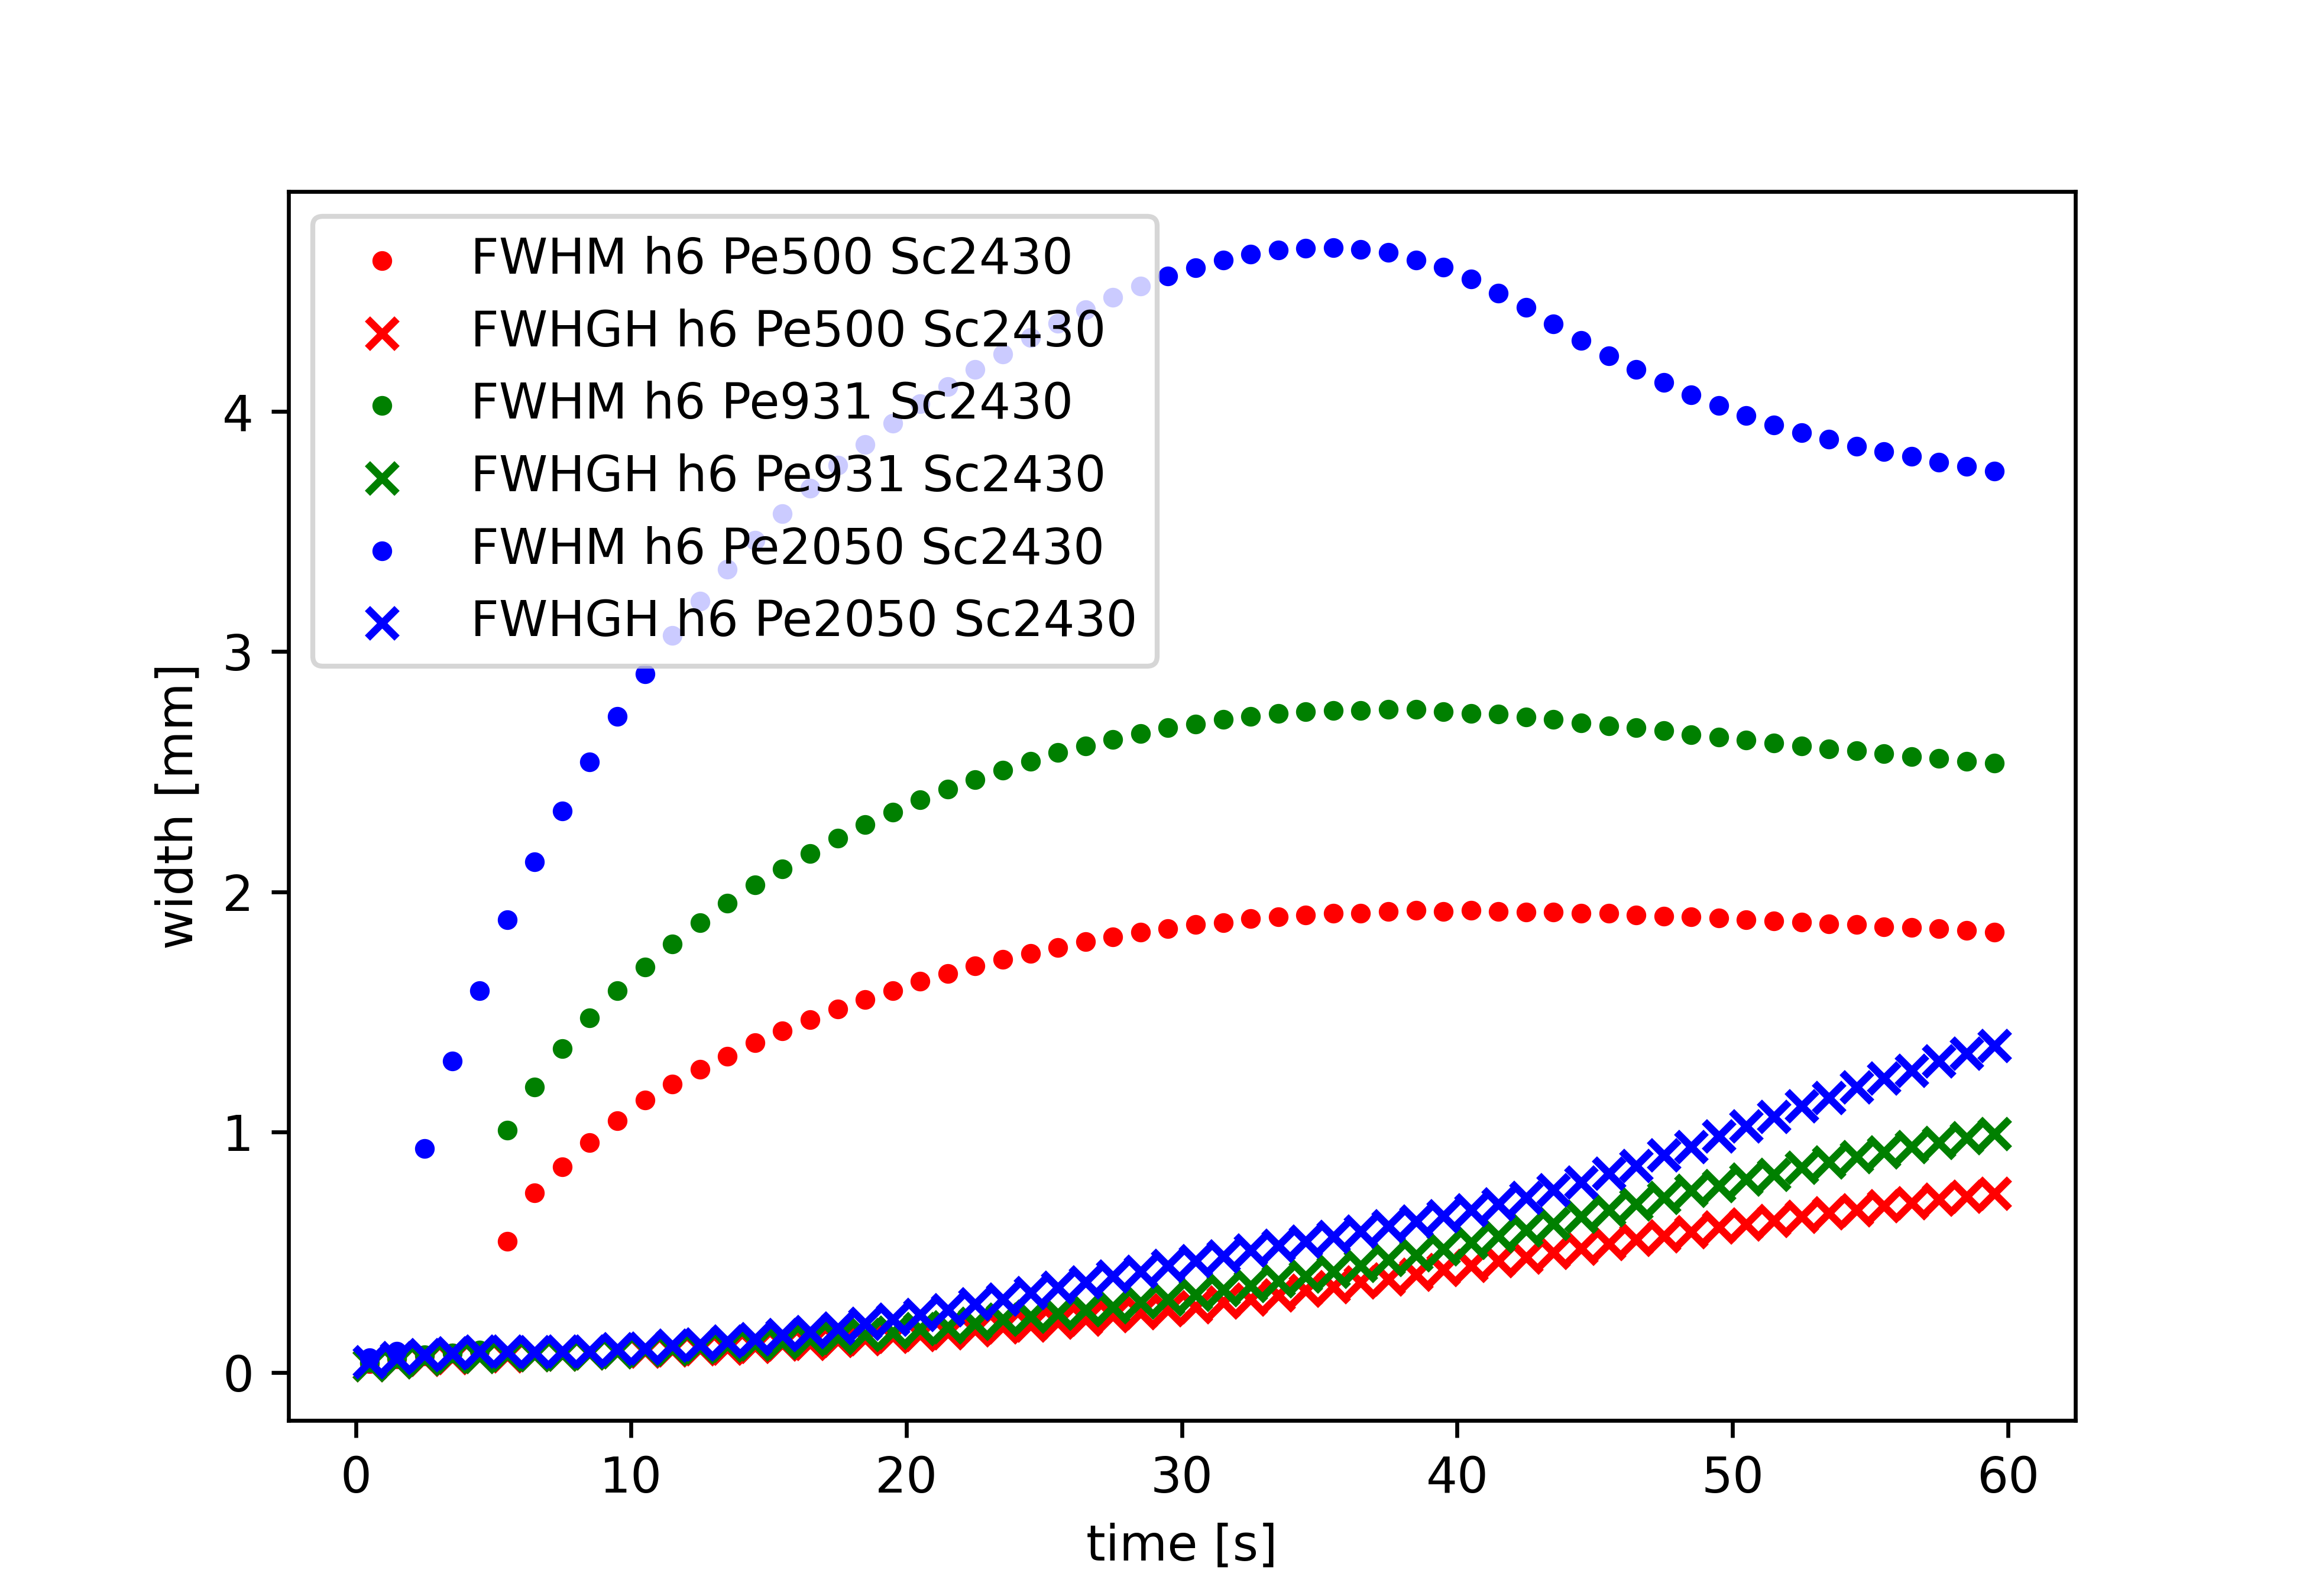
\includegraphics[width=.9\linewidth]{front_width_h6_Sc2430}
	\caption{front widths for  h = 0.6mm Sc = 2430}
	\label{fig: front_width_pos_h6_Sc2430}
\end{figure}
I am here now.

A slight delay can also be seen within the 0.4mm case. Within \autoref{fig: plots_early} the concentration plots are shown for the gap height of 0.4mm and 0.6mm for a Peclet number of 931 and a Schmidt number of 12000 close to the inlet. Within these two plots it can seen that the initial spike in the front start decaying over time. The moment the value of $0.5 \cdot c_{c,max}$ falls into the region above 0 and below the value at the back of the front the front's width suddenly jumps to a higher value.
\begin{figure}[htb]
	\centering
	\subfloat[\centering  h = 0.6mm case]{{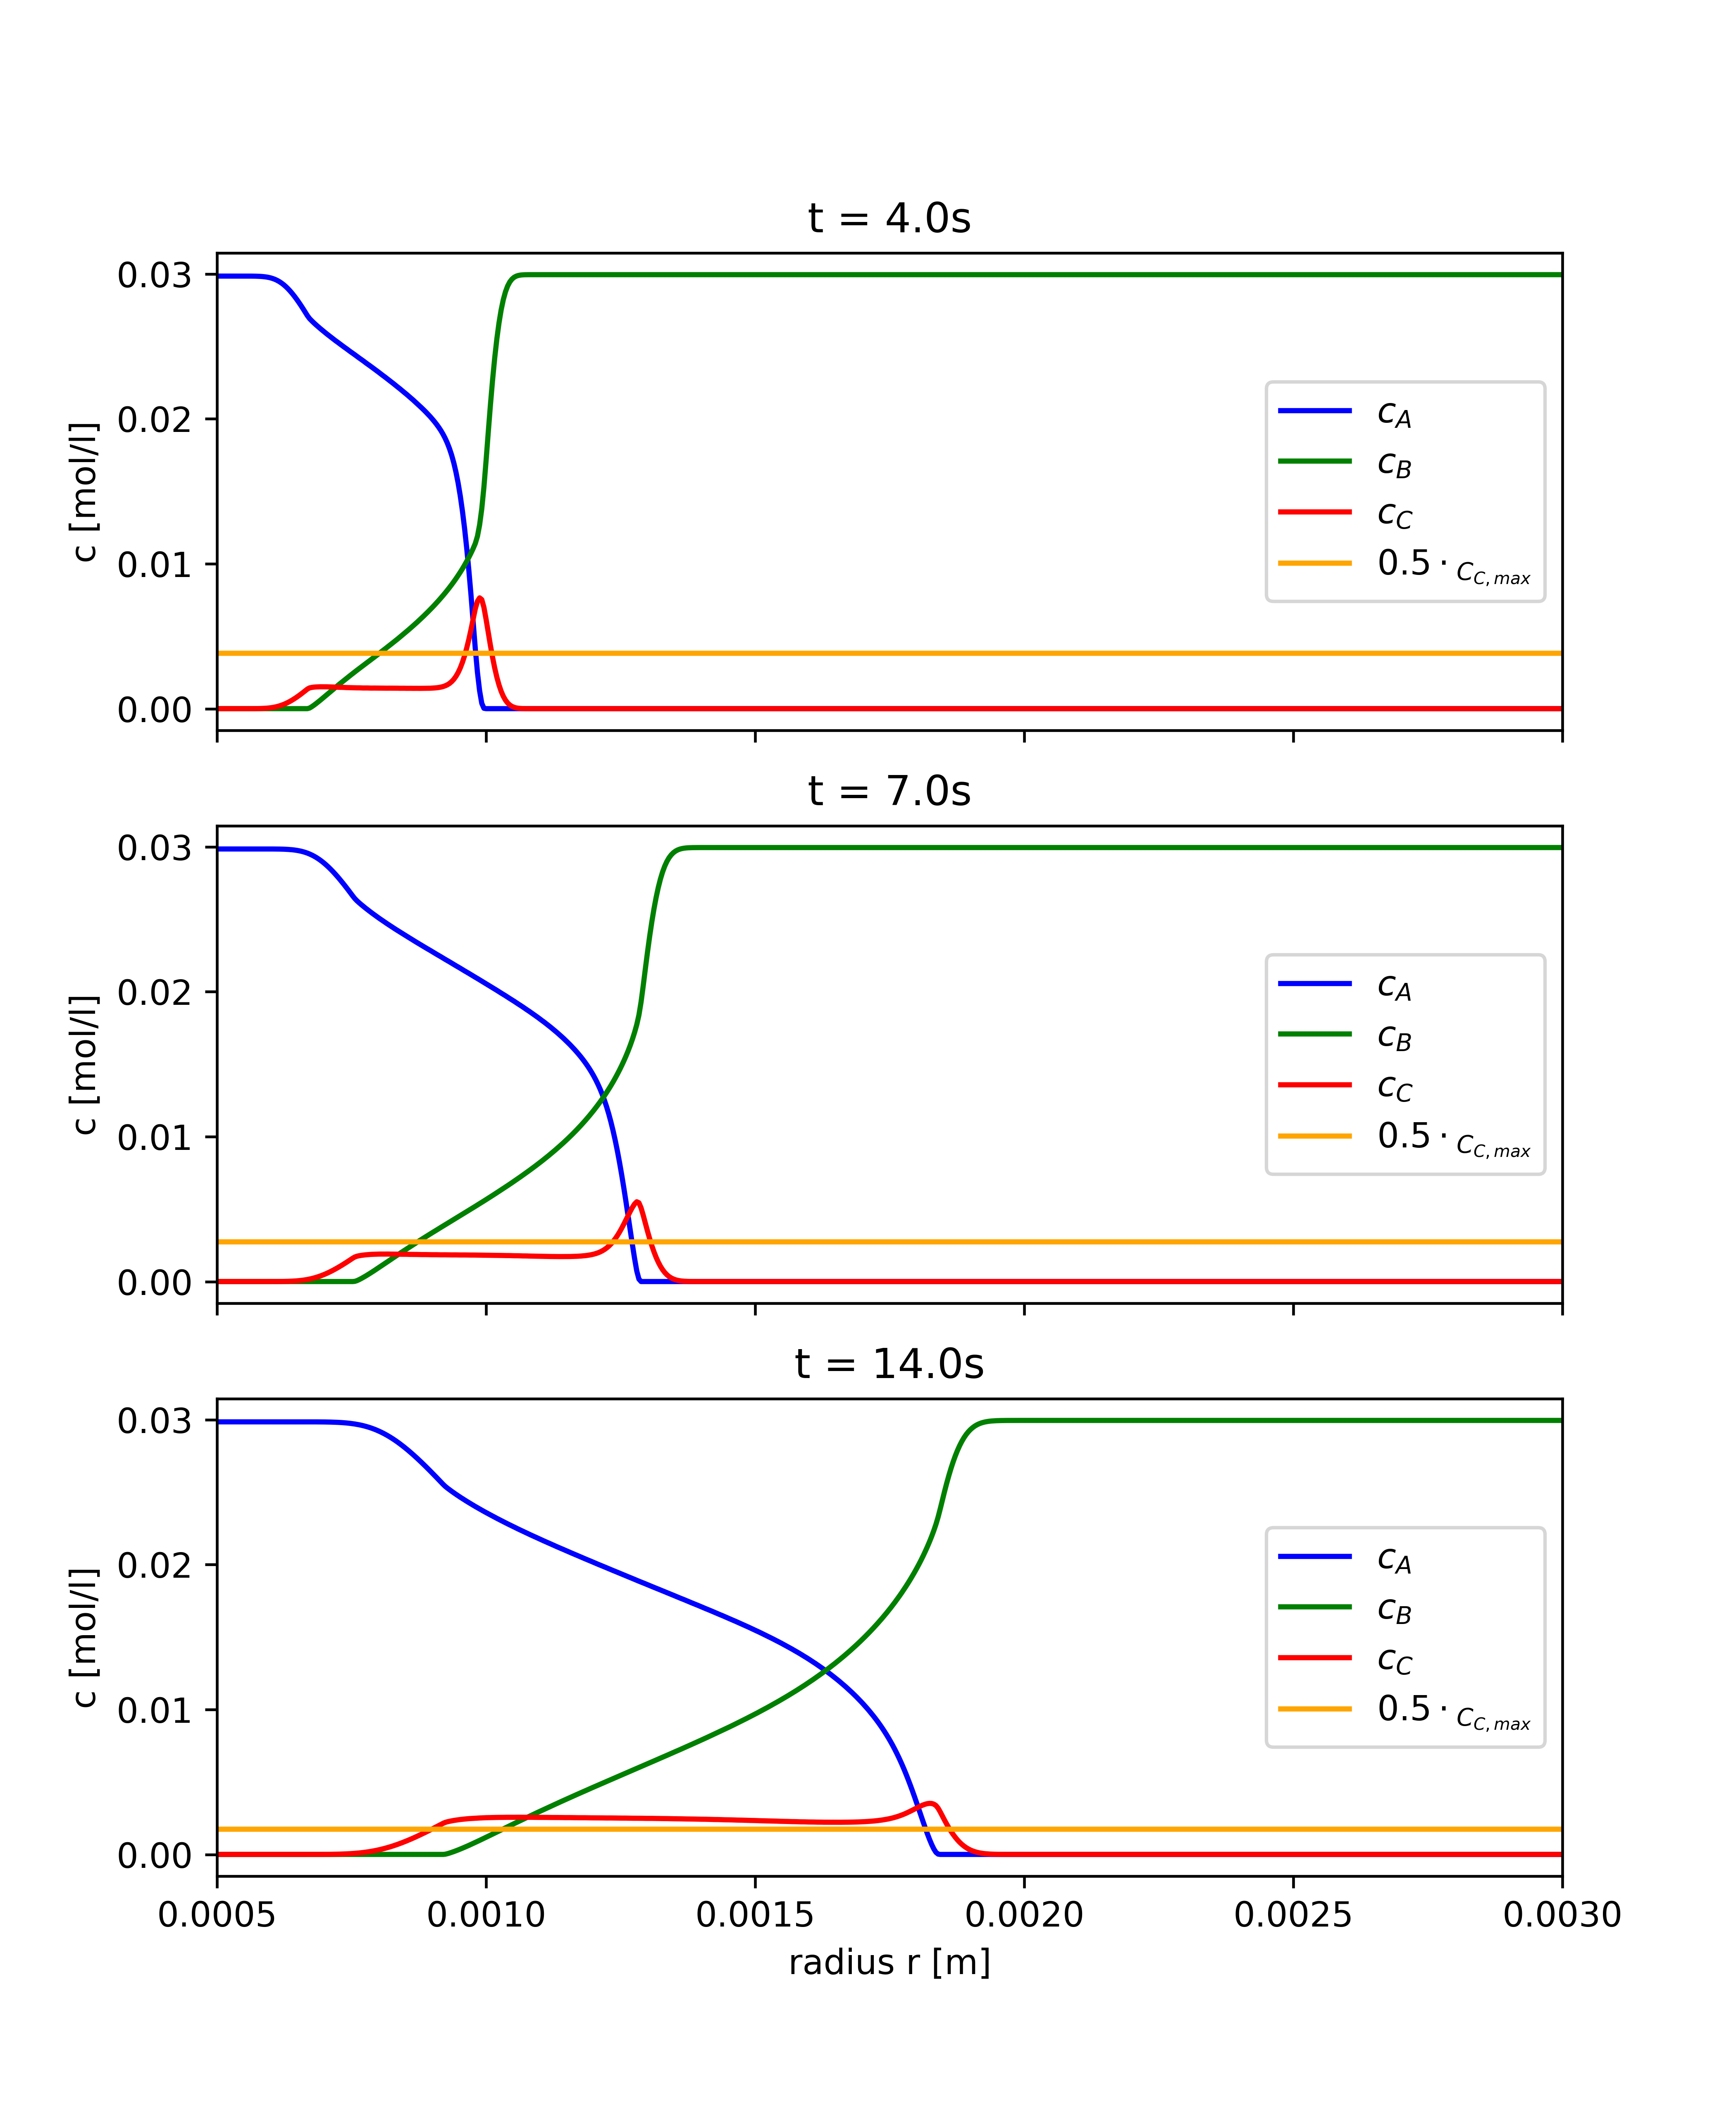
\includegraphics[angle=0, scale=0.41]{plot_h6r3_P931E2_S120E4_concentration-fluid_a_concentration-fluid_b_concentration-fluid_c} }}%
	\qquad
	\subfloat[\centering  h = 0.4mm case]{{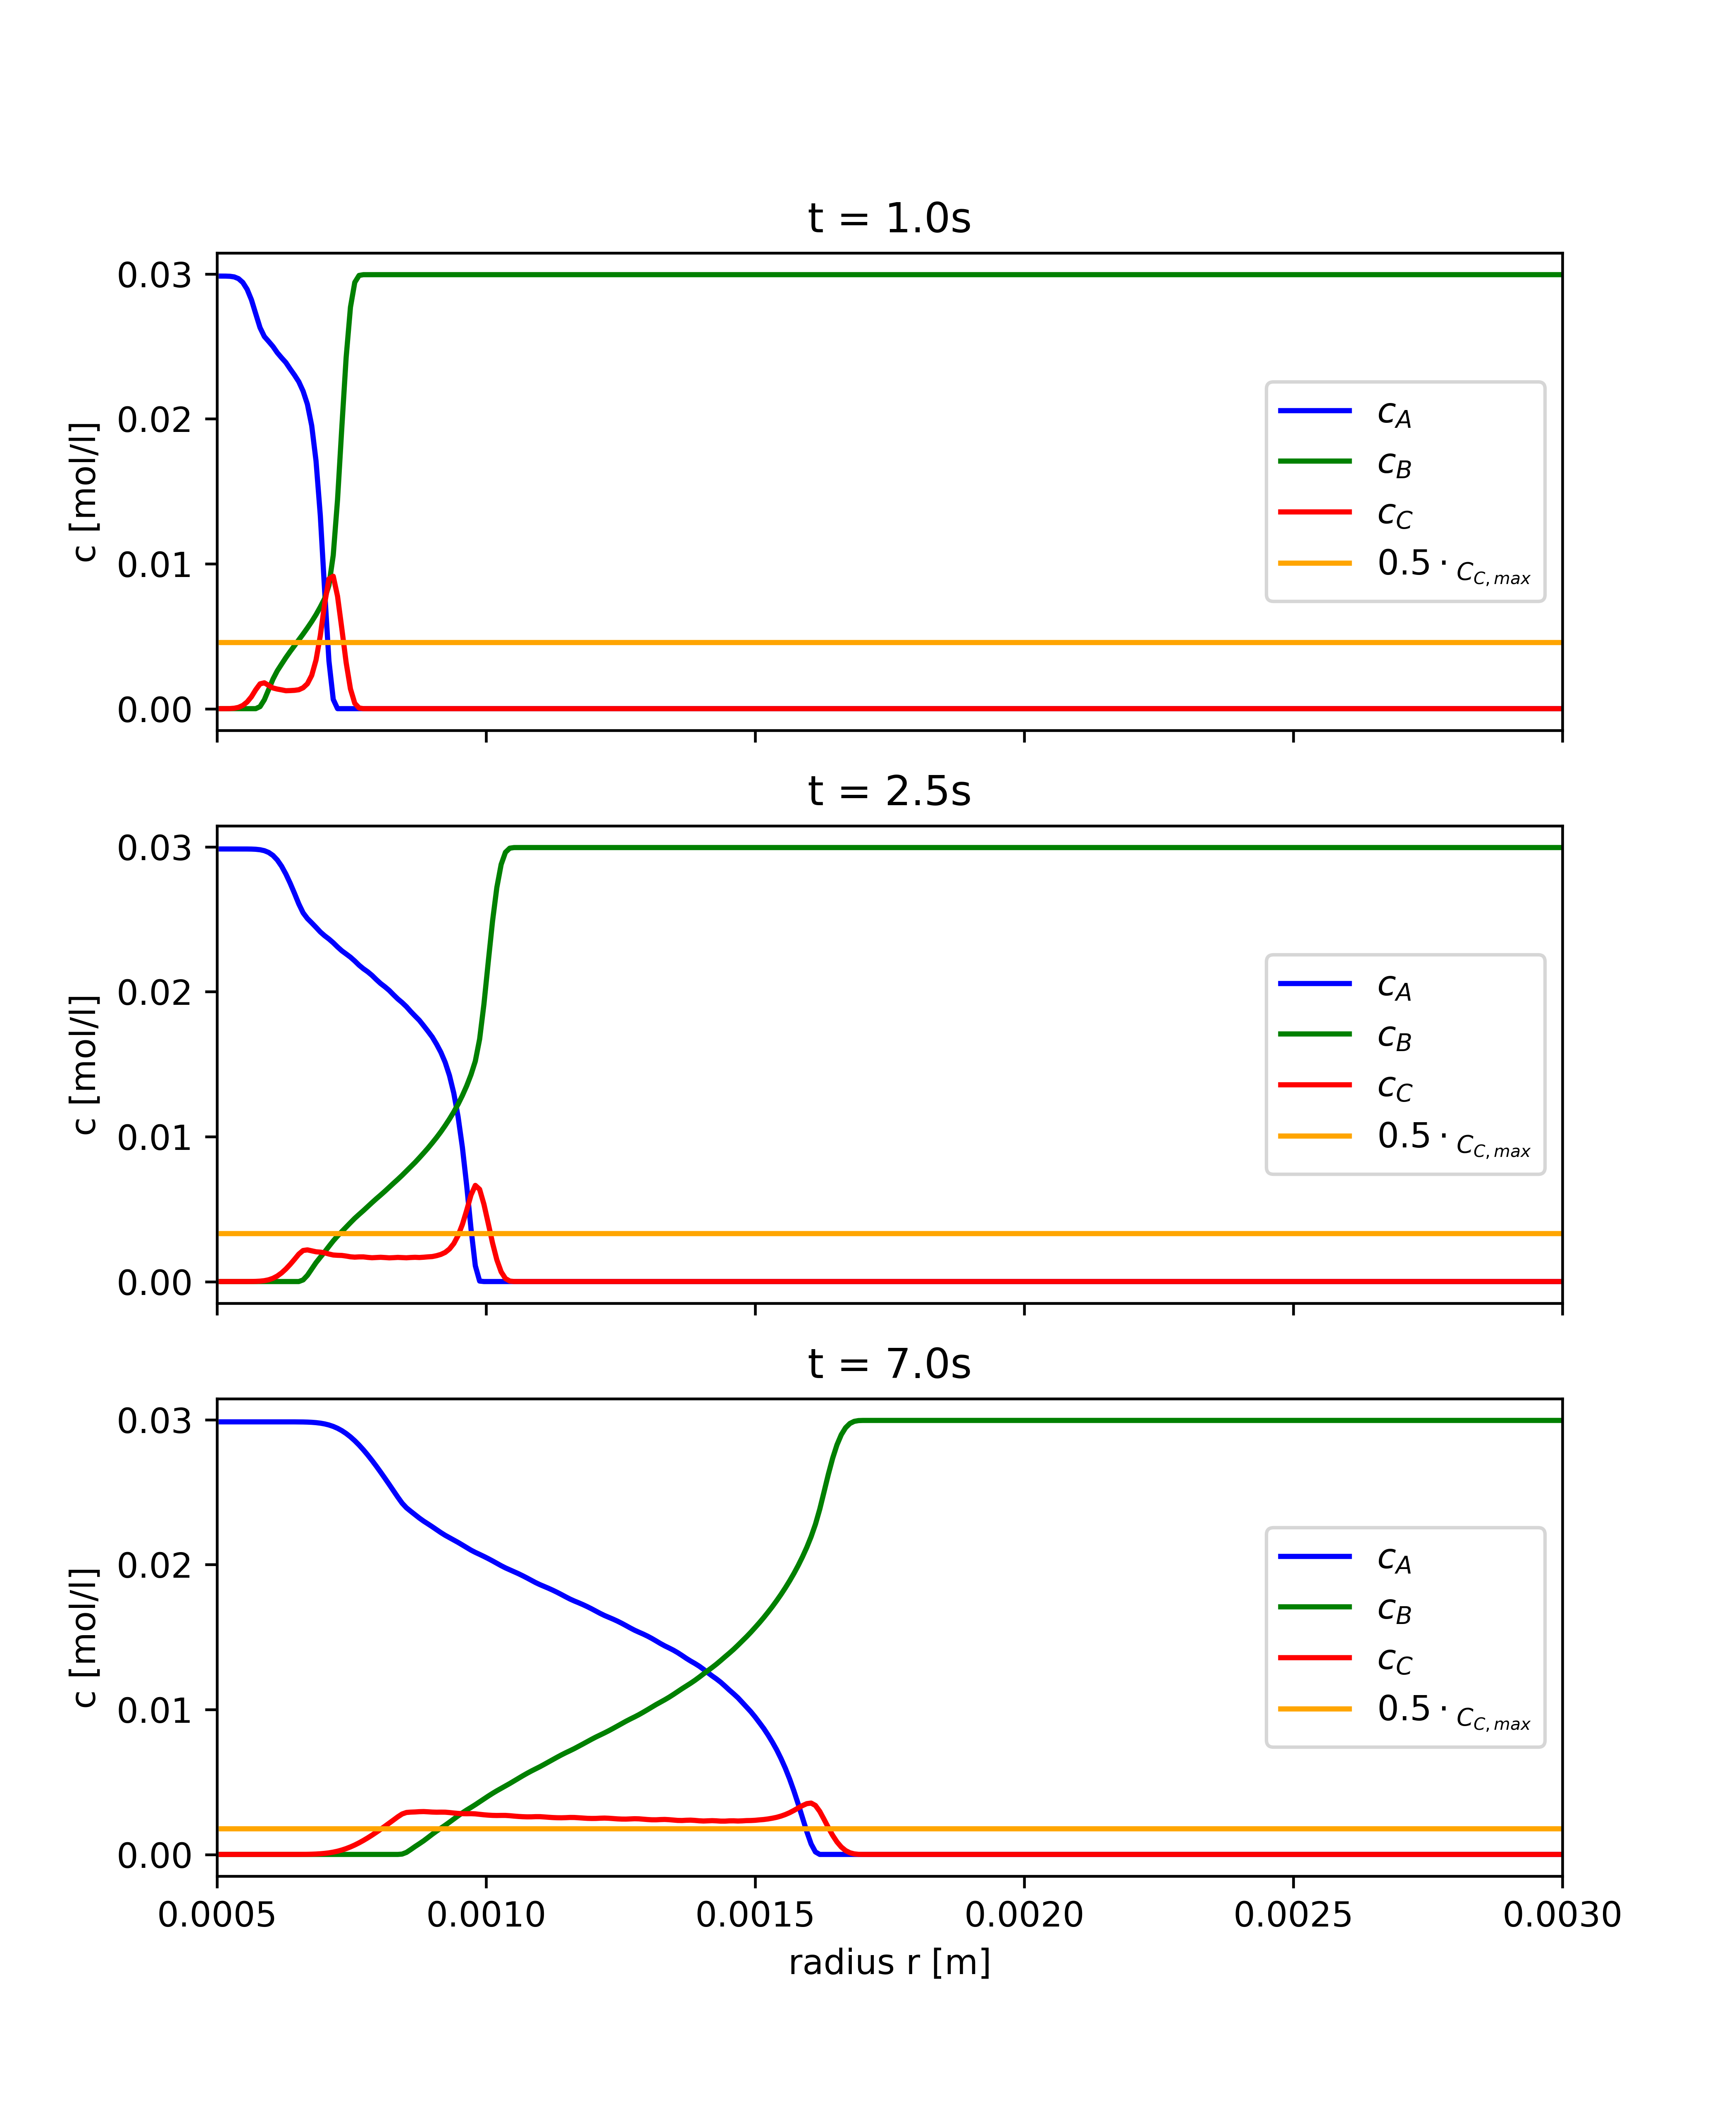
\includegraphics[angle=0, scale=0.41]{plot_h4r3_P931E2_S120E4_concentration-fluid_a_concentration-fluid_b_concentration-fluid_c copy} }}%
	\caption{concentration plots for  Pe = 931 Sc = 12000}%
	\label{fig: plots_early}%
\end{figure}
The width at the middle of the reactor only reaches very low values and doesn't grow much within the 60 seconds runtime of the simulation. When looking at the behaviour of the FWHMHGH at the lower Schmid-Number the growth seems to start at around 20 seconds and the growth accelerates slowly until the end. The FWHM in comparison reaches its peak value at times around 30 to 40 seconds for the higher Schmidt number. The growth is delayed for the FWHM width as well but not by the amount to be seen within the plot for $Sc = 12000$. The reason is the same one as explained with \autoref{fig: plots_early}.

All in all the front widths show different behaviour dependent on the conditions set for the cases. Changing the Schmidt number poses a significant change within the results as showed and discussed. The Peclet number seems to mostly influence the width's maximum peak value but doesn't change the general behaviour of the front.

\section{Formed Product}

Within this section the total product formed is investigated.

\begin{figure}[htbp]
	\centering
	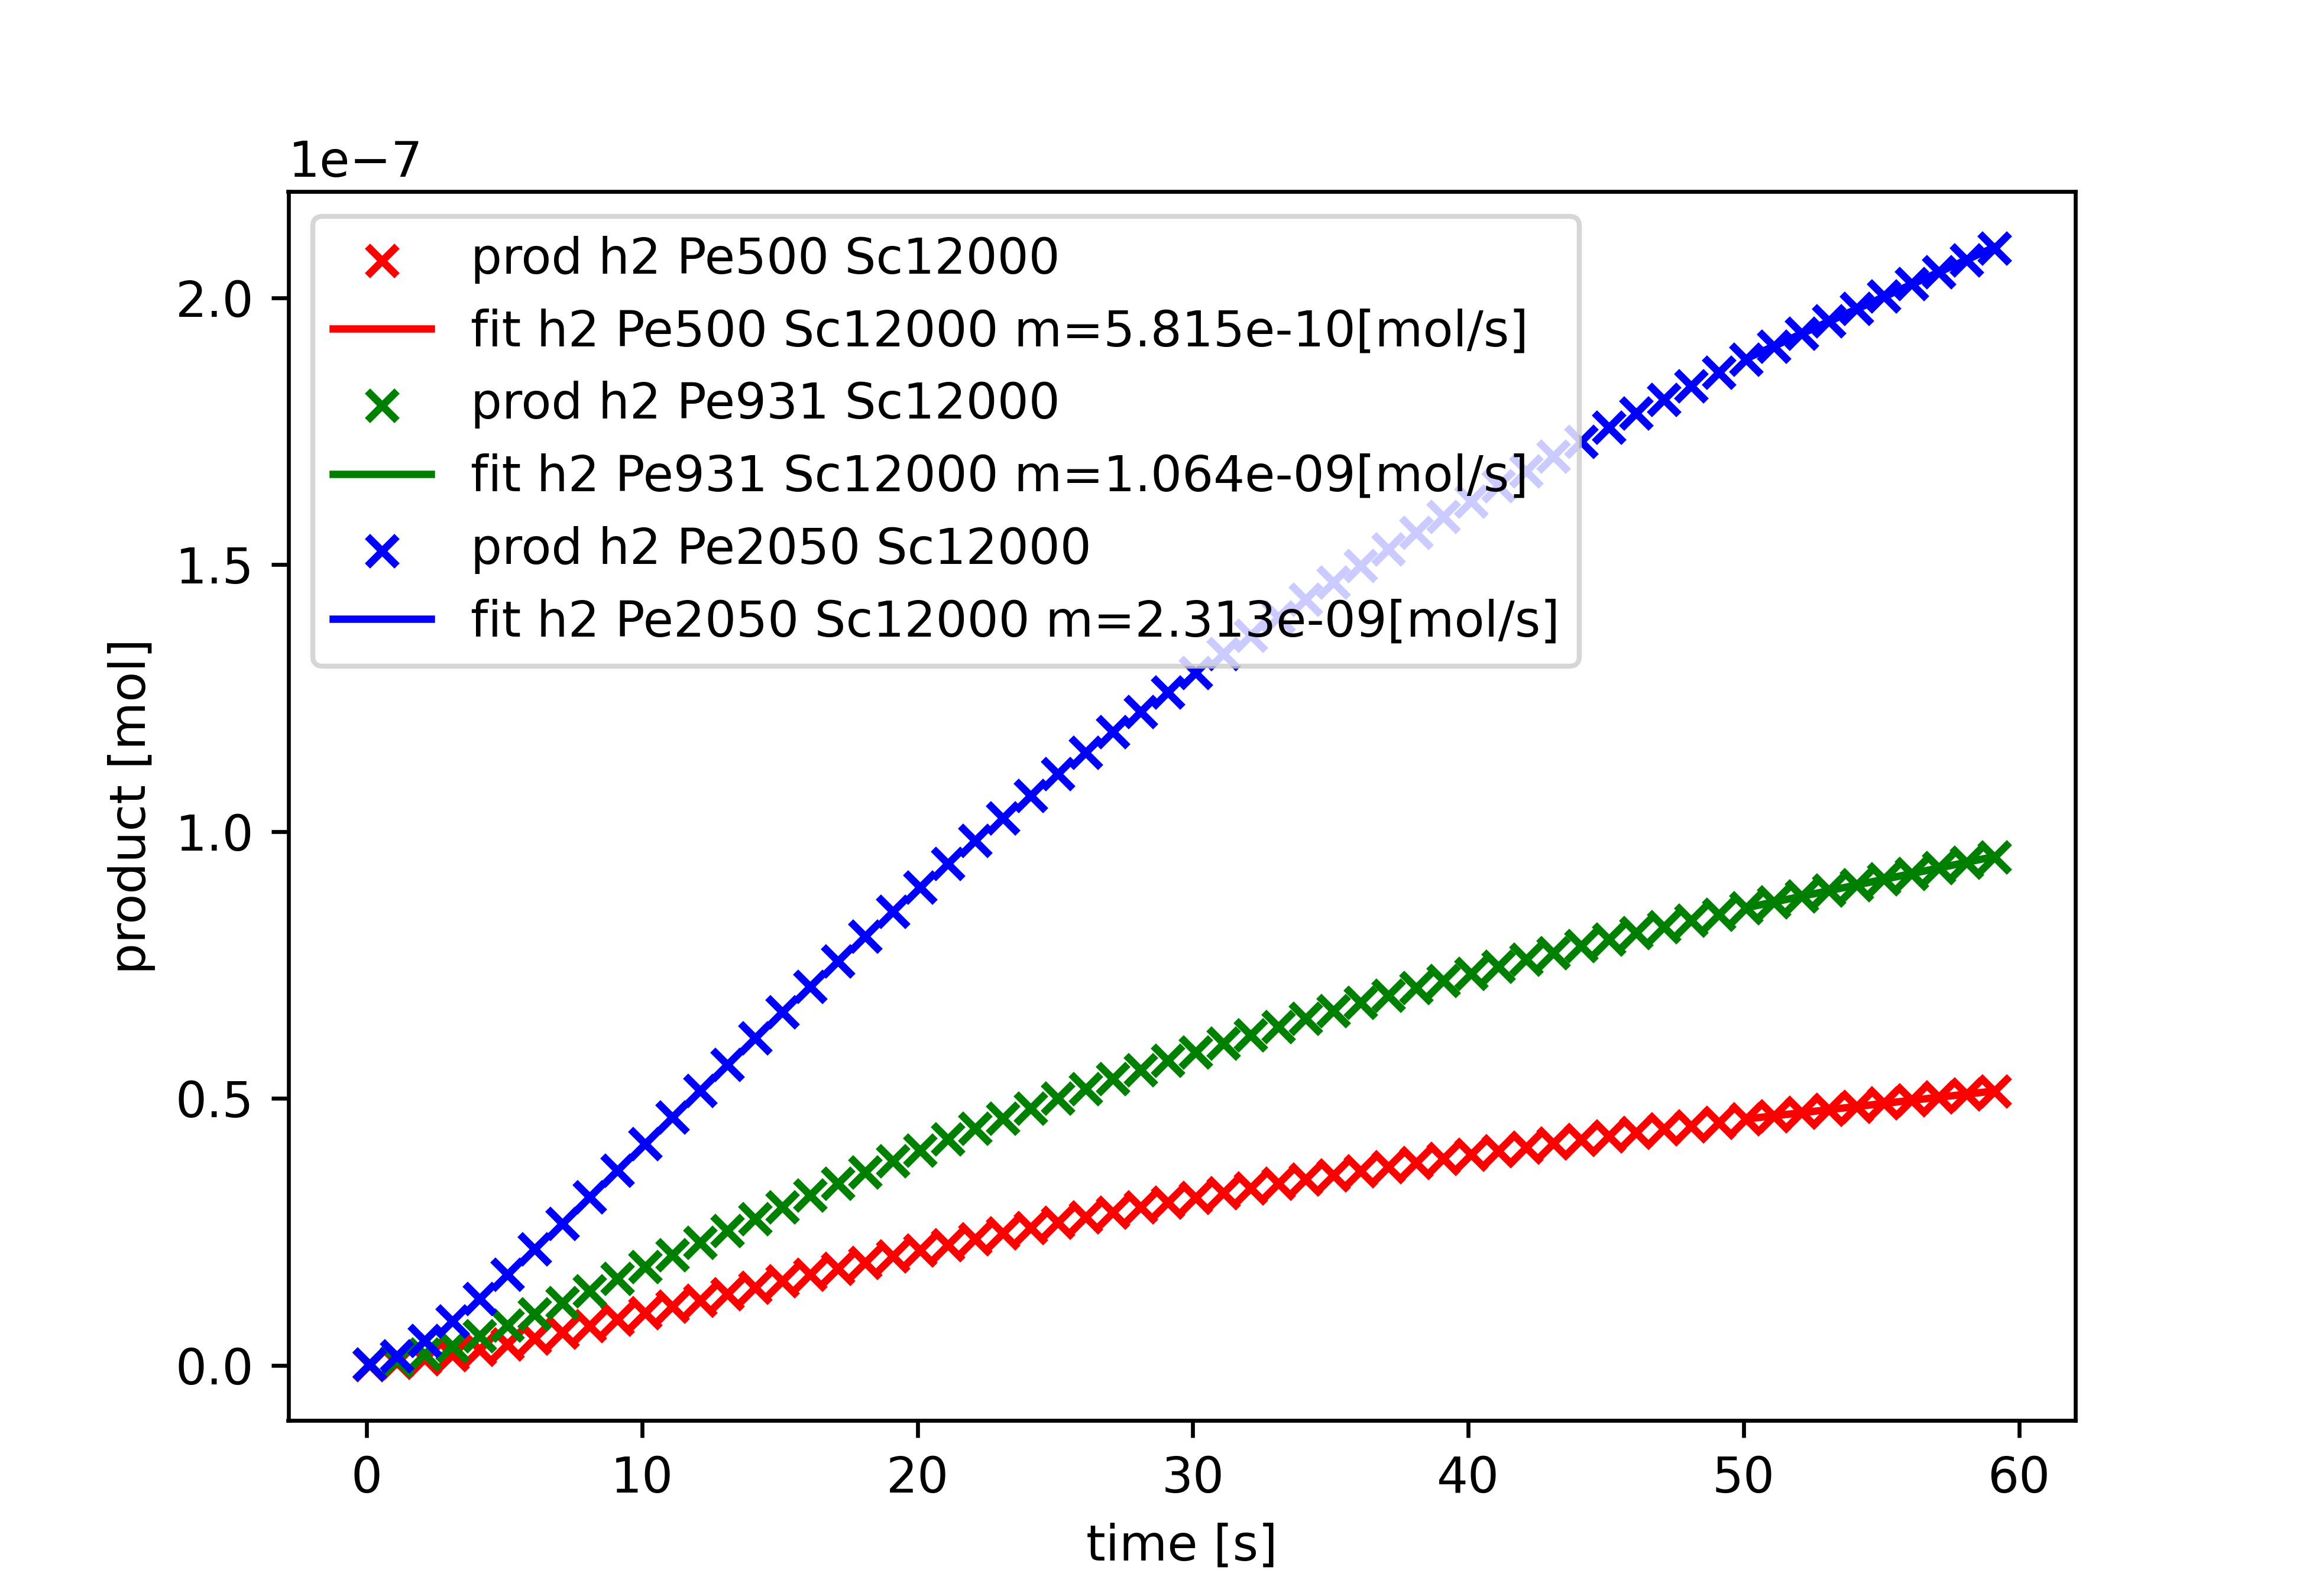
\includegraphics[width=.9\linewidth]{total_product_h2_Sc12000}
	\caption{total product for  h = 0.2mm Sc = 12000\label{fig: total_prod_h2_Sc12000}}\bigskip
	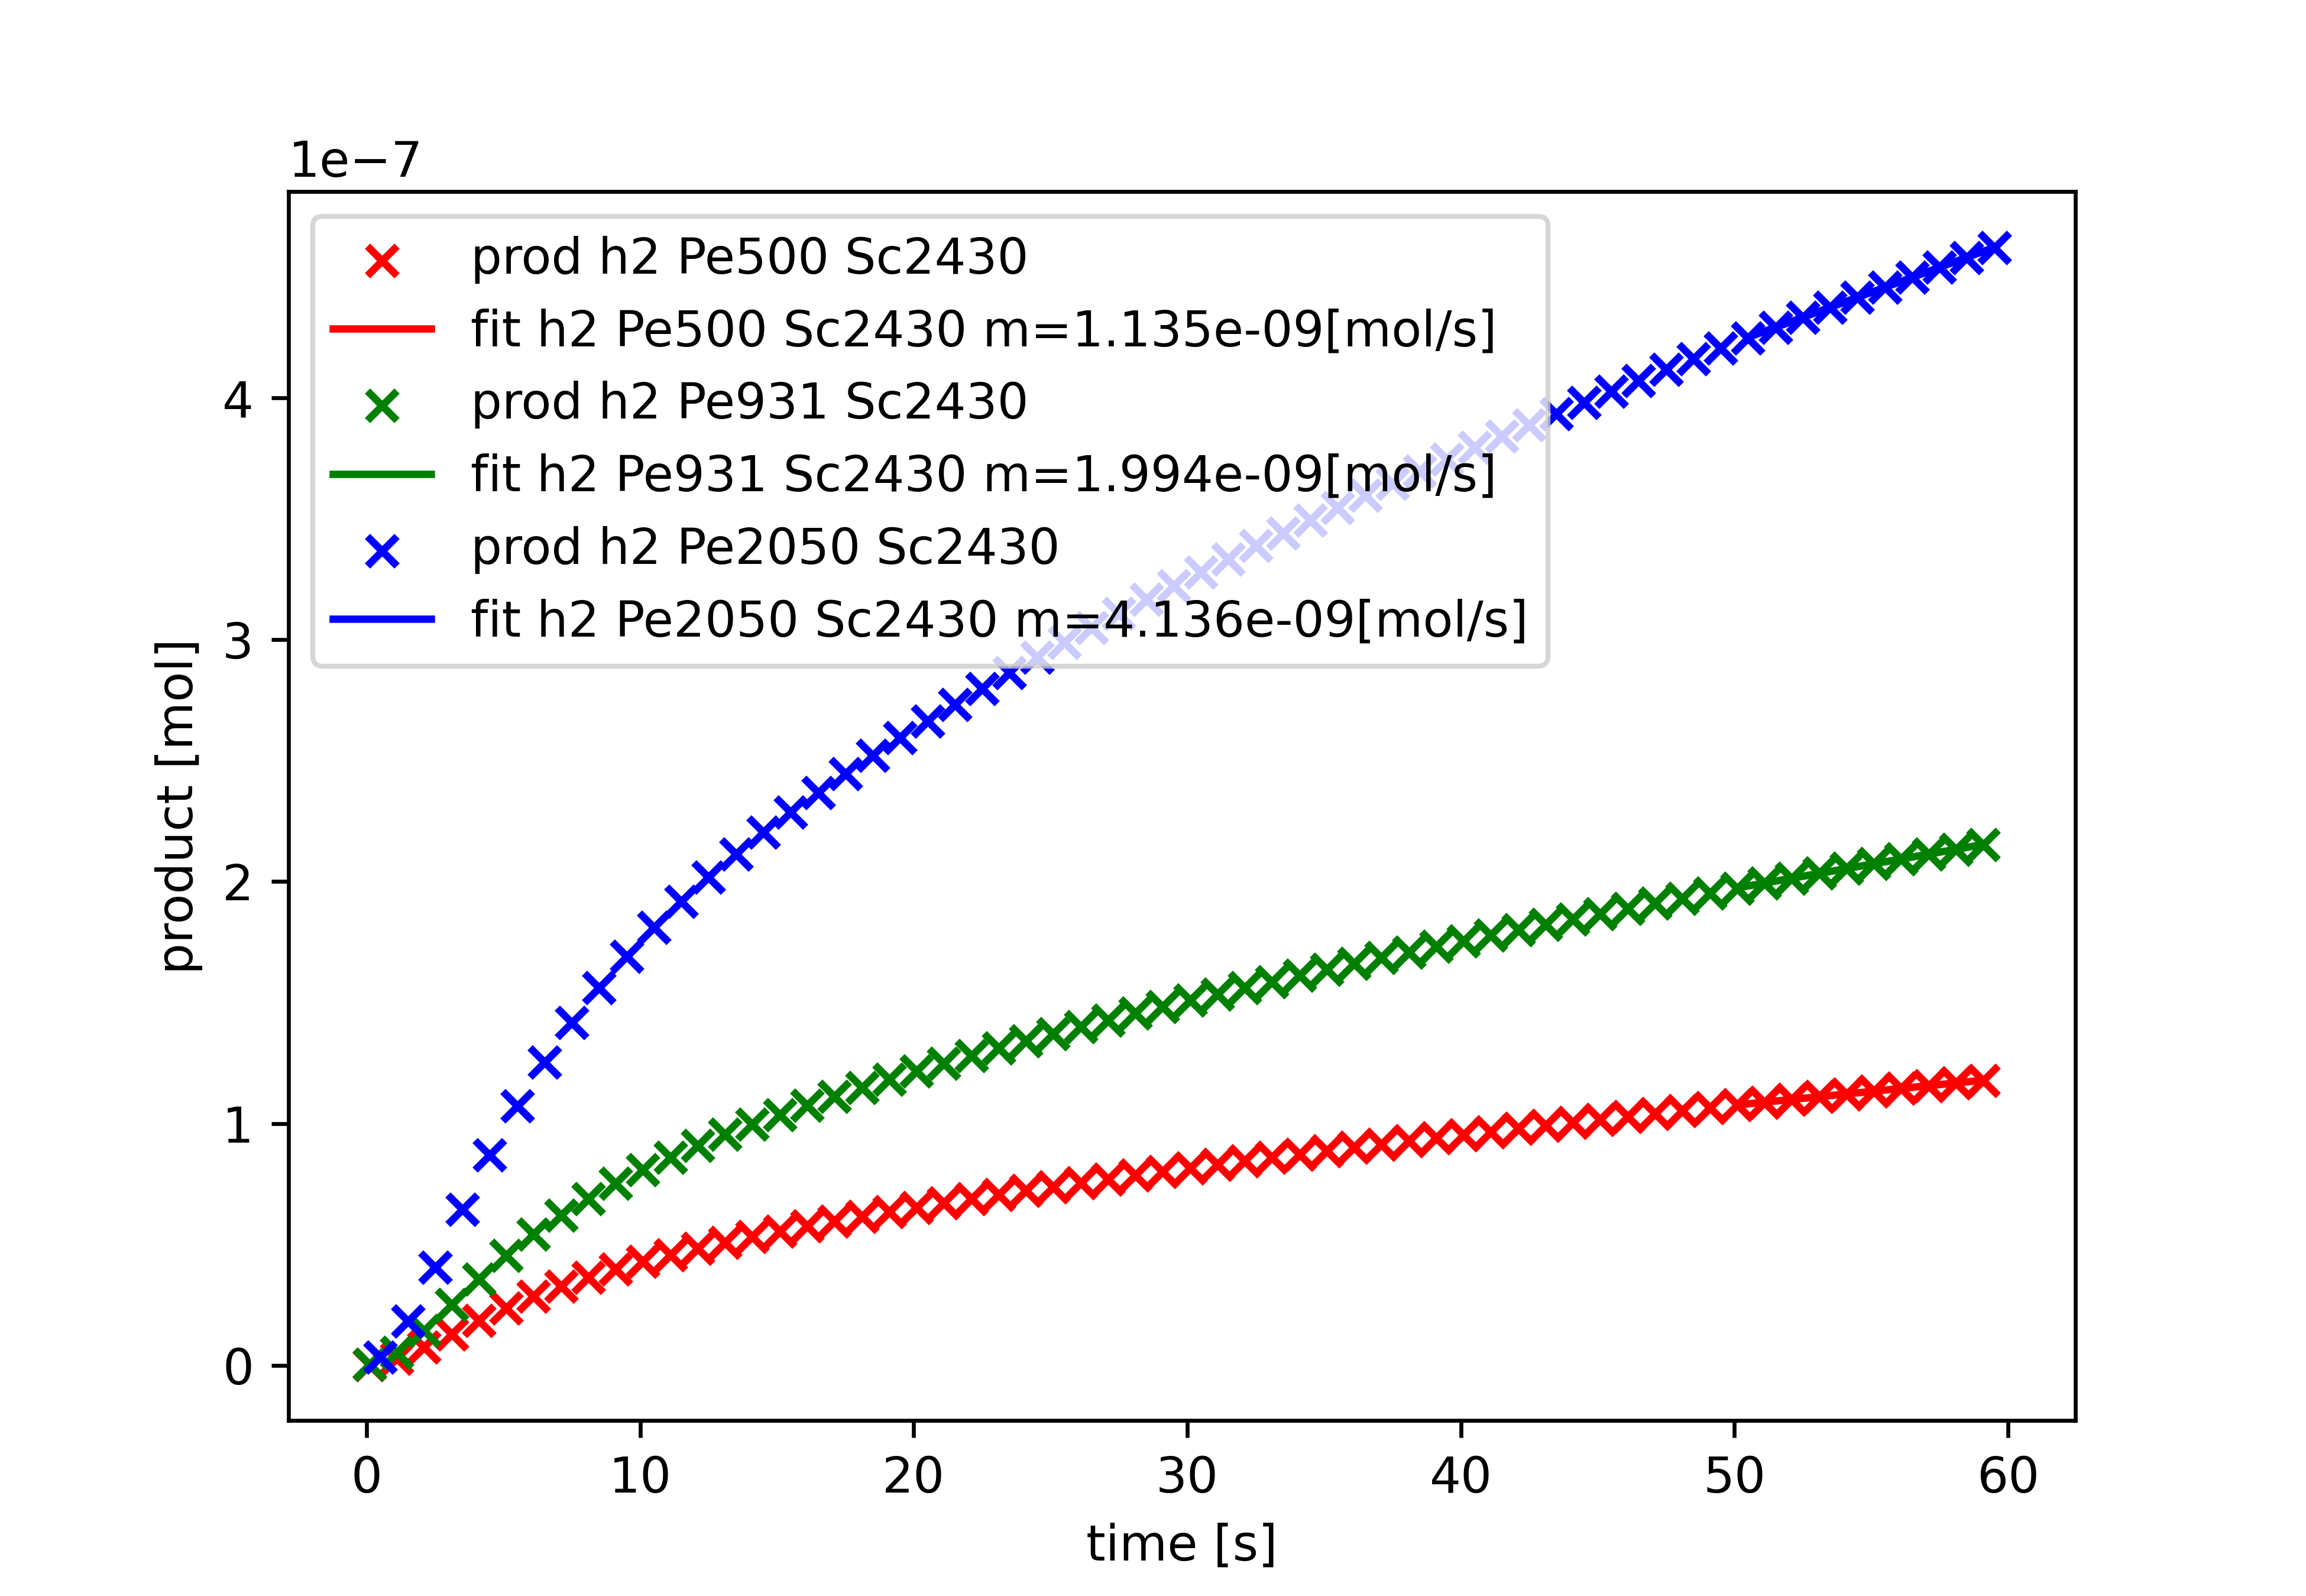
\includegraphics[width=.9\linewidth]{total_product_h2_Sc2430}
	\caption{total product for  h = 0.2mm Sc = 2430\label{fig: total_prod_h2_Sc2430}}
\end{figure}

For the case with a gap height of 0.2mm the total product formed starts with a linear growth which then slowly decays for all cases with a Schmidt number of 12000. Concluding out of this behaviour the production rate initially has a constant value that then decays over time towards its final value. This is clearly visible for the case with a Peclet number of 2050 within the $Sc = 2430$ plot. The difference when lowering the Schmidt number is that the initial constant growth in product formed increases and the decay starts earlier.
\begin{figure}[htb]
	\centering
	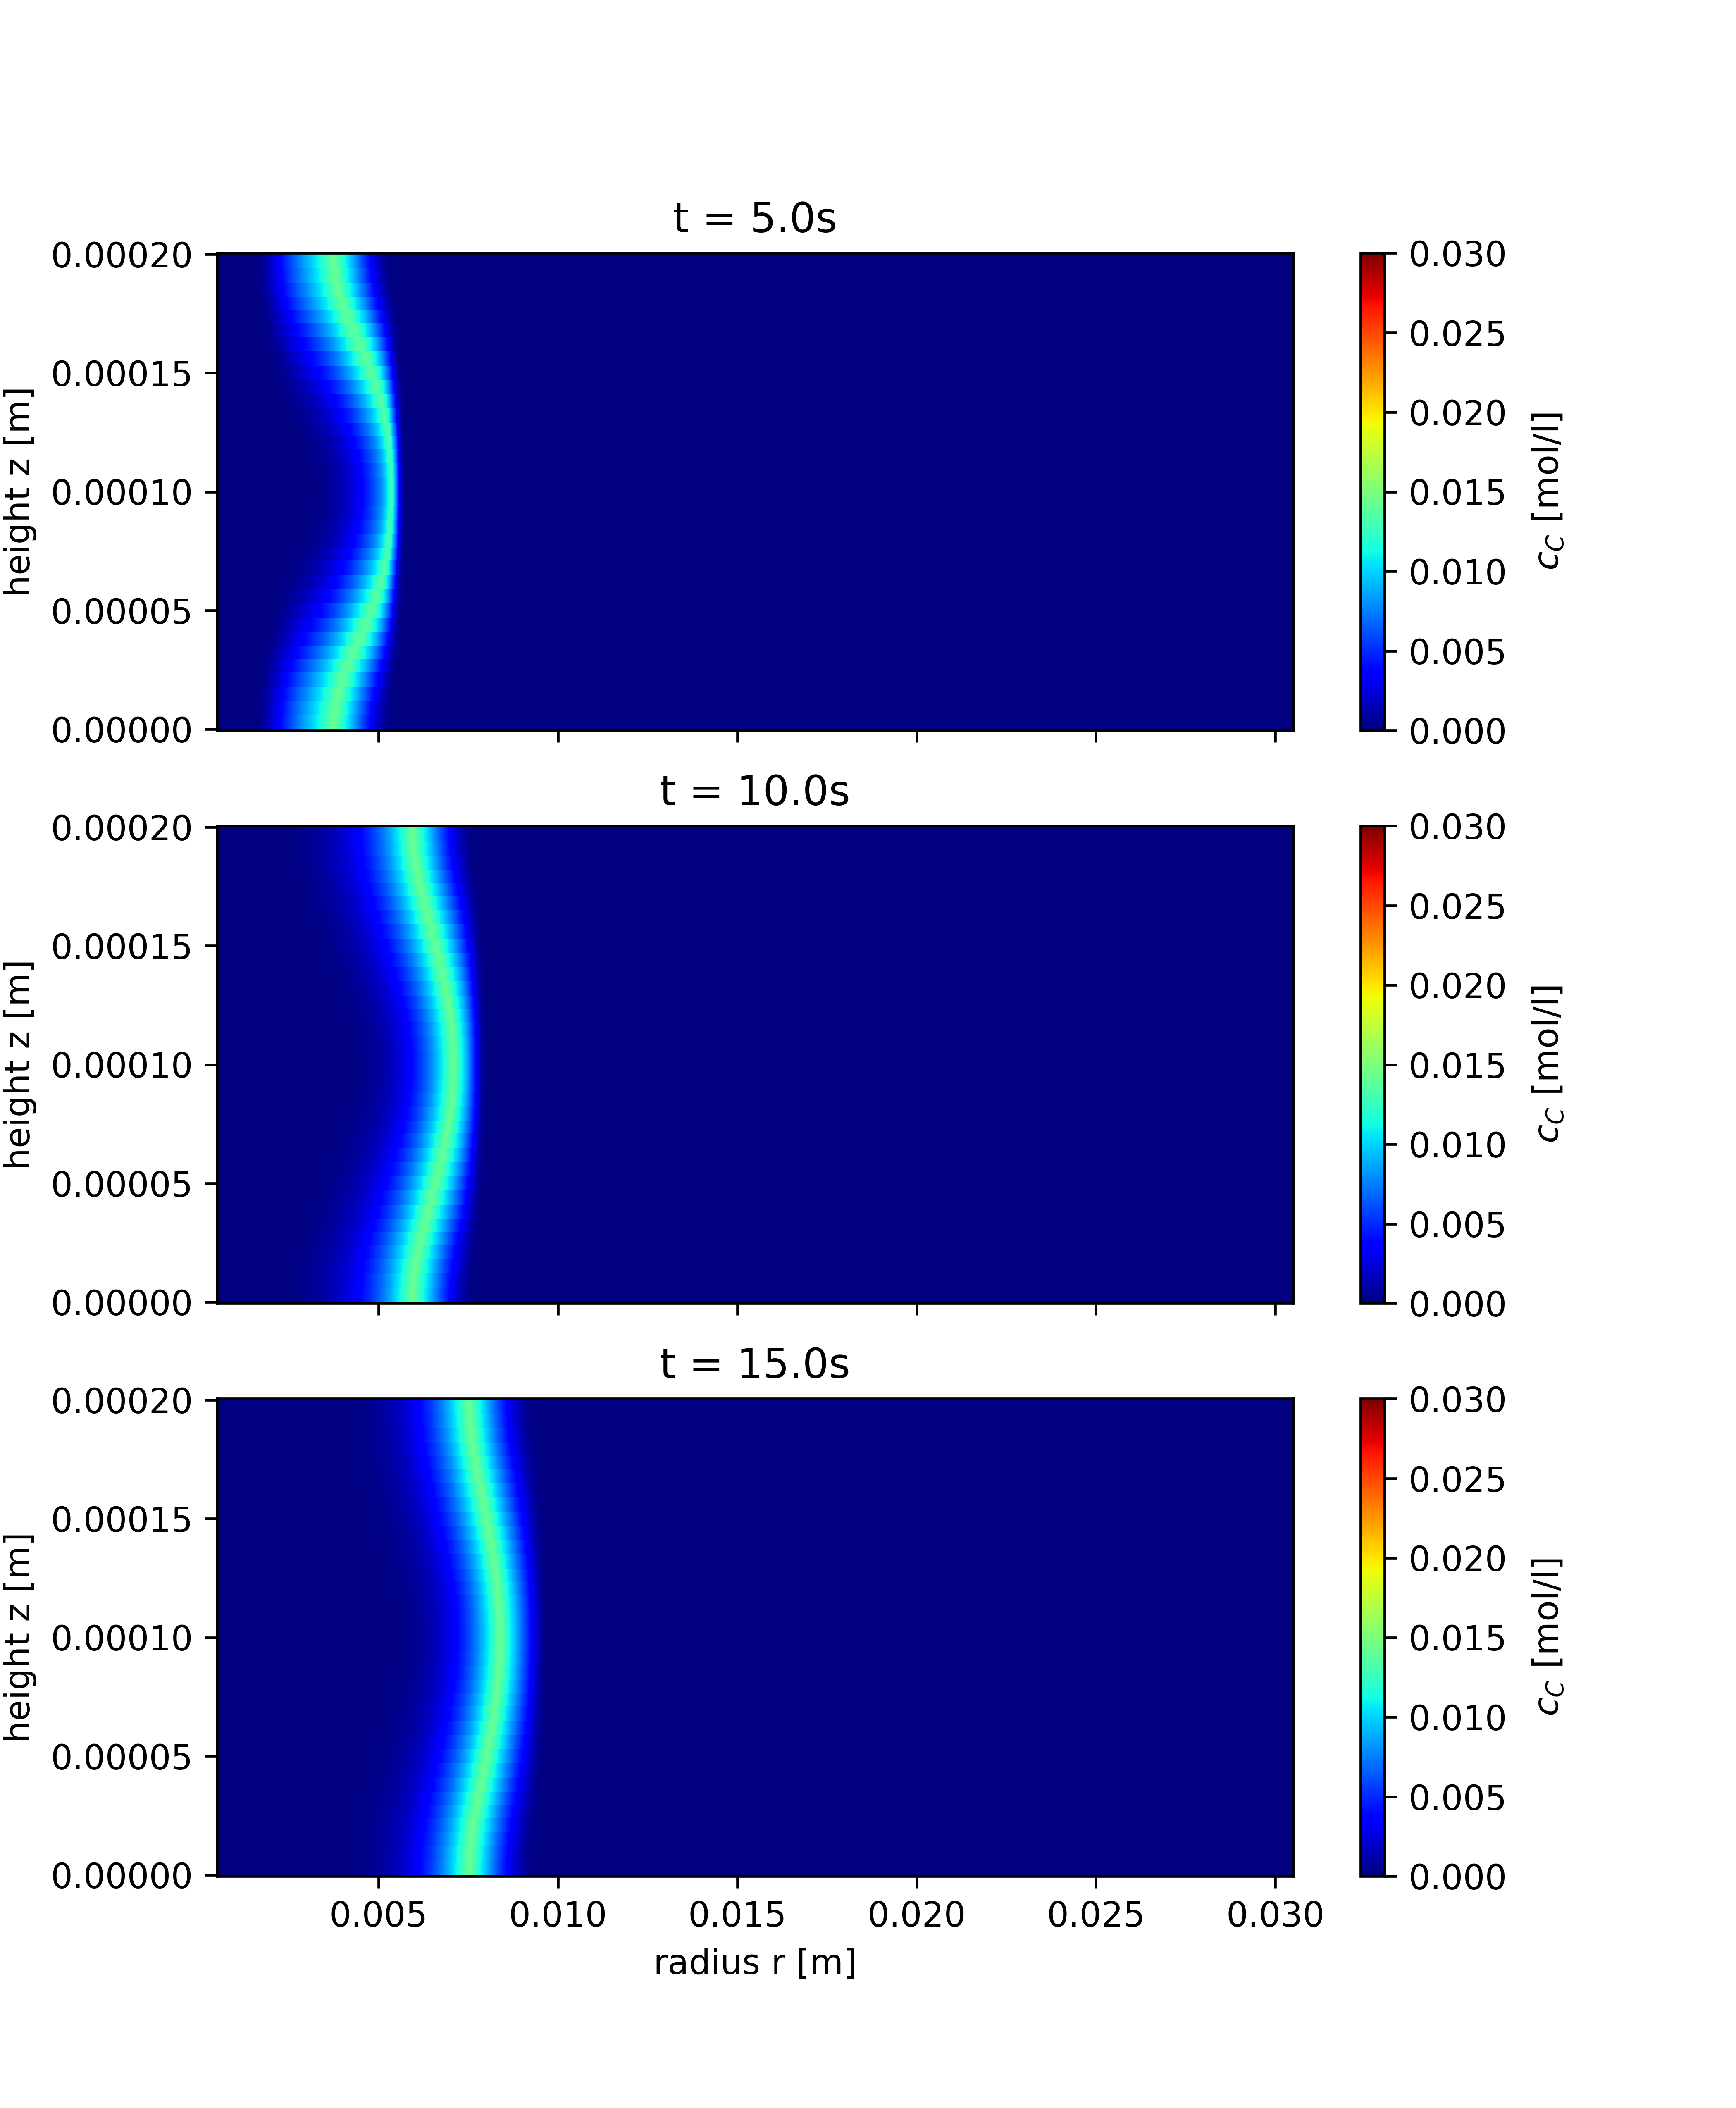
\includegraphics[width=0.7\textwidth]{field_h2r3_P205E3_S243E3_concentration-fluid_c}
	\caption{front shape for Pe = 2050 Sc = 2430}
	\label{fig: front_h2_late}
\end{figure}
In \autoref{fig: front_h2_late} the product concentration fields are shown for a time of 5 seconds which is within the phase of initial constant production rate, a time of 10 seconds which marks the point of production rate decay and a time of 15 seconds which is in the final constant phase. From these fronts it can be seen that the production rate is constantly high until the front starts to experience a more and more growing influence of diffusion. This can be seen by looking at the width and overall product concentration in front of the front. At 5 seconds the width at half the gap height is small and nearly no product is visible in the space in front of the front. This can explain the initially higher production rate because the front is still developing its shape at that time. At 10 seconds that does change. The FWHMHGH has gained the same shape is the widths above and below it and a slight amount of product starts appearing at coordinates with higher radial values than the fronts front. When this point in time is reached the front is established within the hole gap so the production rate slows down. Apparently the described effect is not clearly visible within the widths plot of this case as shown in \autoref{fig: front_width_pos_h2_Sc2430} due to the way the FWHMHGH is calculated. From the widths plot it is visible that the middle width stops growing at the time of 10 seconds when the diffusive influence starts raising. That could be used as in indication as well that diffusion starts affecting the front.

\begin{figure}[htbp]
	\centering
	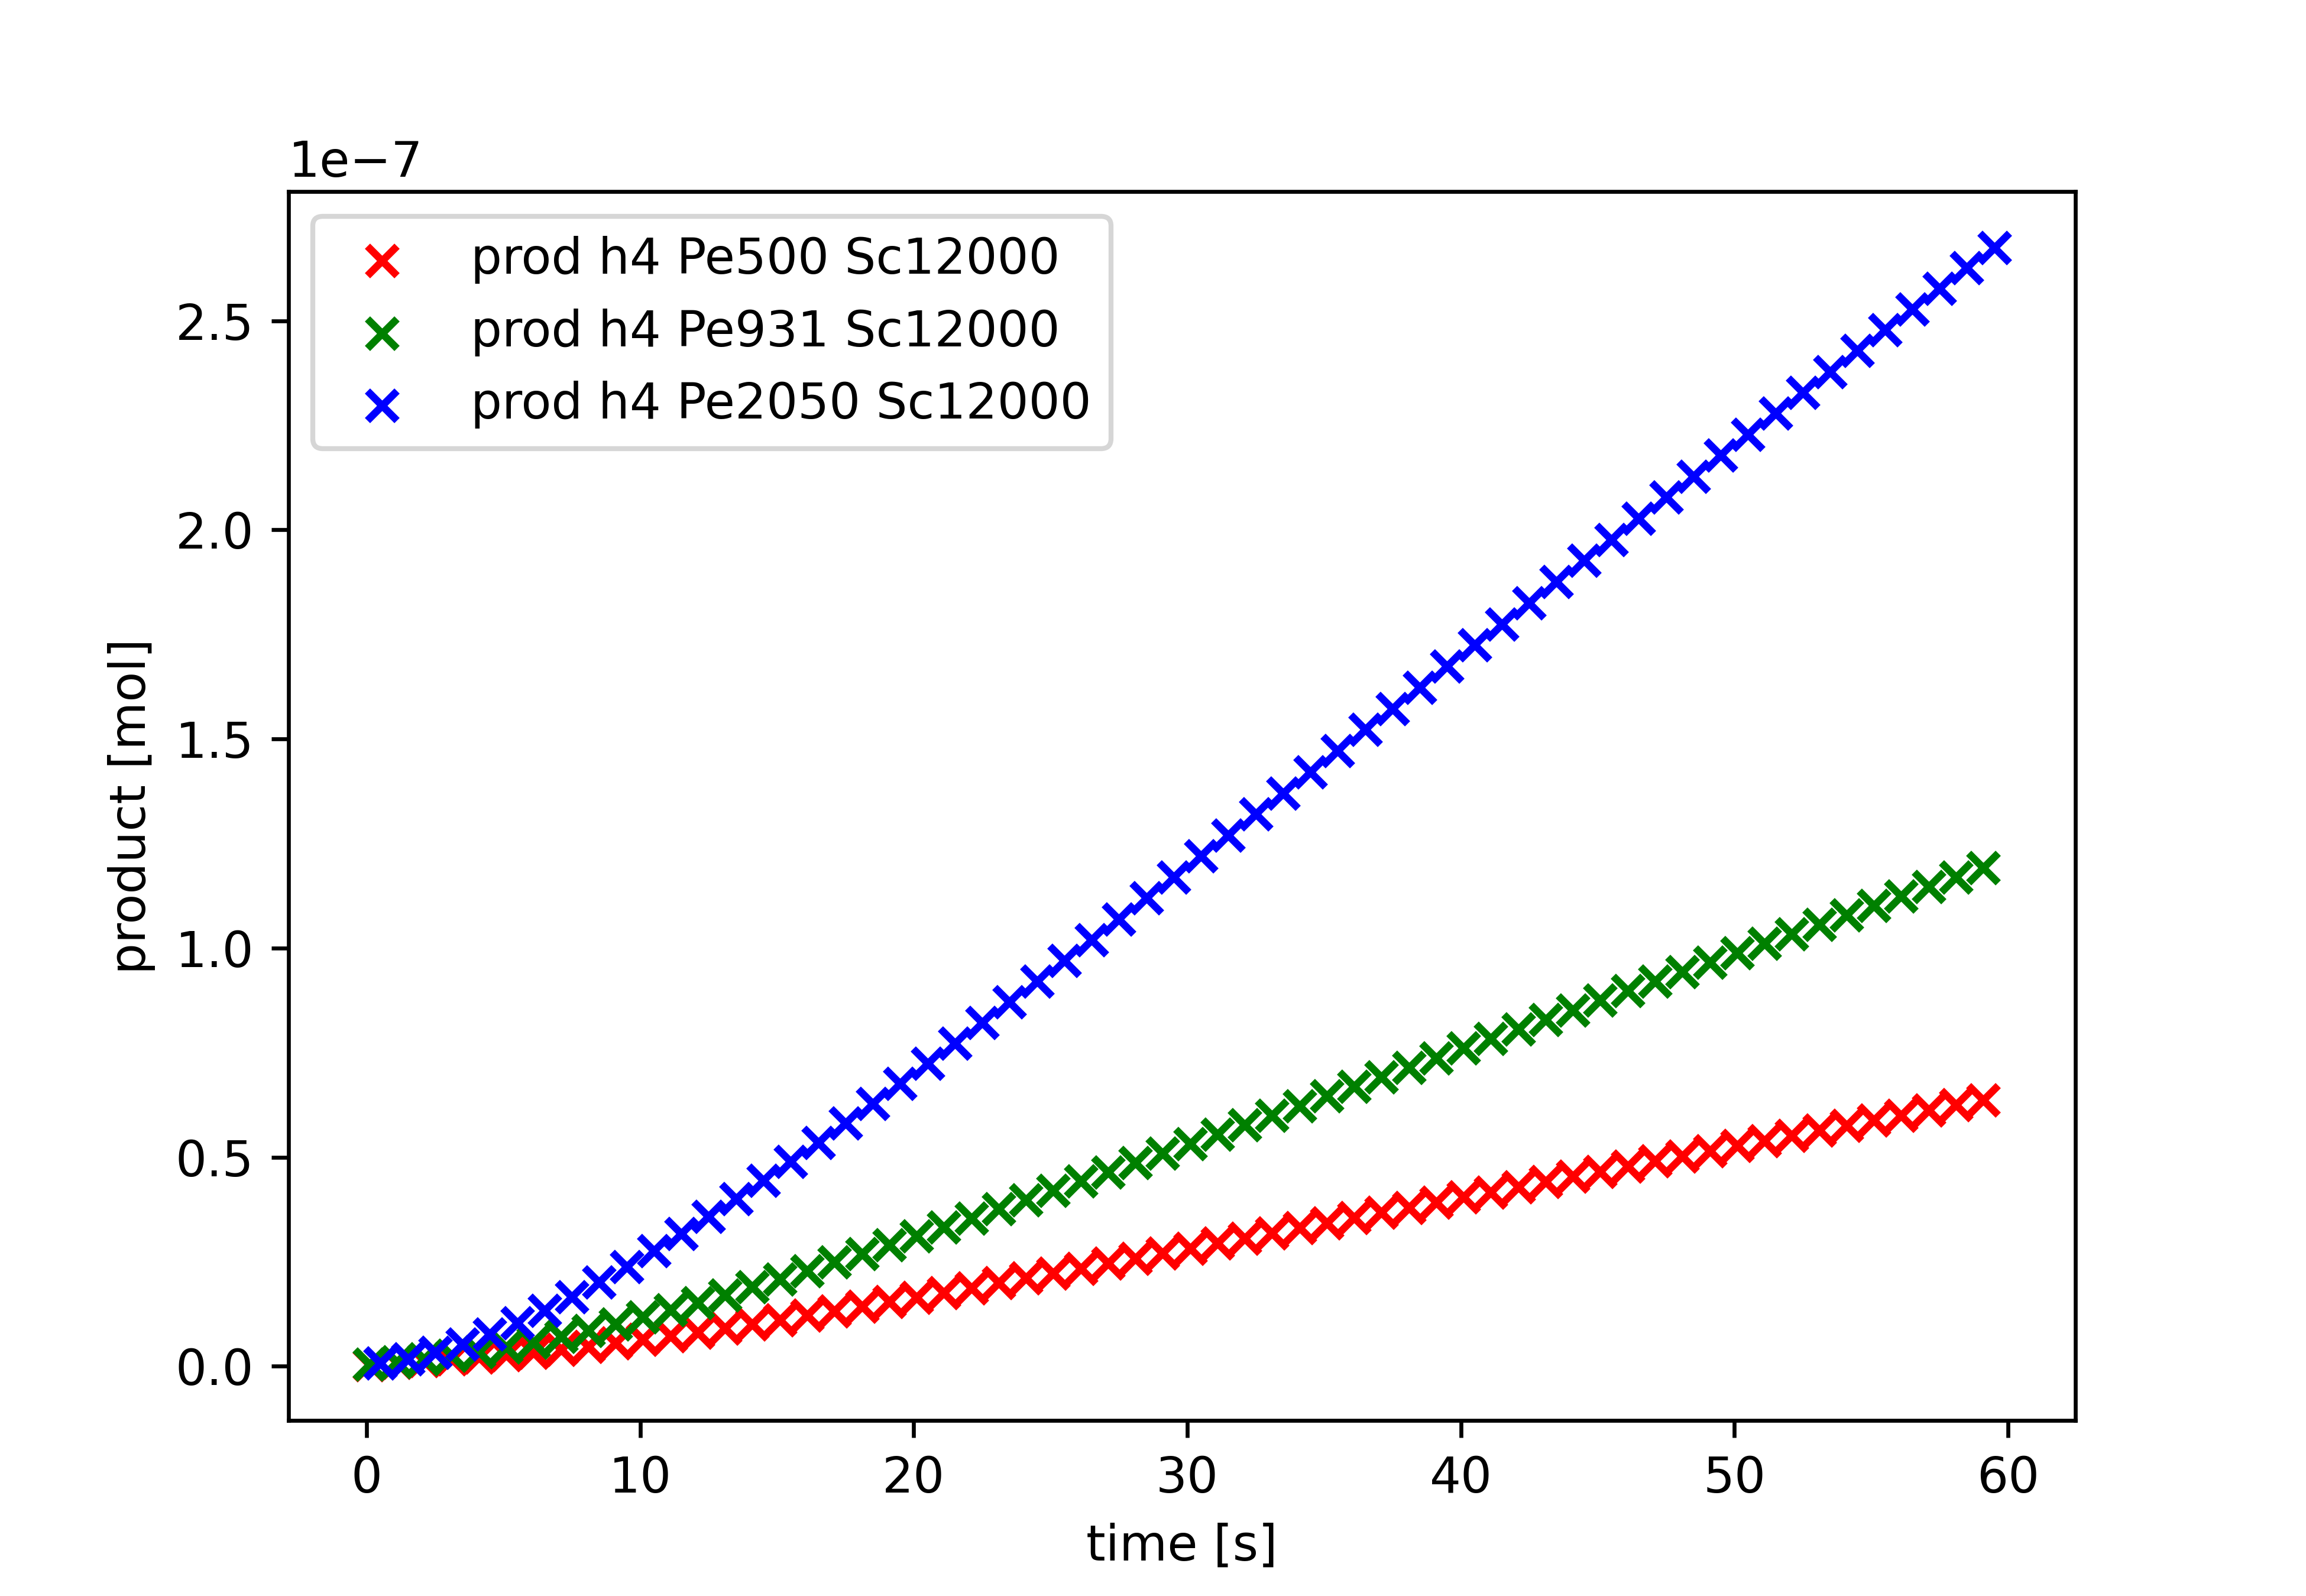
\includegraphics[width=.9\linewidth]{total_product_h4_Sc12000}
	\caption{total product for  h = 0.4mm Sc = 12000\label{fig: total_prod_h4_Sc12000}}\bigskip
	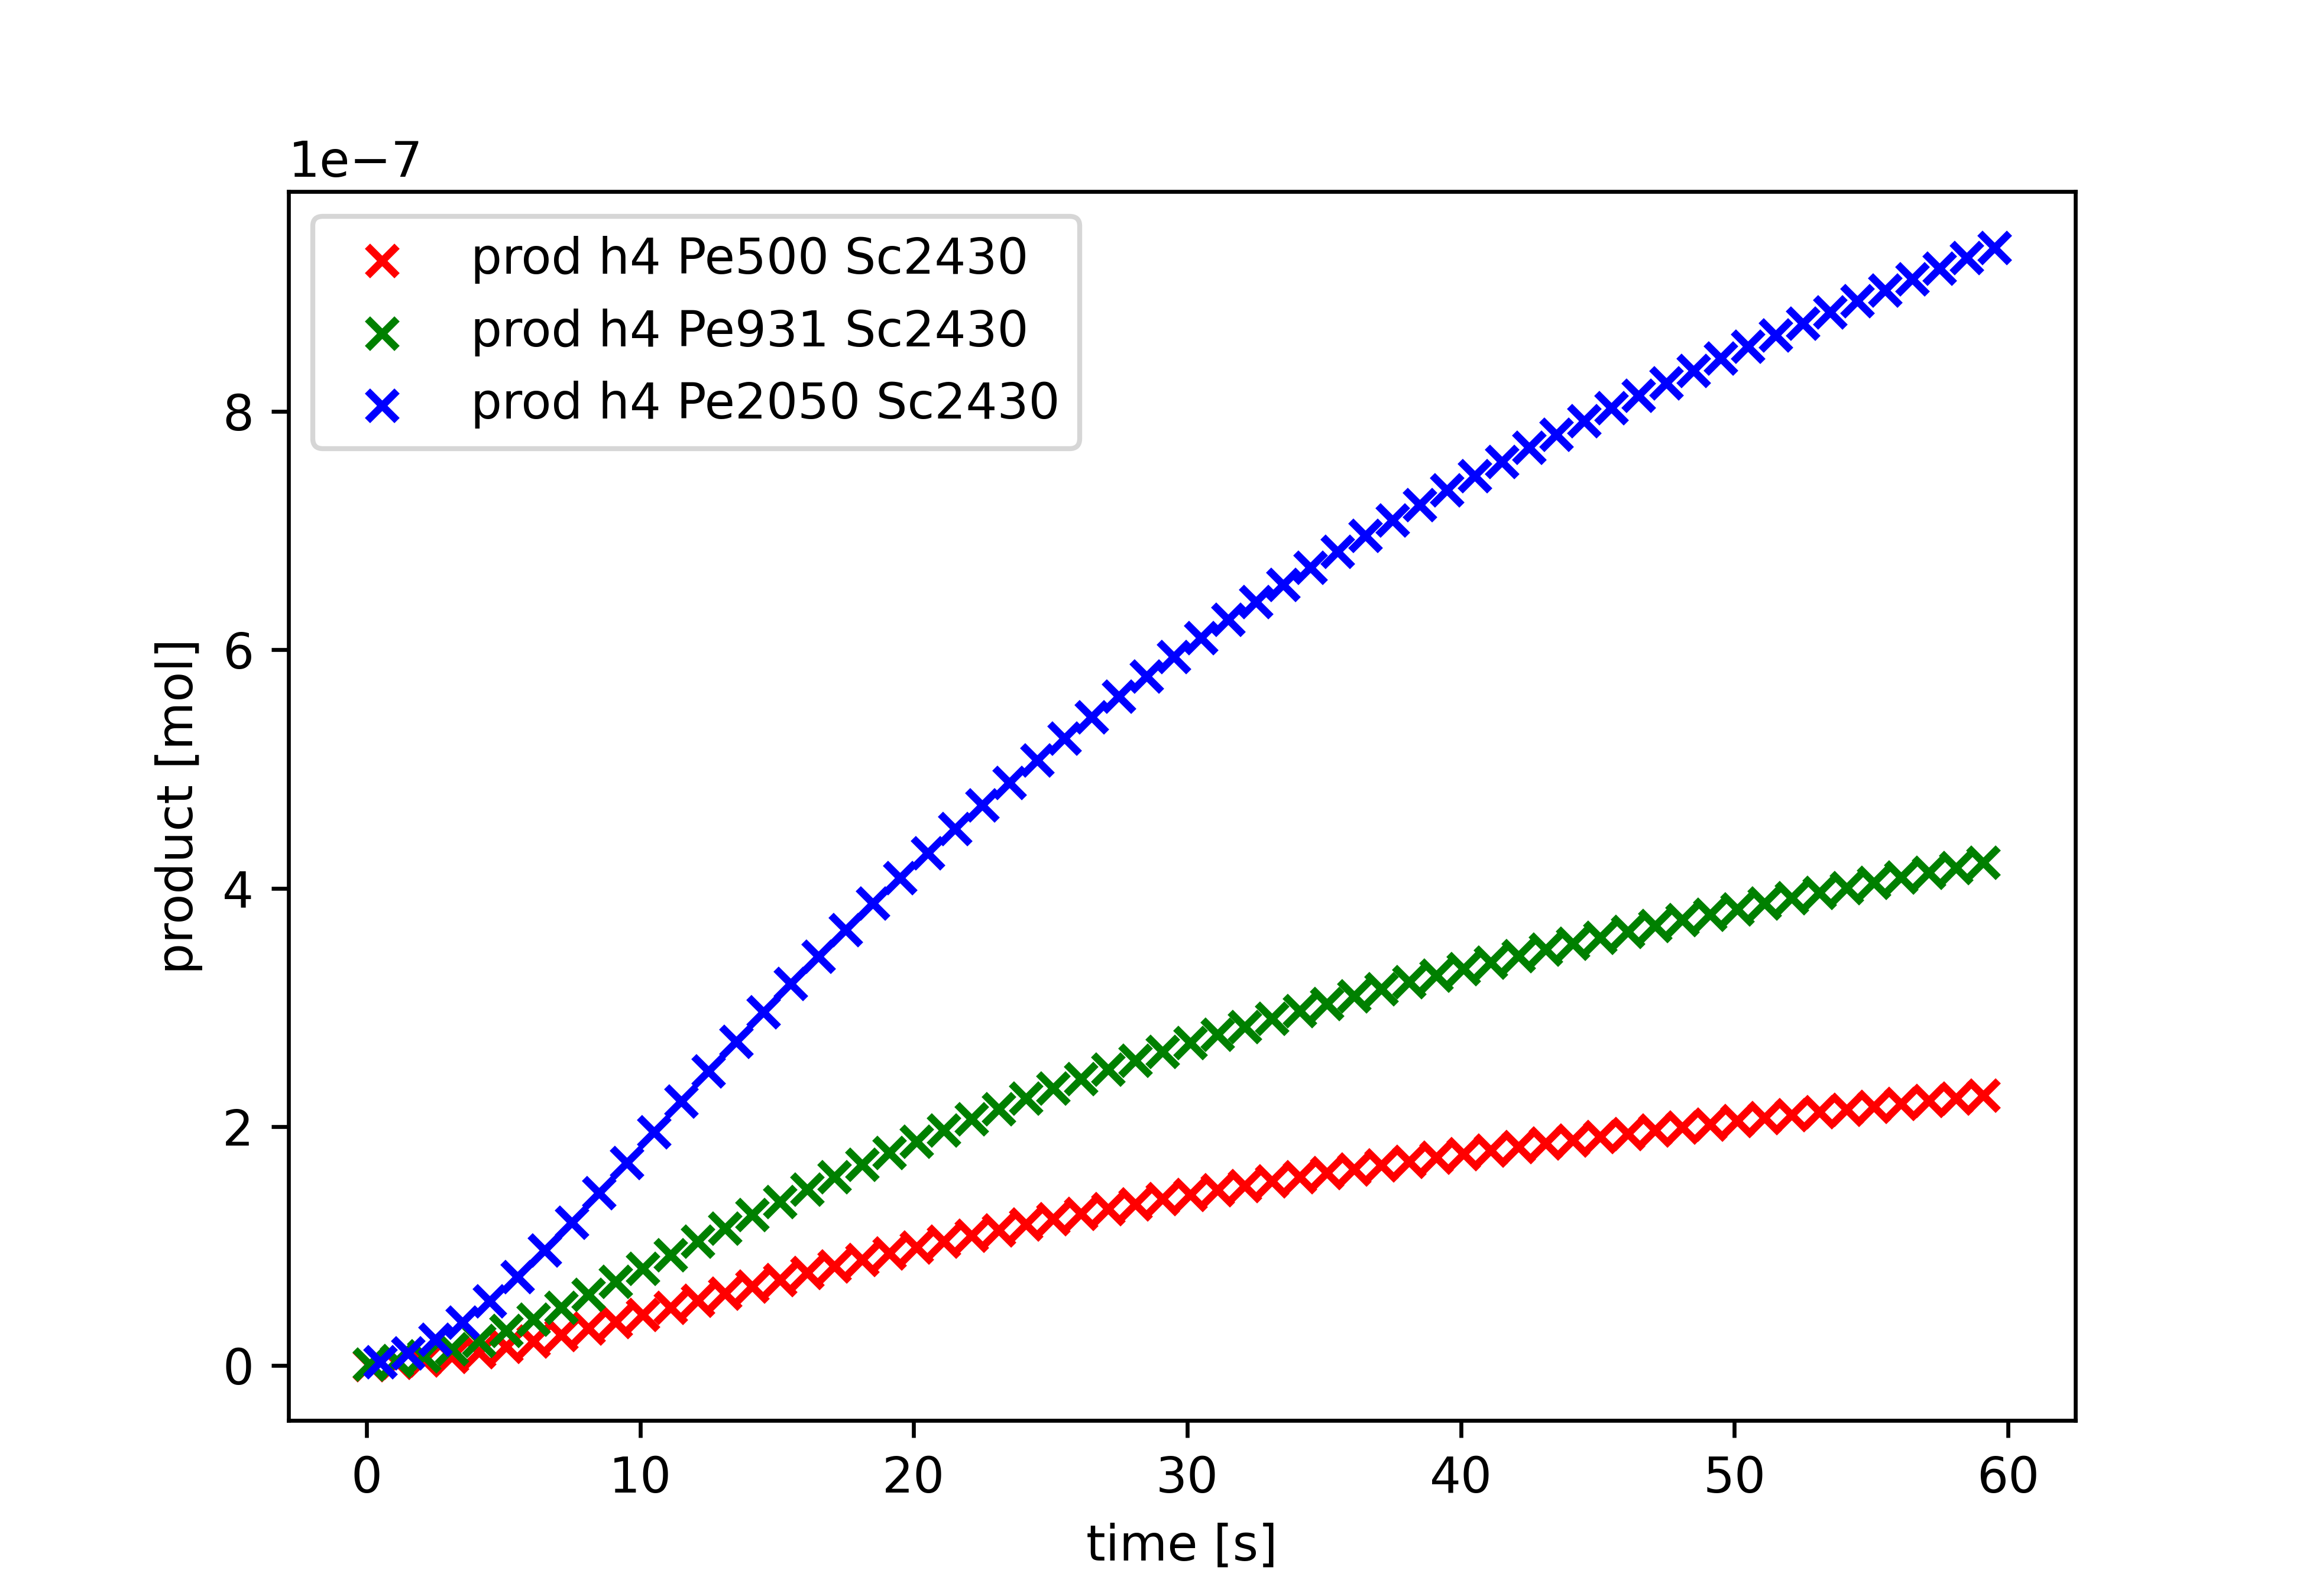
\includegraphics[width=.9\linewidth]{total_product_h4_Sc2430}
	\caption{total product for  h = 0.4mm Sc = 2430\label{fig: total_prod_h4_Sc2430}}
\end{figure}

The total product created seems to follow the same general behaviour for the cases with a gap height of 0.4mm compared to the 0.2mm ones. For the lower Schmidt number the graphs look very similar when comparing \autoref{fig: total_prod_h4_Sc2430} and \autoref{fig: total_prod_h2_Sc2430}. The values are higher for the 0.4mm case but that is a result of the higher gap height and therefore higher volumetric flow through the reactor. The amount of product created is highly influenced by the Peclet number. With approximately doubling the Peclet number between different cases for the same Schmidt number the total product produced at 60 seconds goes up by a bit more than a factor of 2. That can be seen when comparing the cases for all different gap heights. That results are directly linked to the different input velocities that can be taken from \autoref{tab: cases}. The production rate is driven towards a constant value at later time stages. This is because within a radial case the fronts surface area always grows when the front is travelling through the reactor. Therefore new educts are always touching the existing front so the reaction keeps on taking place. In Addition to the growing surface area the front widens so the new educt needs to diffuse through the existing front to reach it's reaction partner. The distance this diffusive process needs to bridge is dependent on the educts concentration values. From \autoref{fig: pos_h4_peaks}(a) it can be seen that the fronts products concentration values do not reach the maximum value possible of 0.03 $ \frac{\text{mol}}{\text{l}} $. As from the plot representing the $ c_A $ values it becomes clear that the distance the species $B$ needs to travel through the front to meet its reaction partner $A$ increases by time. That is another reason why the production rate decreases at later time stages.
\begin{figure}[htbp]
	\centering
	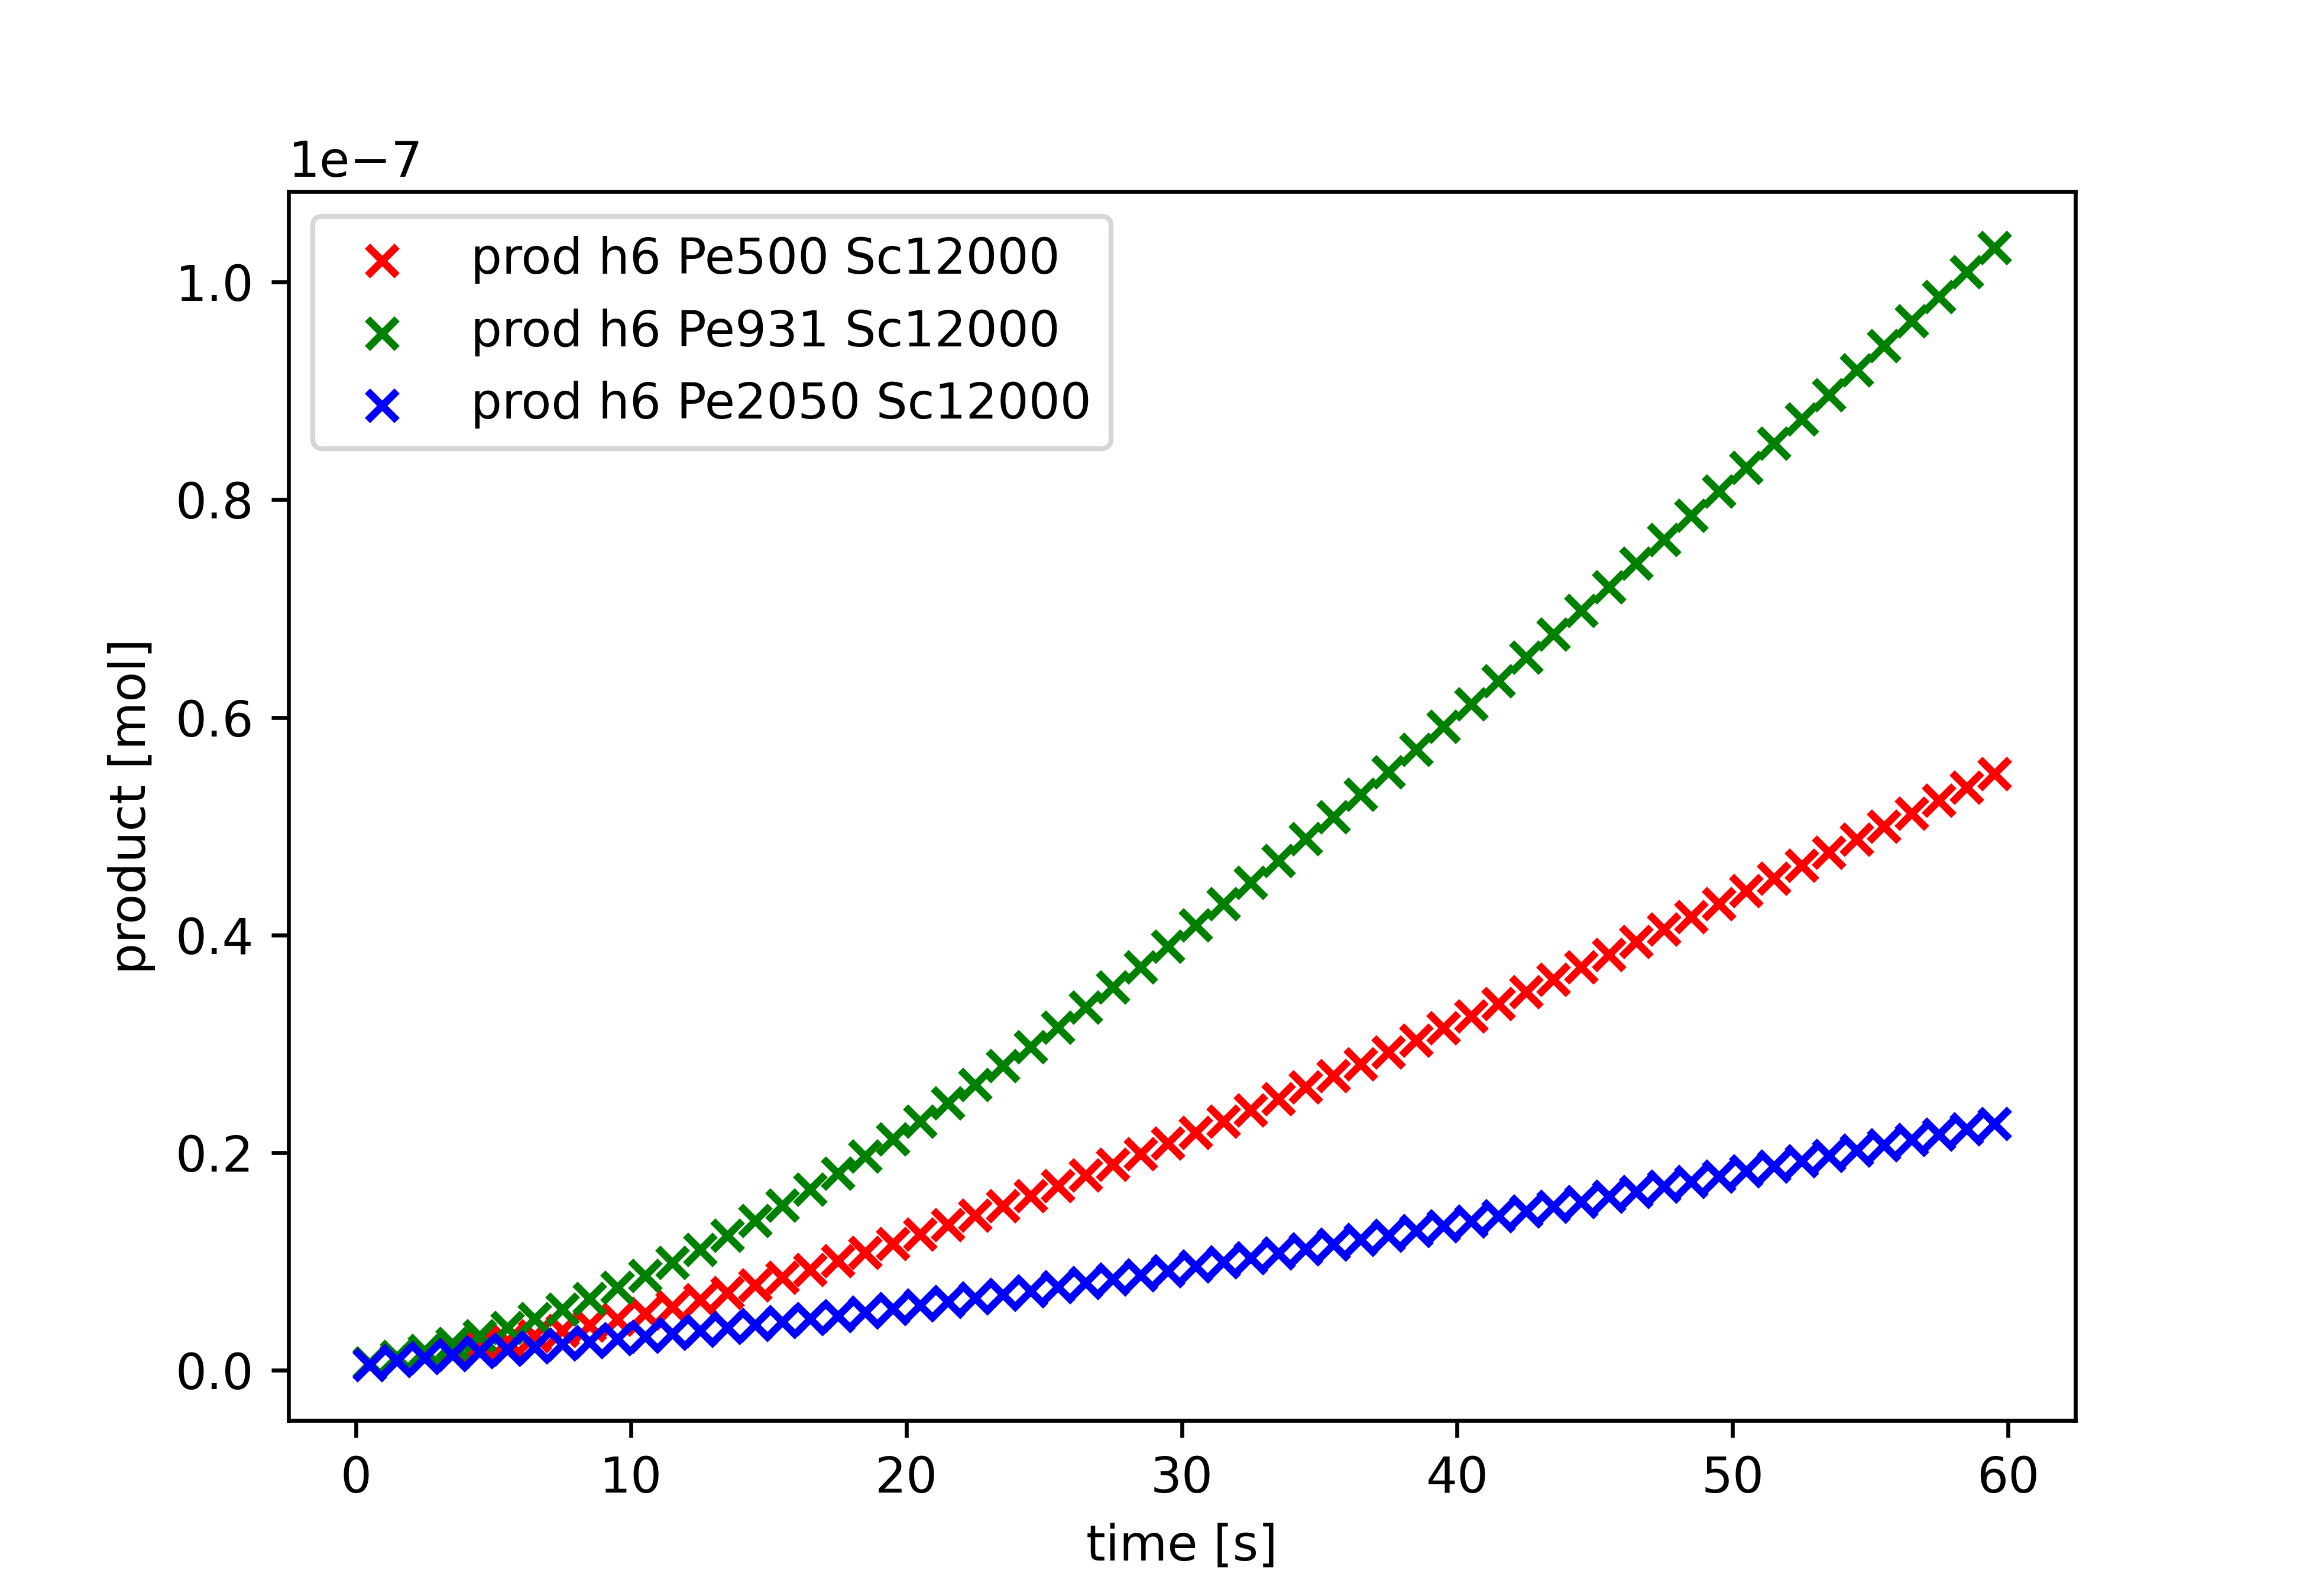
\includegraphics[width=.9\linewidth]{total_product_h6_Sc12000}
	\caption{total product for  h = 0.6mm Sc = 12000\label{fig: total_prod_h6_Sc12000}}\bigskip
	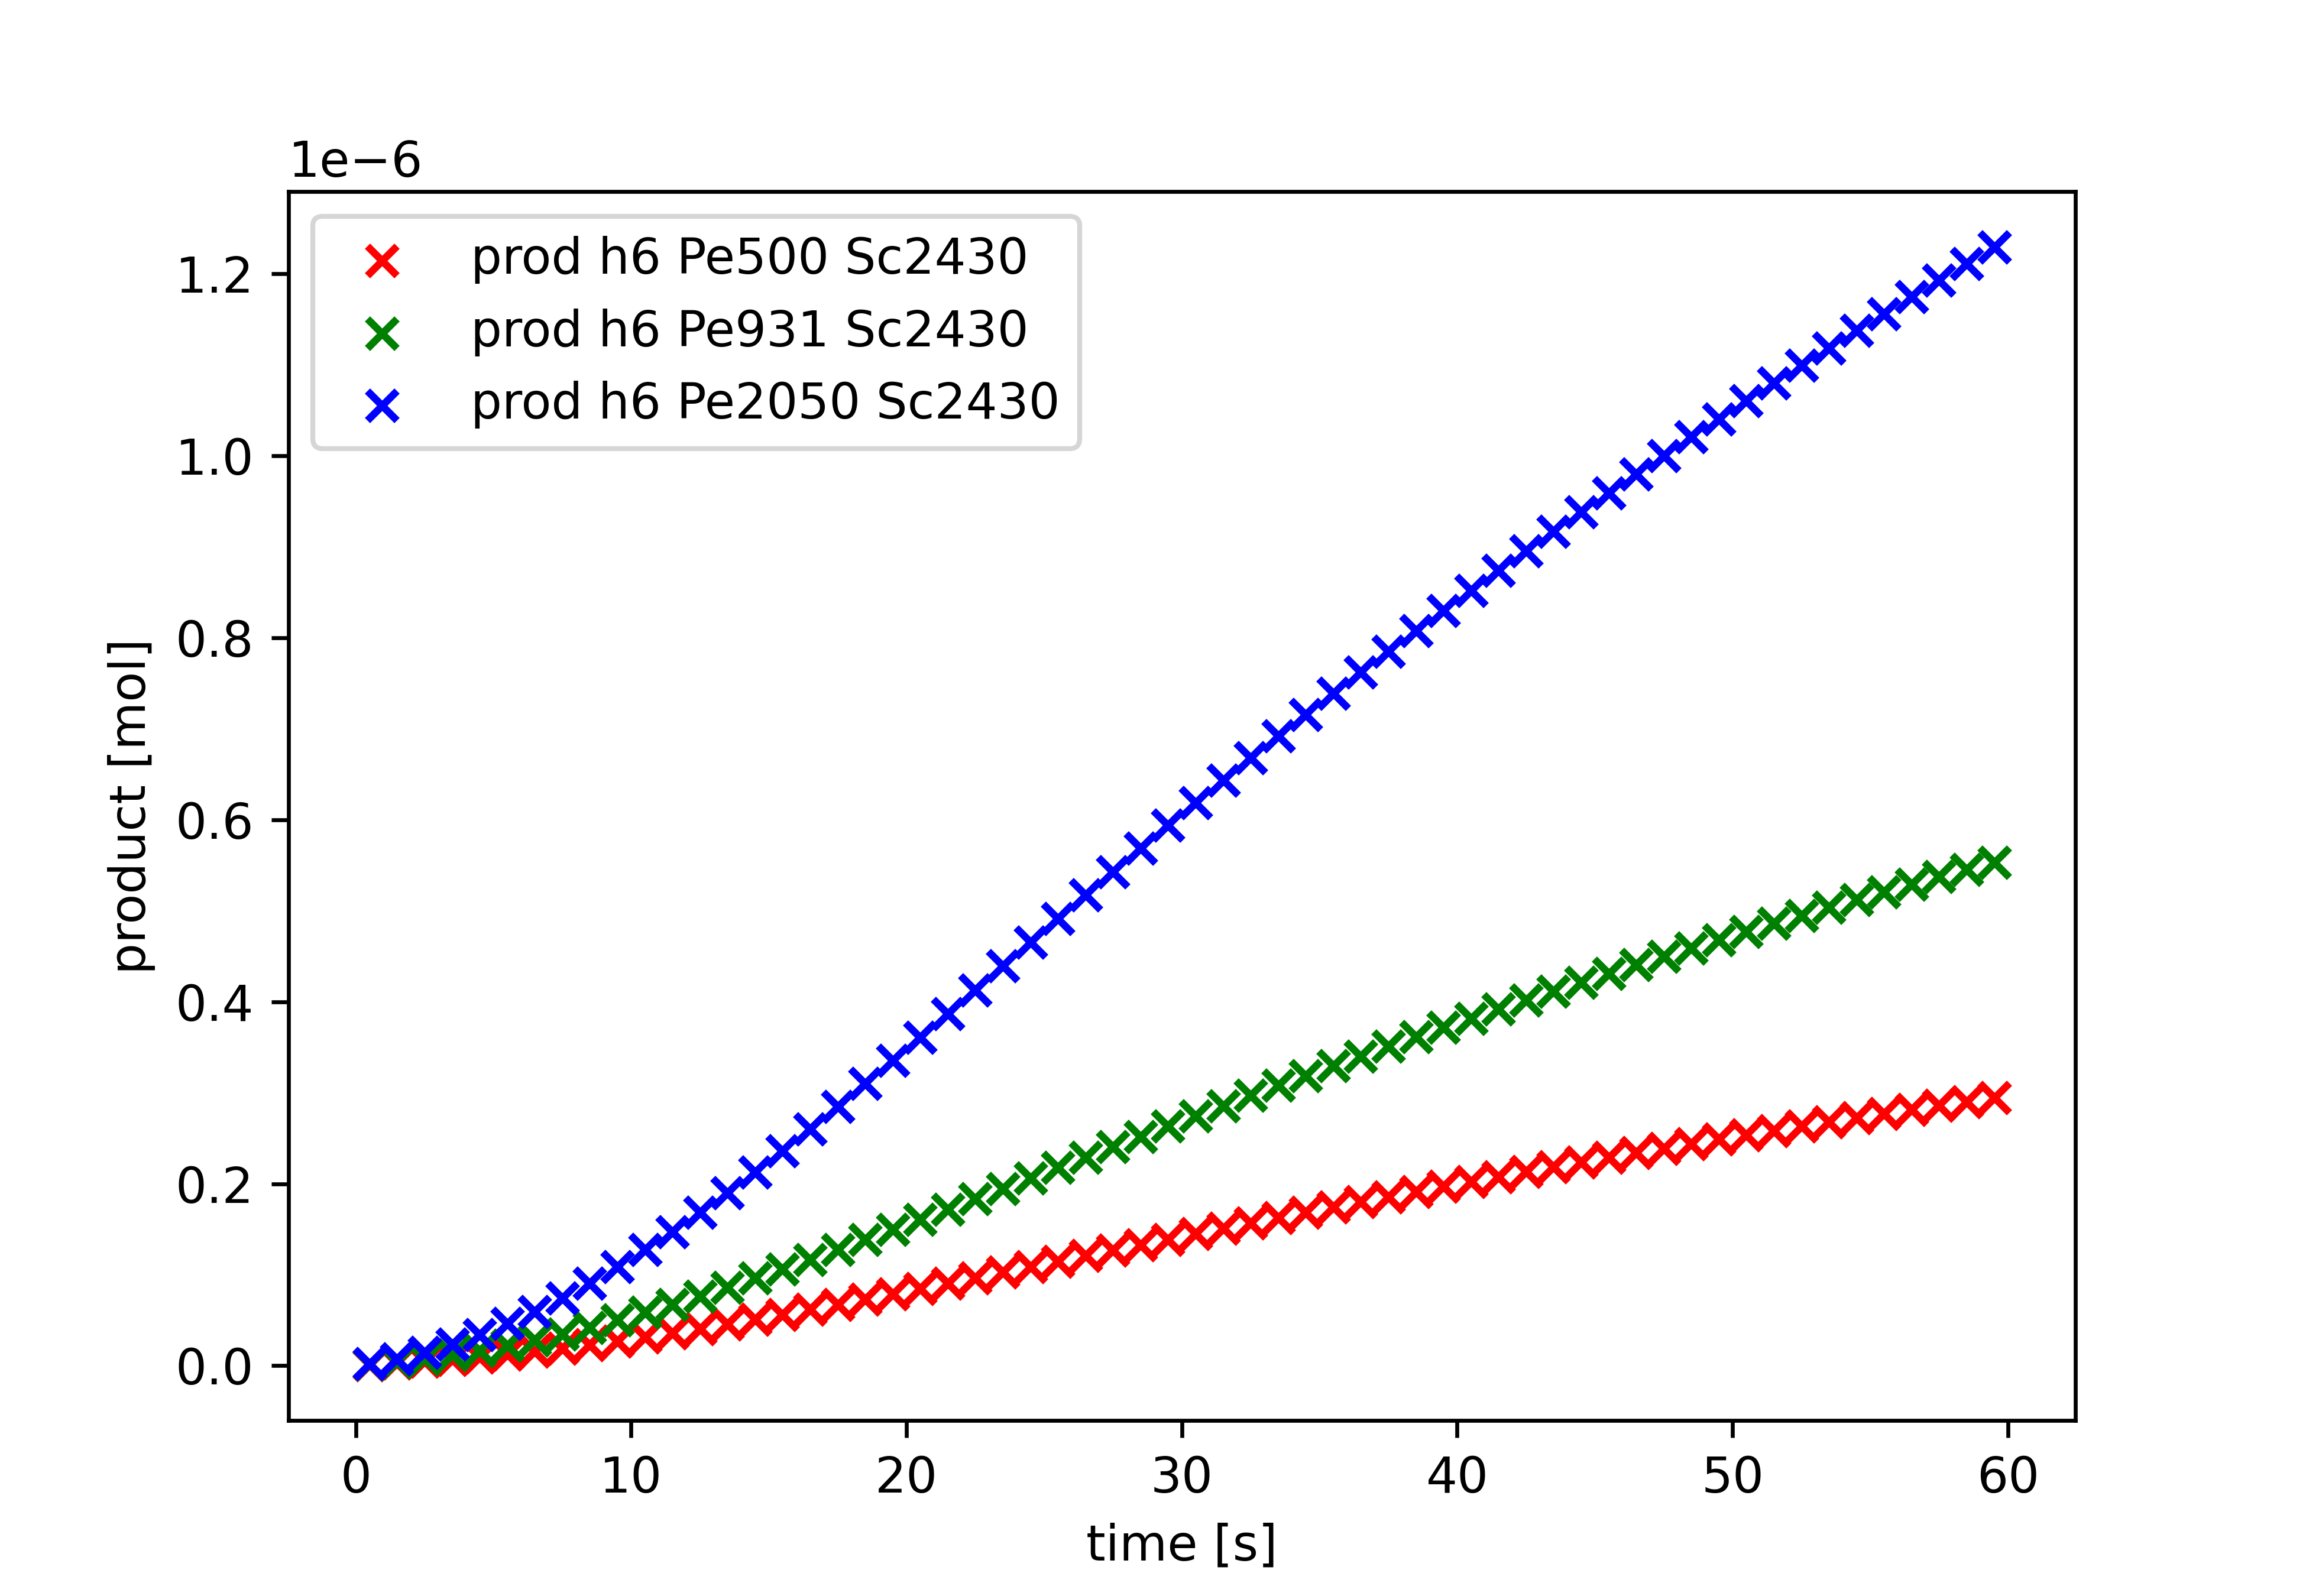
\includegraphics[width=.9\linewidth]{total_product_h6_Sc2430}
	\caption{total product for  h = 0.6mm Sc = 2430\label{fig: total_prod_h6_Sc2430}}
\end{figure}
\newline

The cases with a gap height of 0.6mm and a Schmidt number of 12000 are still in the phase of higher production rate throughout the hole simulation run. In \autoref{fig: h6_late_shapes} the front shapes are shown for a time of 60 seconds for both Schmidt numbers.
\begin{figure}[htb]
	\centering
	\subfloat[\centering Sc=2430]{{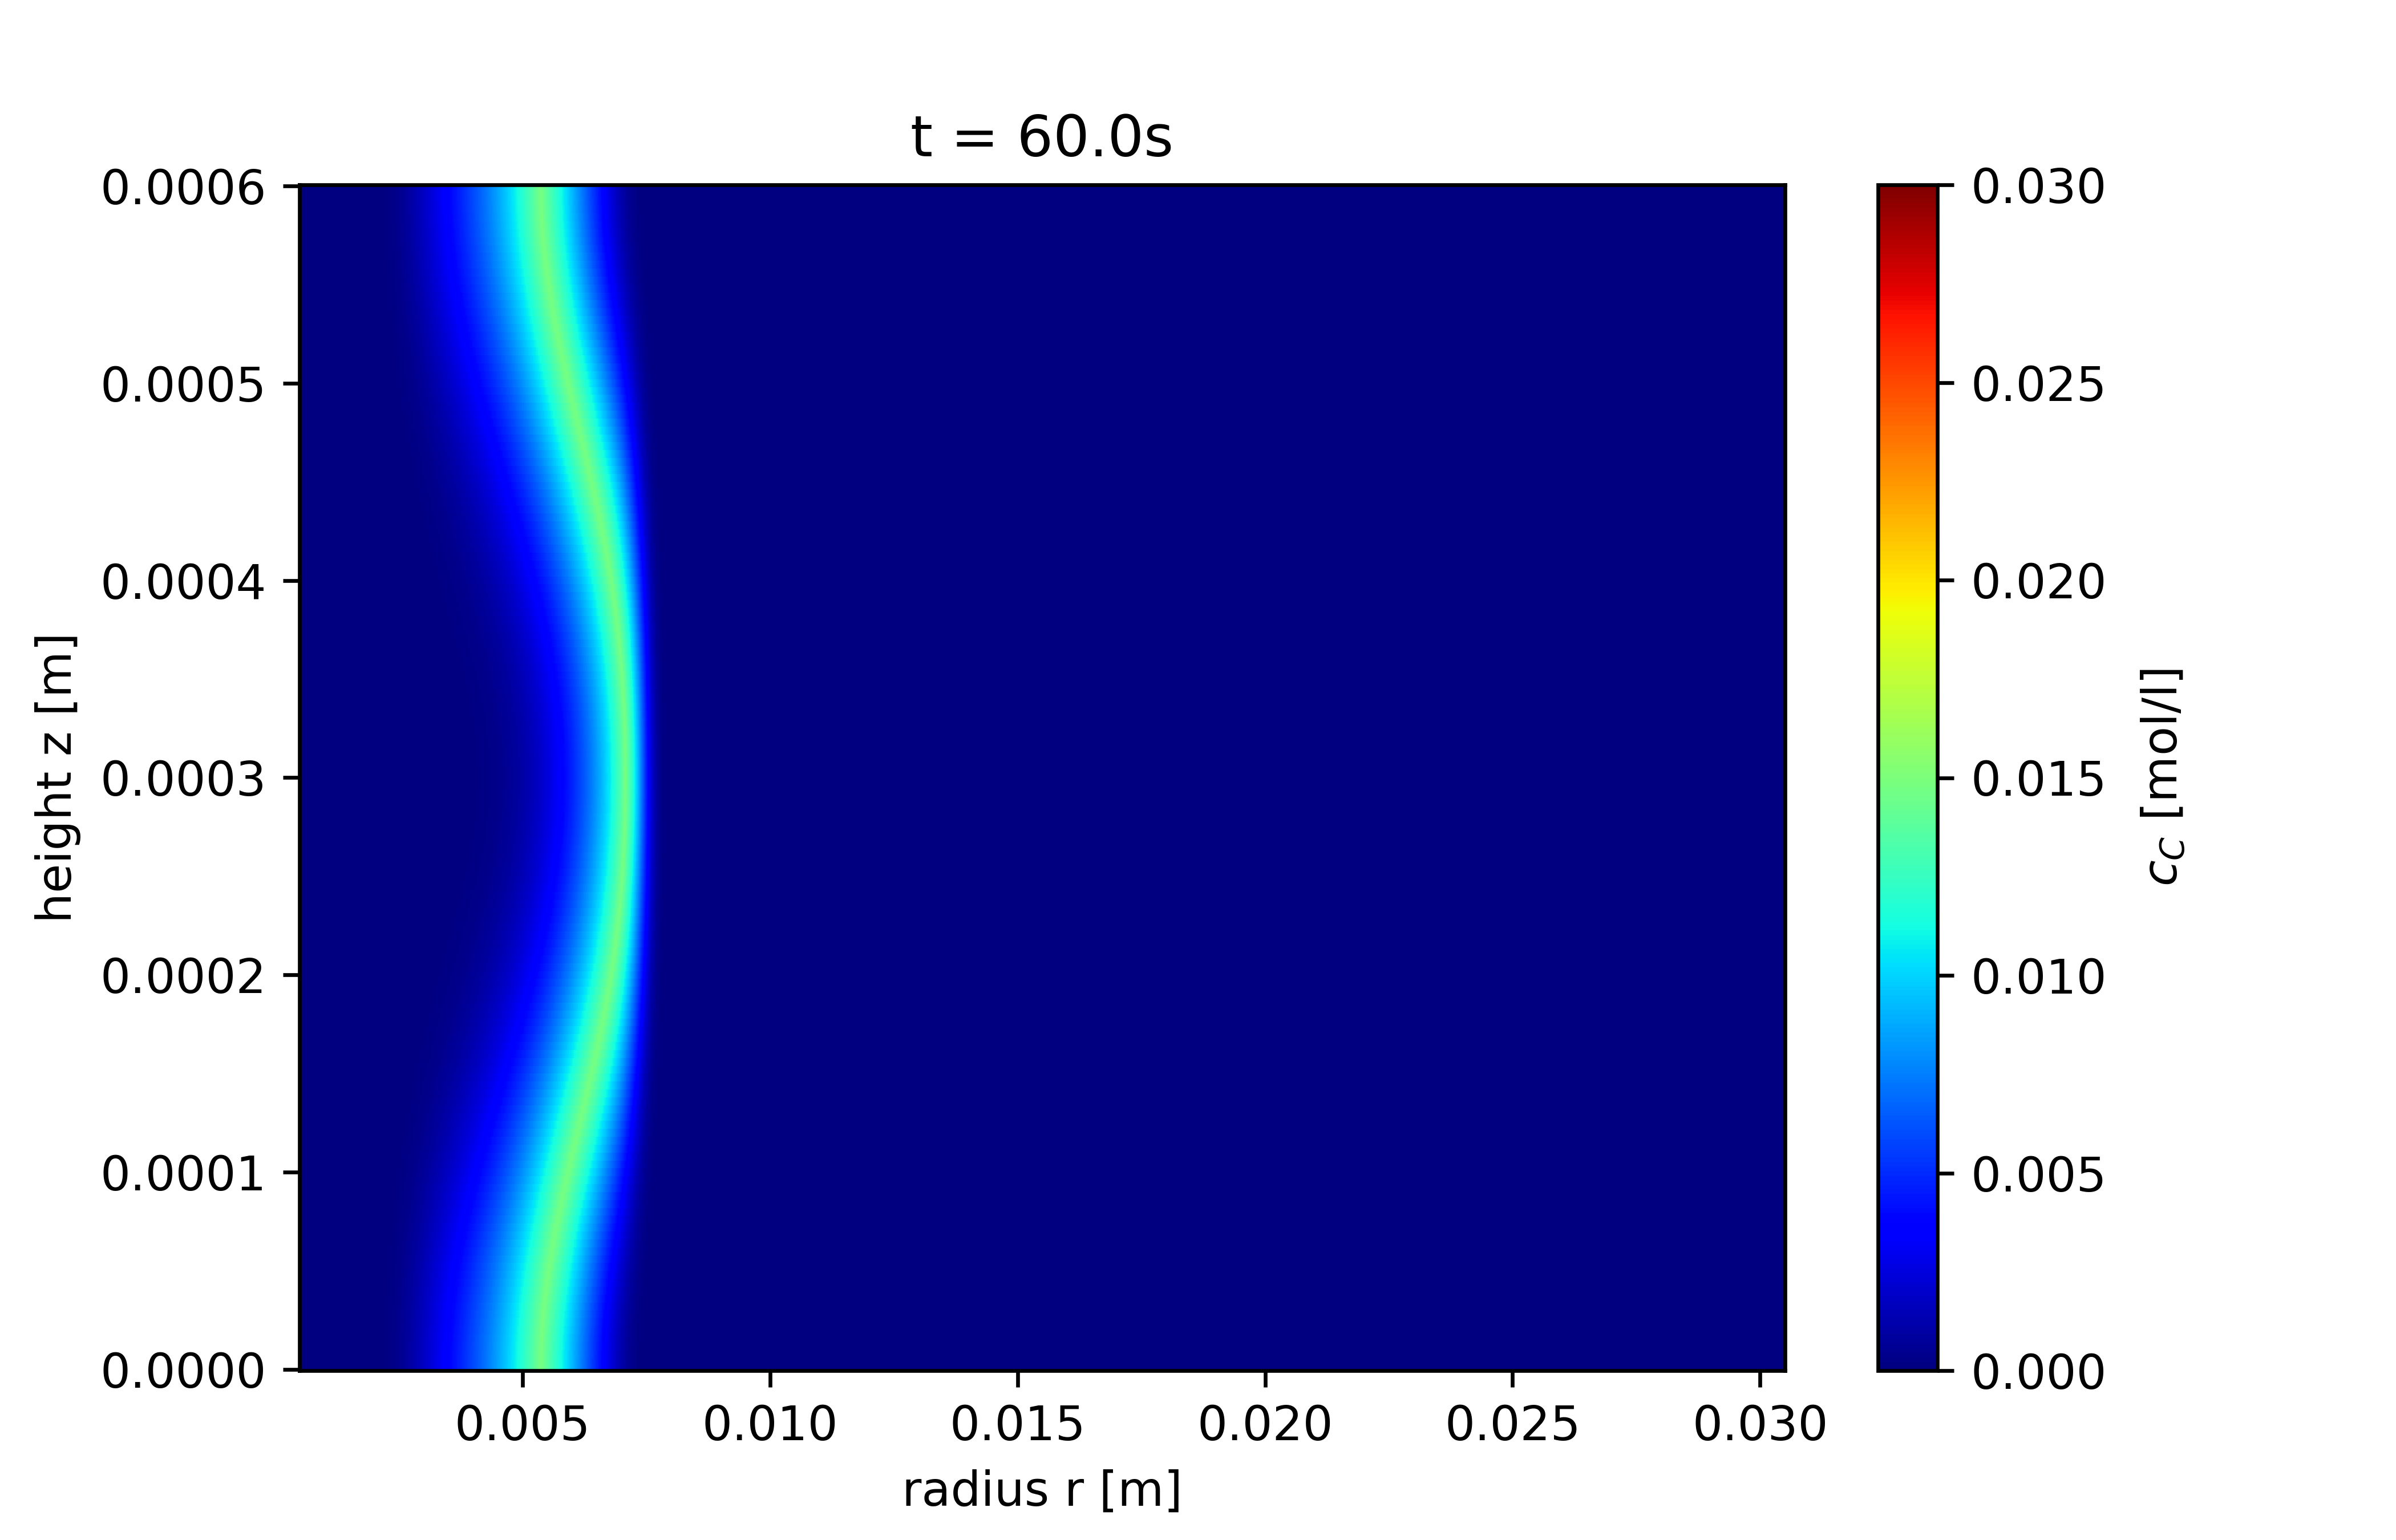
\includegraphics[angle=0, scale=0.41]{field_h6r3_P931E2_S243E3_concentration-fluid_c} }}%
	\qquad
	\subfloat[\centering Sc=12000]{{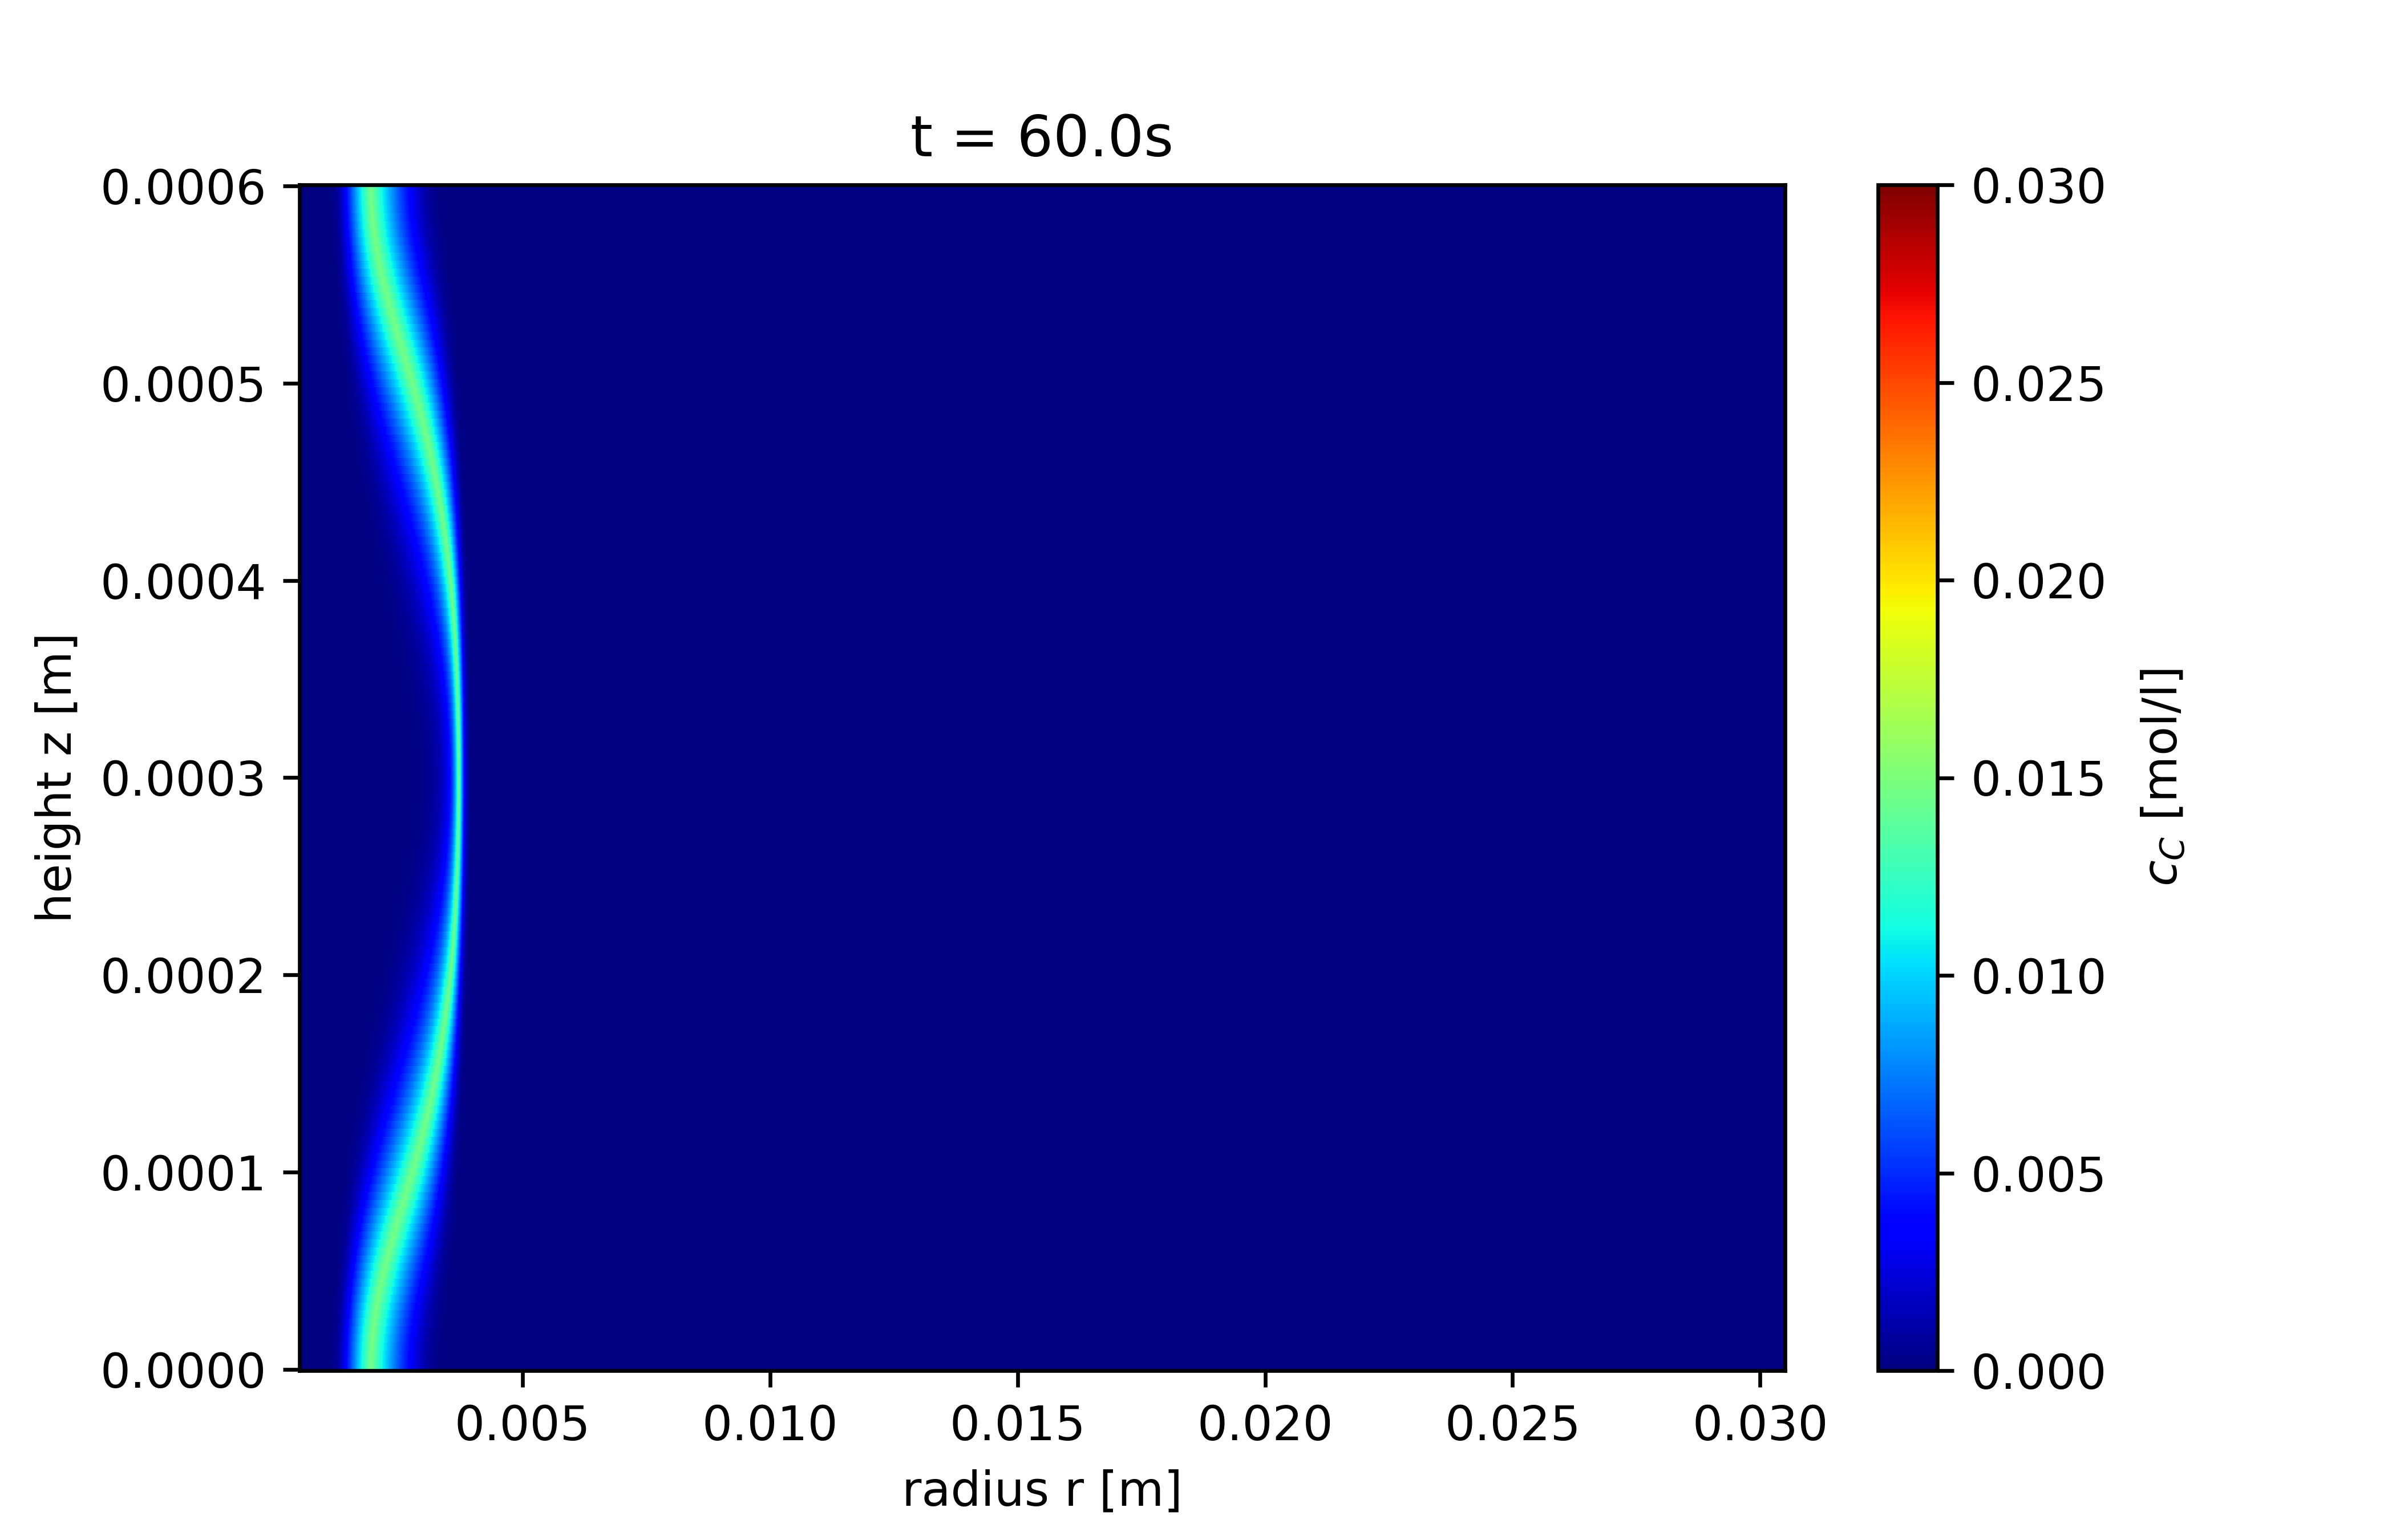
\includegraphics[angle=0, scale=0.41]{field_h6r3_P931E2_S120E4_concentration-fluid_c} }}%
	\caption{product concentration fields at t=60s for  h = 0.6mm  Pe = 931}%
	\label{fig: h6_late_shapes}%
\end{figure}
From the image showing the higher Schmidt number cases it can be seen that the front is still building over the hole gap height, so the reaction rate would remain high until that is accomplished. Comparing that to the lower Schmidt number case were the front has nearly reached its final form, only a slight decay is visible towards the end of the simulation. To get clearer evidence on when the production rate has reached its final constant value the simulations need to be run for longer times.

Within \cite{brau2020influence} a linear behaviour of the total amount of product created was found for a radial case. Therefore a linear fit is done on the data of the last 10 seconds for each case. In \autoref{tab: prod_rates} all rates are united.
\begin{table} [htbp]
	\centering
	\caption{production rates for all cases}
	\begin{tabular}{ cccc }
		\hline
		gap height [mm] & Pe & Sc & production rate [mol/s] \\
		\hline
		0.2 & 500 & 12000 & 5.815e-10 \\
		0.2 & 931 & 12000 & 1.064e-09 \\
		0.2 & 2050 & 12000 & 2.313e-09 \\
		0.2	& 500 & 2430 & 1.135e-09 \\
		0.2	& 931 & 2430 & 1.994e-09 \\
		0.2	& 2050 & 2430 & 4.136e-09 \\
		0.4 & 500 & 12000 & 1.215e-10 \\
		0.4 & 931 & 12000 & 2.255e-09 \\
		0.4 & 2050 & 12000 & 4.965e-09 \\
		0.4	& 500 & 2430 & 2.397e-09 \\
		0.4	& 931 & 2430 & 4.317e-09 \\
		0.4	& 2050 & 2430 & 9.242e-09 \\
		0.6 & 500 & 12000 & 1.196e-09 \\
		0.6 & 931 & 12000 & 2.246e-09 \\
		0.6 & 2050 & 12000 & 4.988e-09 \\
		0.6	& 500 & 2430 & 4.551e-09 \\
		0.6	& 931 & 2430 & 8.452e-09 \\
		0.6	& 2050 & 2430 & 1.874e-08 \\
		\hline
		\label{tab: prod_rates}
	\end{tabular}
\end{table}
It does not surprise that the highest values of the production rate can be seen within cases with the highest gap height and the higher Peclet numbers. Doubling the gap height from 0.2mm to 0.4mm seems to approximately double the production rate. That trend can be seen for both Schmidt numbers.
\newline

The production rate behaves similar on a principle level within all geometries investigated but the stages the fronts go through within the 60 second time span of the simulation are different for the different gap heights. 


\end{document}